\documentclass[letterpaper,twocolumn,10pt]{article}
\usepackage{usenix-2020-09}

% to be able to draw some self-contained figs
\usepackage{amsmath}
\usepackage[edges]{forest}
\usepackage{algorithm}
\usepackage{algorithmicx}
\usepackage{algpseudocode}
\usepackage{longtable}
\usepackage{colortbl}
\usepackage{tabularx}
\usepackage{tikz}
\usepackage{pgf-pie}
\usepackage{xcolor}
\usepackage{graphicx}
\usepackage{pifont}
\usepackage{array}
\usepackage{booktabs} % For prettier tables
\usepackage{multirow} % For multirow cells
\definecolor{codeblue}{RGB}{0,0,245}
\definecolor{codegreen}{RGB}{0,200,0}
\definecolor{codered}{RGB}{139,0,0}
\definecolor{codegray}{RGB}{128,128,128}
\definecolor{codepurple}{RGB}{128,0,128}
\definecolor{codeorange}{RGB}{255,165,0}
\definecolor{codeblack}{RGB}{0,0,0}
\definecolor{gray!25}{RGB}{200,200,200}
\definecolor{Lavender}{RGB}{235,220,245}
\definecolor{PastelGreen}{RGB}{220,245,220}
\definecolor{LightPeach}{RGB}{245,230,220}
\definecolor{highlighteryellow}{RGB}{255, 255, 153}
\definecolor{SoftYellow}{RGB}{245,245,220}
\definecolor{SoftLavender}{RGB}{230,220,245}
\definecolor{SoftRose}{RGB}{245,220,233}
\definecolor{SoftMint}{RGB}{220,245,233}
\definecolor{SoftOrange}{RGB}{245,230,220}
\definecolor{darkgreen}{rgb}{0.0, 0.5, 0.0}
\definecolor{lightgray}{gray}{0.9}
\newcolumntype{"}{@{\hskip\tabcolsep\vrule width 1pt\hskip\tabcolsep}}
\newcommand{\halfdot}{
    
\begin{tikzpicture}
        \fill[black] (0,0) arc (90:270:0.12cm) -- cycle;
        \fill[white] (0,0) arc (-90:90:0.12cm) -- cycle;
    \end{tikzpicture}
}
\newcommand*\circled[1]{\tikz[baseline=(char.base)]{
            \node[shape=circle,fill=black,text=white,inner sep=0.8pt] (char) {#1};}}


\definecolor{SoftRed}{RGB}{255,200,200}
\definecolor{SoftGreen}{RGB}{200,255,200}
\definecolor{SoftPurple}{RGB}{220,200,255}
\definecolor{SoftBlue}{RGB}{200,220,255}
\usepackage{multirow}
\usepackage{amsmath}
\usepackage{times,url,color,soul,xspace,enumitem}
\usepackage{graphicx}
\usepackage{caption}
\usepackage{tabularx}
\usepackage{subcaption}
\usepackage{comment}
\usepackage{xspace}
% to be able to draw some self-contained figs
\usepackage{tikz}
\usepackage{amsmath}
\usepackage[inline,draft,nomargin,index]{fixme}

\usepackage[utf8]{inputenc}
\usepackage{amsmath, amsthm, amssymb}
\newtheorem{definition}{Definition}
% \microtypecontext{spacing=nonfrench}


% \usepackage{cleveref}
% \crefformat{section}{\S#2#1#3} % see manual of cleveref, section 8.2.1
% \crefformat{subsection}{\S#2#1#3}
% \crefformat{subsubsection}{\S#2#1#3}

\newcommand{\linyun}[1]{\textcolor{red}{#1}}
\newcommand{\yd}[1]{\textcolor{blue}{#1}}

 %\newcommand{\camready}[1]{\hl{#1}}
% \newcommand{\camready}[1]{#1}
 %\usepackage{ulem}
 %\newcommand{\camdel}[1]{\sout{#1}}

%\newcommand{\camready}[1]{#1}
%\newcommand{\camdel}[1]{#1}

\newcommand{\dc}{datacenter\xspace}
\newcommand{\tool}{{Refuter}\xspace}

%-------------------------------------------------------------------------------
\begin{document}
%-------------------------------------------------------------------------------

%don't want date printed
\date{}

% make title bold and 14 pt font (Latex default is non-bold, 16 pt)
\title{\Large \bf \tool: A Trojan-oriented Explainable Intrusion Detection Approach via Verifiable Knowledge from Large Language Model}

% %for single author (just remove % characters)
% \author{
% {\rm Me}\\
% VU, Amsterdam
% \and
% {\rm Other Smart People}\\
% VU, Amsterdam
% % copy the following lines to add more authors
% % \and
% % {\rm Name}\\
% %Name Institution
% } % end author

\maketitle
% \tableofcontents

%-------------------------------------------------------------------------------
\begin{abstract}
%-------------------------------------------------------------------------------
Advanced Persistent Threat (APT) attacks have become a pressing concern within critical sectors, including banking, military, and government, owing to their stealthy nature and prolonged presence. Traditional detection methods, such as those reliant on provenance graphs, struggle to capture subtle attack signals, primarily due to the limited information and knowledge encapsulated within log files.
Furthermore, these approaches often yield ambiguous and non-explainable results and cannot cope with the continual evolution of attack strategies. 
To address the compelling imperative for security personnel to swiftly and comprehensively detect and understand the attacks, the development of more transparent and advanced detection techniques becomes of paramount importance. 
% YD: I comment out the following sentences.
% The solution lies in technologies capable of rapidly enhancing these methods with added knowledge.
% Fortunately, with recent advancements, Large Language Models (LLMs) have emerged as particularly promising in knowledge-centric tasks. 
In this work, we propose \tool, an effective and explainable APT attack-detection method that merges the effectiveness of provenance graph-based APT detection with the knowledge acquisition capabilities of Large Language Models (LLMs).
Specifically, \tool first utilizes LLMs to extract knowledge of system processes and construct a more detailed profile for each process. Then, \tool transforms each profile into a set of key constraints, upon which \tool can perform comprehensive threat detection.
Drawing on the extensive knowledge gained through LLMs, \tool can effectively reduce ?\% false alarms and uncover ?\% more attack patterns that typically evade existing methods. This heightened capability also enables  \tool to provide deeper insights into the potential threats detected. Additionally, benefiting from its automated extraction capability, 
%which facilitates swift profile updates and eliminates the dependence on the predefined attack patterns, 
\tool has the ability to effectively and efficiently identify novel and evolving threats.
% enables swift profile updates, and without relying on predefined attack patterns, \tool can identify novel and evolving threats.
% As we spent around 21 minutes and 3.5\$ on each of 100 system profiles, \tool effectively reduces false alarms and provides deeper insight into threats, facilitating faster and more informed responses.

\end{abstract}

%-------------------------------------------------------------------------------
\section{Introduction}
%-------------------------------------------------------------------------------
Advanced Persistent Threats (APTs) have long known as a formidable adversary in the cyber landscape,
regarding their stealthy and persistent nature, 
as well as exceptionally damaging consequence \cite{xx, xx, xx, xx, xx}.
After achieving unauthorized access, 
the attackers can deploy their malware on the server to 
gather information and credentials of the victim \cite{xx, xx},
spread their influence across the local network \cite{xx, xx}, and
maintain remote access to control the compromised servers \cite{xx, xx}.

As one of the most important toolkits in attackers' arsenal,
trojans, a type of malware often disguising as a legitimate software,  
are often used in APT attacks.
The malware allows the attackers to 
be evasive from user screening and
exploit the compromised system for a longer time.
For example in \linyun{DARPA DC} dataset, 
a trojan can disguise itself as a system process \textit{svchost.exe} (see Section~\ref{sec:motivation} for more details)
to increase its plausibility and avoid the detection,
which lasts for \linyun{XX} years.
Further, the MITRE ATT\&CK Framework reports \linyun{???\%} of the trojan-relevant attacks.
A growing number of evidence shows that trojan-based APT attack is 
pervasive \cite{valeros2020growth, xx}. 


As countermeasures, industrial and academic solutions \cite{karantzas2021empirical, cheng2023kairos,alsaheel2021atlas,han2020unicorn,inam2022sok,han2021sigl} are emerging to
report the post-intrusion behaviors based on the collected system logs,
which can generally fall into rule-based approaches \cite{milajerdi2019holmes,milajerdi2019poirot,hossain2020combating} and learning-based approaches \cite{liu2018towards,hassan2019nodoze,hassan2020we, wang2022threatrace,han2020unicorn,wang2020you}. 

\noindent\textbf{Rule-based Approaches.}
The rule-based solutions are usually commercial products \cite{milajerdi2019holmes,milajerdi2019poirot,hossain2020combating} such as SIEM (Security Information and Event Management) and \linyun{YYY} detect APT attacks via predefined security rules.
While the rules can be useful in a way,
they can be either too strict so that they miss reporting true positives or
too general so that a large number of false alarms exhaustively costly to validate,
undermining users' confidence in the tools.

\noindent\textbf{Learning-based Approaches.}
Many researchers consider the problem of intrusion detection as a supervised-learning problem \cite{liu2018towards,hassan2019nodoze,hassan2020we} or an unsupervised-learning problem \cite{wang2022threatrace,han2020unicorn,wang2020you}.
Therefore, different representations \cite{zeng2021watson, zengy2022shadewatcher} (including graph embedding, context-aware information flow, etc.) are extracted and learned from the system logs.
If the logs or its representation (nodes on the log-derived provenance graph) can be attached with labels (malicious or not),
we can learn a classification model to predict the attacks \cite{xxx}.
Otherwise, we define and learn the normality on the log representation (e.g., graph \cite{manzoor2016fast,han2020unicorn,li2021hierarchical,yang2023prographer,cheng2023kairos}, path \cite{wang2020you,alsaheel2021atlas}, text sequence, etc.), and detect the attacks (or the anomaly) by
defining a distance in the representation space.

While the learning-based approaches can leverage 
the AI-powered infrastructure (e.g., Graph Neural Network \cite{xx}, BERT \cite{xx}, etc.) from the machine learning community,
they still suffer from the following insufficiencies.

\begin{itemize}[leftmargin=*]
  \item \textbf{Explainability:}
    While the attack can be predicted in a supervised-learning or unsupervised-learning solution,
    the numeric representation is not straightforward for a security engineer to 
    validate the potential false alarm.
    Therefore, the security engineers still need to pay non-trivial efforts to 
    track the event causality from the system logs.
    Any false alarm can undermine users' trust in the solution.
  \item \textbf{The Quality of Training Dataset:}
    It is non-trivial to label high-quality training dataset in such a security application.
    More often than not, the attack logs are the minority, which introduces inherent data imbalance problem.
    As a result, it is non-trivial to fill the gap between the experimental and the practical performance.
    %Thus, it is unclear whether the performance of the trained model can be well generalized in practice.
  \item \textbf{Evolving Attacks:}
    Finally, the learned models can be dependent on the training dataset of attack logs.
    In the cat-and-rat game of APT security,
    novel attacks can always emerge, 
    leaving both the training dataset and its derived model obsolete.
\end{itemize}


In this work, we propose \tool,
a trojan-oriented explainable intrusion detection technique,
to report disguising trojans in APT attack without training on \textit{any} attack datasets.
Our insight lies in that,
while the general explainable intrusion detection technique can be challenging,
trojan-induced APT attacks exhibit a natural explanation based on
the inconsistency between 
(1) trojan's claimed legitimate program (e.g., \textit{svchost.exe}) and
(2) trojan's actual behavior or true intention (e.g., \textit{delete a registry file}).
In this regard, 
\tool considers the trojan-induced intrusion detection problem as a problem of
detecting a ``lie'' in the runtime system.
\tool is designed as a counter-factual solution to find such inconsistency,
which consists of two steps, i.e., 
(1) behavioral reference construction and
(2) runtime behavioral validation.

\noindent\textbf{Behavioral Reference Construction.}
Given a claimed system process, \tool constructs the behavioral reference in the form of 
verifiable logical proposition describing either
(1) the fact which the process has to meet (e.g., the process with name \textit{svchost.exe} must be launched by \textit{\linyun{process-name.exe}} at the location \textit{C://system//service.exe}), or
(2) the temporal relation between two events 
(e.g., the event that \textit{svchost.exe} reads \linyun{\textit{read XX.dll}} must happen before the event \textit{svchost.exe} writes \linyun{\textit{read XX.dll}}).
\tool extracts composition proposition regarding both disjunction and conjunction
to represent the behaviorial invariants of a system process.

\noindent\textbf{Runtime Behavioral Validation.}
During the system runtime,
given a claimed process (e.g., \textit{svchost.exe}),
\tool transforms its runtime system logs into runtime logical propositions, 
representing a sequence of runtime events.
By concatenating the reference logical propositions and runtime logical propositions,
we can verify whether the runtime behaviors of a claimed process violate its behaviorial invariance.
If yes, the violation (i.e., inconsistency) is raised as both the alarm and its explanation.


To construct the behaviorial reference, 
we design a cross-validation technique to extract verifiable knowledge from LLM (Large Language Model) such as ChatGPT.
On one hand, 
we adopt in-context learning solution to guide LLM to 
introduce the runtime knowledge of a system process in a \textit{verifiable} way.
On the other hand,
we validate the knowledge by running the process in a sandbox.
For the verified knowledge,
we extract the fact and the temporal relation among the events
as logical propositions.


We evaluate \tool with extensive experiments by building a Caldera-based benchmark,
simulating 10 trojan-induced APT attack scenarios including 
4 prevalent stealth techniques \cite{xx}, 
23 malicious functionalities \cite{xx}, and 
4 prevalent stealth techniques \cite{xx}.
In the experiment, \tool generates the behaviorial profile of \linyun{100} system processes
at the cost of \$3.5 per profile.
Our experiments show that 
\tool is effective in reporting trojan-based APT attack comparing to the state-of-the-art solutions (with the precision of \linyun{100\%} and the recall of \linyun{??\%}),
at the cost of minimum runtime overhead (of on average \linyun{3s}).
Further, our wild study shows that \tool can detect \linyun{??} trojan-based attacks on \linyun{??} systems.

In summary, we make the following contributions:
\begin{itemize}
  \item We propose an explainable intrusion detection technique \tool to report both the alarm and its explanation in a unified way. 
      To the best of our knowledge, we are the first to detect intrusion against constructed behaviorial profile of system process.
  \item We deliver \tool which can 
    (1) construct the behaviorial invariant of a given process by enforcing LLM to output trustworthy and verifiable propositions and
    (2) validate an arbitrary system process against the constructed profile.
  \item We deliver our Caldera-based benchmark, which simulates 10 trojan-induced attacks. 
    The benchmark is extensible for introducing more attacks.
  \item We conduct extensive experiment to evaluate \tool, showing its performance regarding high precision in both the detection results and the generated explanation.
\end{itemize}
 



%Further, we collected malware used in known APT attacks from public repositories and websites, revealing that camouflage techniques are ubiquitous in such attacks.
%As a result, the detection rates and range of threats identified by ProCon were consistently superior to those of existing solutions. With our realistic and multifaceted attack simulations, ProCon's robust performance accentuates its transformative potential in cybersecurity, offering organizations a stronger defense against APT threats.


%\textbf{Statistical-based} techniques \cite{liu2018towards,hassan2019nodoze,hassan2020we}, although intuitive, grapple with false positives, making it tough to differentiate genuinely anomalous behaviors from benign novelties.
%In sum, while each technique offers nuanced advantages, a comprehensive method that addresses all four dimensions and seamlessly tackles every facet of APT detection remains an open challenge.

%coupled with the extensive damage they can inflict, make them exceptionally challenging to detect and mitigate.
%In light of this, we embarked on an exhaustive study of current commercial Endpoint Detection and Response (EDR) products \cite{karantzas2021empirical} and provenance graph-based solutions \cite{cheng2023kairos,alsaheel2021atlas,han2020unicorn,inam2022sok,han2021sigl}. Our deep dive into these systems allowed us to identify critical gaps and challenges. Specifically, we distilled the problems facing current solutions into four key dimensions:

%While data provenance-based threat detection has emerged as a promising approach against the covert Advanced Persistent Threats (APTs), current methodologies exhibit specific shortcomings, failing to satisfy all four dimensions concurrently.
%% \yd{YD: Maybe can merge the following content into above four key dimensions?}
%
%On the other hand, while \textbf{anomaly-based} techniques \cite{wang2022threatrace,han2020unicorn,wang2020you} are adept at spotting deviations, their outcomes often lack transparency and pose challenges for integration into commercial products. Within this realm, graph \cite{manzoor2016fast,han2020unicorn,li2021hierarchical,yang2023prographer,cheng2023kairos} and path-based methods \cite{wang2020you,alsaheel2021atlas} tend to detect only those attacks that leave discernible traces on the graph or path, yielding results that are too macroscopic. Node-based methods provide finer granularity but can sometimes oversimplify intricate attack behaviors.
%Knowledge graph embedding techniques\cite{zeng2021watson,zengy2022shadewatcher} may have difficulty representing a single process accurately with a single vector due to the diversity of node functions and similarities between normal nodes and malicious nodes.





%\begin{itemize}[leftmargin=*]
%    \item \textbf{Insufficient information within Log Data}: Effective intrusion detection hinges on the richness and comprehensiveness of audit logs. Recent research \cite{gandhi2023rethinking} underscores a concerning deficiency: current logging systems capture insufficient information for reliable attack detection. Solely relying on these raw logs may result in a low attack detection coverage. To further enhance this capability, we aim to detect more attacks without increasing the granularity of log collection. A need exists to integrate more detailed knowledge into our system, especially in understanding the precise meanings of entities within logs, including process names, registry files and dynamic link libraries (DLLs), etc. By enriching our logs with more information and knowledge, we stand a better chance of detecting a wider range of attacks, especially the stealthy behaviors often employed in APT attacks.
%    \item \textbf{Attack Agnosticity}:
%    Zero-day vulnerabilities (malware or flaws not yet identified by security analysts), especially in APT attacks, require detection systems that are not bound by pre-existing signatures or indicators. Anomaly detection \cite{wang2020you, alsaheel2021atlas, han2020unicorn}, stands out as the most effective technique for identifying such zero-day exploits. Therefore, an optimal method of detecting these unknown threats would not rely on known attack patterns.
%    \item \textbf{Evolving Threats}: Advanced Persistent Threats (APT) represent dynamic, sustained, and sophisticated threats. Professional attacker groups continuously innovate, targeting an ever-expanding array of system processes and adapting to the latest defensive measures. This evolving landscape necessitates detection methods that can swiftly identify and adapt to emerging attack paradigms.
%    \item \textbf{Transparency}: The value of detection alerts lies in their clarity. For security personnel, a clear understanding of the 'why' and 'how' behind detection can drive quicker and more effective interventions. By providing clear explanations, system administrators will have a better understanding of the threat landscape, allowing them to respond to threats faster and in a more knowledgeable manner.
%\end{itemize}




%The primary impediments to addressing the current challenges in APT detection can be attributed to the inherently knowledge-intensive nature of the cybersecurity domain. When faced with audit logs that present insufficient information, there's an acute need to augment them with supplementary domain-specific knowledge. This supplemental knowledge becomes even more crucial when attacks evolve or present themselves in stealthy manners. Moreover, a well-rounded domain understanding also serves as a basis for explaining detection results, enhancing transparency for security analysts. Thus, the key to overcoming these challenges lies in the ability to swiftly and effectively harness extensive cybersecurity knowledge.
%Fortunately, Large Language Models (LLMs) have demonstrated remarkable prowess in recent years. These models are capable of understanding human-like text intricacies and have demonstrated efficacy across a wide range of domains, especially those requiring rapid knowledge extraction. There is an important question here: \textit{Can LLMs be effectively leveraged in cybersecurity to improve detection methods for stealthy and evolving APT attacks?}

%In response to this crucial question, we focus on addressing these dimensions, combining knowledge extraction prowess of LLMs with the structural expertise of provenance graphs, aiming to detect APT. To accomplish our goal, we want the LLMs to automatically identify key constraints associated with system processes. These constraints are then transformed into actionable rules that serve as vital tools for detecting attacks. It is possible to detect attacks without increasing the granularity of our log data by thoroughly extracting and understanding log entities, such as program names, dynamic link libraries (DLLs), and registers. In addition, LLMs' vast knowledge repository allows us to discover unknown and evolving threats in addition to interpreting the nature of the attacks. As a result, we cover the four dimensions previously discussed.

%As we all known, the use of LLMs for contract process profiling has both advantages and challenges. It is evident that LLMs have extensive knowledge of process behavior and are able to explain their outputs. However, following detailed practice, we found that LLMs construction processes presented challenges due to  \textit{difficulty handling complex scenarios},
%\textit{context reliance}, \textit{memory limitations}, and \textit{the possibility of generating inaccurate information or hallucinations}.

%To address these challenges, we introduced ProfileGuard, a method for automated system process profile construction using LLMs.This method involves:

%\begin{itemize}
%    \item Process Behavior Tree Construction: We attempted to capture as many behaviors as possible for each process, creating a behavior tree. Using a "self-ask" approach, the LLMs continuously expanded its knowledge of this tree. This tree also played a pivotal role in providing the LLMs with contextual depth.
%    \item Command Execution: Based on the behavior tree, the LLMs scripted and executed commands for relevant behaviors.
%    \item Constraint Extraction: We designed a hybrid method that combines traditional programming techniques With queries to the LLMs to extract different process constraints.
%    \item Validation: A two-tiered validation approach has been implemented to validate the model's outputs. In the first tier, we execute actual commands and verify them against real-world logs, followed by a multi-round debate among the LLMs to validate their responses and reasoning.
%\end{itemize}
%We will delve into the mechanics of our design in detail in Section~\ref{sec:motivation}.






\section{Related work}

% \paragraph{Stealthy APT Attacks}
% Advanced Persistent Threats (APTs) are sophisticated, targeted, evolving, and steathy cyberattacks launched by specialized groups against high-risk entities, such as nuclear power plants, banks, and governments. APTs are using stealthy tactics such as name obfuscation\cite{cybereason2023,checkpoint2021,intrinsec}, process injection\cite{checkpoint2020,fsecure2019}, process hollow\cite{secureworks}, side-loading DLLs\cite{mitre_g0022,mitre_g0016}, and manipulating legitimate system utilities in order to bypass traditional security defenses due to the dynamic cyber threat landscape\cite{barr2021survivalism}. An example is Process injection, a popular technique for enabling malicious code to run within another process's address space.  Additionally, attackers use tools like \textit{rundll32.exe} to execute benign binaries and \textit{powershell.exe} to launch script-driven attacks\cite{li2019effective}. By exploiting these widely recognized and trusted tools, adversaries can discreetly penetrate and control their target systems.

\paragraph{Provenance Graph-Based APT Detection}
% Chenyan  usenix chair
% Threat Detection and Investigation with System-level Provenance Graphs: A Survey
% CONAN: A Practical Real-time APT Detection System with High Accuracy and Efficiency
% Effective and Light-Weight Deobfuscation and Semantic-Aware Attack Detection for PowerShell Scripts
% AttacKG: Constructing Technique Knowledge Graph from Cyber Threat Intelligence Reports
% RATScope: Recording and Reconstructing Missing RAT Attacks for Forensic Analysis with Semantics on Windows
% CONAN: A Practical Real-time APT Detection System with High Accuracy and Efficiency

% PC member
% Kangkook Jee
% You Are What You Do: Hunting Stealthy Malware via Data Provenance Analysis

% Ivan Martinovic
% Survivalism: Systematic Analysis of Windows Malware Living-Off-The-Land

% Z. Berkay Celik
% ATLAS: A Sequence-based Learning Approach for Attack Investigation

% Xiapu Luo
% D IST D ET: A Cost-Effective Distributed Cyber Threat Detection System

% Adil Ahmad
% Rethinking System Audit Architectures for High Event Coverage and Synchronous Log Availability




Provenance graph-based methods are becoming increasingly popular in detecting stealthy APT attacks, due to their ability to identify a variety of host-based threats. There are three main detection methods based on Provenance graphs: anomaly-based detection, misuse-based detection, and statistics-based detection.

\paragraph{Learning-based Approaches}
Anomaly-based detection techniques train models on benign behaviors, identifying deviations as potential cyber-attacks. Although these methods can detect threats with impressive accuracy by integrating audit record semantics into threat analysis, existing learning solutions often fail to provide insightful and explicable results, which can sometimes compromise their practical utility.

\noindent
{\bf Graph-based Methods.} Graph-based anomaly detection requires extensive training datasets and is computationally intensive. The researchers have embedded provenance graphs into vector space and developed tools such as StreamSpot \cite{manzoor2016fast} and Unicorn \cite{han2020unicorn} to analyze information flow graphs. Despite Unicorn's superior performance due to its thorough graph analysis, both methods face challenges in detecting stealthy threats due to graph kernel limitations. In the same way, IPG \cite{li2021hierarchical} and ProGrapher \cite{yang2023prographer} use graph-level approaches, but struggle with similar issues as StreamSpot and Unicorn. Despite the fact that many systems attempt to use data provenance for threat detection, methods that combine scope and timeliness are needed. The remarkable capabilities of KAIROS \cite{cheng2023kairos} make it an excellent competitor.

\noindent
{\bf Path-based Methods.} By extracting causal paths from the provenance graph, these models leverage existing learning methodologies. ProvDetector \cite{wang2020you} analyzes the provenance graph for malware detection by converting paths into embedded forms and utilizing the Local Outlier Factor method. However, due to the diversity of host-based threats, relying solely on paths from the provenance graph is not sufficient. ATLAS \cite{alsaheel2021atlas}uses sequence models to distinguish attack patterns, recognizing that explicit and abstract strategies may be analogous, regardless of vulnerabilities exploited and payloads executed.

\noindent
{\bf Node-based Methods.} To detect stealthy abnormal behavior without knowing prior attack patterns, ThreaTrace\cite{wang2022threatrace} employs a GraphSAGE-based framework that learns every benign node's role in a system data provenance graph. To address data imbalance and improve detection, ThreaTrace provides a multi-model framework to learn different types of benign nodes.

\noindent
{\bf Knowledge Graph Embedding-based Methods.} Tools like Shadewatcher\cite{zengy2022shadewatcher} and Watson\cite{zeng2021watson} both use knowledge graph embedding to represent the semantics of individual nodes and edges. This is a promising approach. The tactics used by attackers can, however, be varied and complex. An attacker who creates a malicious node that closely mimics a genuine node makes it difficult to identify it. Process hollowing attacks, for instance, use semantic information nearly identical to that of the functionality used to fill the hollowed node, making detection difficult. As well, it may be difficult to accurately represent a single process with a single vector because a single process may encompass multiple functionalities.


\paragraph{Statistics-based Approaches.} Recent research suggests that security incidents in attack campaigns typically manifest as uncommon system activities \cite{liu2018towards,hassan2019nodoze,hassan2020we}. According to these studies, audit records are analyzed based on their historical frequency. Although this approach is straightforward and effective, it often leads to false positives. It is possible for an alert to be triggered by an activity simply because it hasn't been observed before,  even if it is a benign update to the process status. Its primary limitation is its inability to distinguish between genuinely unusual records and new but semantically normal activities.

\paragraph{Rules-based Approaches}
A misuse-based detector detects cyber threats by comparing audit records with an attack semantics knowledge base.
Developing security policies, however, is time-consuming and requires domain expertise, despite such detection maintaining a low false-positive rate.
Holmes \cite{milajerdi2019holmes} uses prior definitions of exploits in a provenance graph based on existing TTPs (Tactics, Techniques, and Procedures).
Based on the expertise of cyber threat reports, Poirot\
cite{milajerdi2019poirot} focuses on correlated indicators and constructing attack graphs.
A Morse command called \cite{hossain2020combating} is used to propagate the integrity and confidentiality tags for six million system entities.
In spite of this, misuse-based methods have difficulty detecting unknown threats that do not meet established TTPs and reports.


%\subsection{Large Language Models}
%LLMs\cite{radford2018improving,radford2018improving,ouyang2022training}, such as OpenAI's GPT series, have revolutionized natural language understanding. Since these models have been trained extensively on corpora, they have a wide range of knowledge and reasoning capabilities, which makes them suitable for a variety of tasks associated with natural language processing. Using a simple natural language prompt, the LLMs can execute designated tasks without any specific retraining. Using the Transformer\cite{vaswani2017attention} model, LLMs interpret input prompts and generate corresponding answers, where multi-self-attention and feed-forward layers work together to interpret context.
%Meanwhile, LLMs are used to construct knowledge graphs for automated knowledge extraction\cite{zhu2023llms,pan2023unifying}, combining the capabilities of large language models with the accuracy of knowledge graphs.
%
%In the field of cybersecurity, LLMs are gaining a considerable amount of attention. The abilities of LLMs to understand, infer, and generate text have a positive impact on computer science and cybersecurity. Its effectiveness has been proven in areas such as code analysis\cite{sun2023gpt,kang2023large}, code generation\cite{liu2023improving}, program repair\cite{wei2023copiloting}, vulnerability description mappings\cite{liu-etal-2023-end}, security test\cite{zhang2023well}, fuzzing test\cite{zhao2023understanding} and penetration Testing\cite{deng2023pentestgpt}. Fine-tuning LLMs are also utilized in the field of cybersecurity, adapting them to suit various tasks within the domain.
%With their superior knowledge extraction capabilities, LLMs may be able to detect advanced threats because of their versatility and human-like interaction.






\section{Motivating Example}
\label{sec:motivation}

\begin{figure*}[ht]
    \centering
    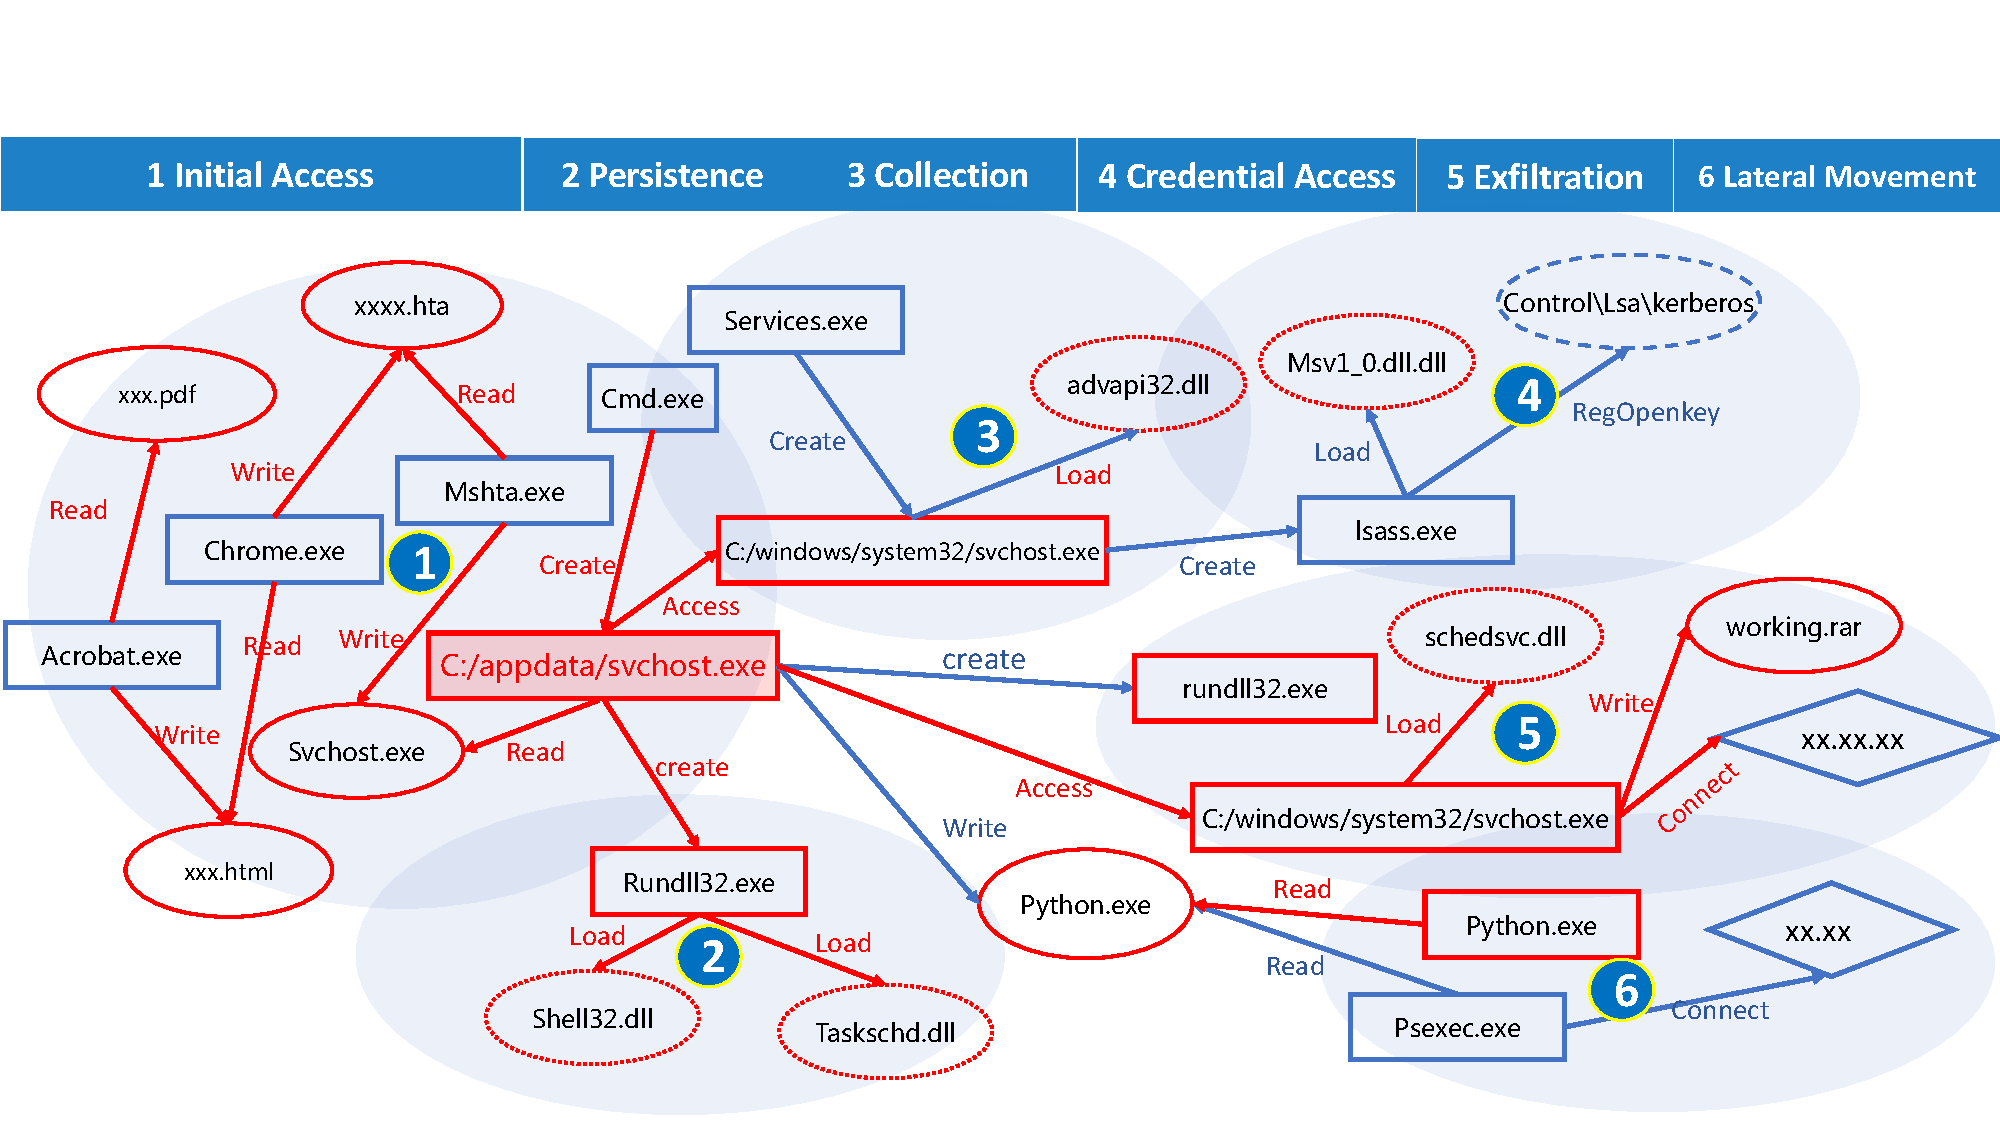
\includegraphics[width=0.95\textwidth]{figs/example.pdf}
    \caption{ 
    System entities are represented by nodes in the graph. 
    The attack-relevant elements are highlighted in red, while those representing regular events and nodes are displayed in blue.
    Processes, file-type entities (dlls, registry, files, etc.), and sockets are represented by rectangles, ovals, and diamonds. Solid line ovals represent files, dashed line ovals represent registries, and dotted line ovals represent DLLs.A series of operations is represented by an edge, such as a read, a create, a load, etc. We have segmented the attack progression into six distinct steps using a light blue backdrop. }
    \label{fig-example}
    \end{figure*}

\paragraph{Attack Scenario}
Figure~\ref{fig-example} illustrates a simplified provenance graph derived from audit records of a trojan-induced APT attack. System entities are represented by nodes in the graph. 
Processes, file-type entities (dlls, registry, files, etc.), and sockets are represented by rectangles, ovals, and diamonds. Solid line ovals represent files, dashed line ovals represent registries, and dotted line ovals represent DLLs.
A series of operations is represented by an edge, such as a read, a create, a load, etc.
There are 6 steps that are followed in the trojan-induced APT attack.
%In our analysis of APT attack reports \cite{eclecticiq2023,microsoft2023,paloaltonetworks2023}, we identify common attack steps and stealthy methods, such as Process Masquerade, Process Injection, Process Hollow, and DLL-Side Loading\cite{eclecticiq2023}. As a result of the use of four common obfuscation techniques, we were able to assemble ten scenarios for APT attacks using 23 malicious functions disguised as DLLs and program names.
%One of attack scenario as motivating example is used to illustrate current detection methods' limitations as well as our approach's intuition.


\begin{enumerate}[leftmargin=*]
    \item Initial Access: The attacker first sends the victim a malicious pdf file \textit{xxx.pdf} that contains a virus. Unfortunately, the application \textit{Acrobat.exe} that reads PDF files does not protect against the malicious code that is hidden inside the document. As a result, the malicious code downloads the malicious \textit{xxxx.hta} file, and the malicious program \textit{svchost.exe} is then downloaded and executed within the directory \textit{c:/appdata/svchost.exe}.
    \item Persistence: As an attempt to hide itself, this malicious \textit{C:/appdata/svchost.exe} opens \textit{rundll32.exe}, which then uses a DLL Side-Loading technique to load a malicious DLL \textit{shell32.dll}, which contains functionality for establishing persistence in the compromised system.
    \item Collection: Malicious \textit{C:/appdata/svchost.exe} then injects malicious \textit{advapi32.dll} processes into a benign \textit{C:/windows/system32/svchost.exe} and uses the malicious dll disguised as \textit{advapi32.dll} to gather information.
    \item Credential Access: Meanwhile, by exploiting a vulnerability, the attackers downgraded Kerberos to the more vulnerable NTLM protocol (\textit{Msv1\_0.dll}). In order to move lateral within the network, they stole credentials from the domain.
    \item Exfiltration: A malicious attacker hollows out a portion of the memory space of the benign process svchost, fills it with malicious programs, and packages up the information into a ZIP file known as \textit{working.rar}.
    \item Lateral movement: After obtaining the credentials from step 4, the attacker executed the renamed \textit{python.exe} file, thus gaining lateral access to the network.
\end{enumerate}




%\paragraph{Challenges to Existing Solutions}
%Our simulated APT attack shows the following limitations of provenance-based threat detection:
%\begin{itemize}[leftmargin=*]
%    \item \textit{Misuse-based Detection}:  A misuse-based detector\cite{milajerdi2019holmes,milajerdi2019poirot} detects cyber threats by matching audit records with security policies that describe attack semantics. The creation of these security policies is time-consuming and requires domain knowledge, even though such detection maintains a low false-positive rate. As shown in our example, a single TTP can correspond to a variety of different attacks, while "initial access" can be implemented in a variety of ways, our case utilizing \textit{Mshta.exe}. It is the responsibility of experts to cover all attack behaviors for a given TTP, but this is a time-consuming and labor-intensive process, and it cannot handle unknown or evolving threats. In addition, experts' subjective interpretations of attacks, varying proficiency levels, or even human error can affect the quality of policy formulation.
%    \item \textit{Anomaly-based Detection}: Anomaly-based detection techniques detect deviations, but they rarely provide a deeper understanding of the underlying attack mechanisms. Identifying the root cause of this attack scenario can be difficult due to the deluge of records generated by this attack scenario. As an example, Unicorn\cite{han2020unicorn} may trigger alerts across a graph, but it cannot pinpoint which particular entities or patterns are triggered. As a result of their ability to mimic benign activities, they are practically imperceptible, and in this attack scenario, many disguised behaviors can be seen. Process hollow is one of the disguised behaviors used in step 5. We get \textit{rundll32.exe} and the malicious \textit{svchost.exe} using the same vector based on Shadewatcher\cite{zengy2022shadewatcher}, so we cannot detect exceptions. Furthermore, the number of anomalous entries in benign logs is very low (less than 1\% of all entries are malicious). The limited representation of stealthy threats in logs makes it difficult to train a robust and reliable model.
%    \item \textit{Statistics-based Detection}: Even though statistics-based approaches \cite{liu2018towards,hassan2019nodoze,hassan2020we} identify potential threats within graphs, they often misinterpret benign but rare threats. For instance, in our motivating example, svchost has many functions, one of which hosts the schedule service. False alarms can occur due to infrequent incidents being flagged as attacks.
%\end{itemize}
%All of these methods have difficulties in identifying attacks in a timely and accurate manner. Further, they do not provide sufficient granularity to clarify and explain specific attack behaviors, which complicates the identification and response process in the event of an attack.



\paragraph{Our Solution}
\label{sec:intuition}
%As we mentioned previously, we analyze numerous APT attack
%reports\cite{eclecticiq2023,microsoft2023,paloaltonetworks2023} and discovered that attackers often employ disguise techniques to hide their malicious activities.
%The techniques include Process Masquerade, Process Injection, Process Hollow, and Direct Loading.
%It is generally true that as attackers progress from straightforward masquerading techniques, like mimicking legitimate processes, to more sophisticated ones, such as DLL\-side loading, the stealthiness of their disguises tends to increase.

In spite of the masquerading method, there are inherent constraints associated with genuine program behavior, regardless of the disguised method - execution paths, parent-child relationships, permissions, as a process must execute operations, some of which must be performed in sequence, etc. Specifically, we have the following behaviorial invariants:

\fbox{
\linyun{TODO: $p_1 \land p_2 \land ... $}
}

However, there were significant deviations from these constraints. 
While \textit{svchost.exe} is typically spawned by \textit{services.exe}, the malicious variant here is spawned by \textit{cmd.exe}. Additionally, its execution path was not what one might expect for an authentic \textit{svchost.exe}.
For more stealth attacks, like process injection as shown in step 3, a maliciously injected \textit{advapi32.dll} disrupts the expected sequence of events and violates the associated constraints. Thus, it is essential that profiles and constraints are taken into account as detection signals for regular processes in order to improve detection capabilities.


\fbox{
\linyun{TODO:  $p_1 \land p_2 \land ... \land q_1$}
}

\linyun{$q_1$ for the runtime behaviors}


\section{Threat Model}\label{sec:threatModel}
We assume that APT attacks launch attacks with the following features:

\begin{itemize}[leftmargin=*]
    \item \textbf{Stealthy}. The attacker employs covert tactics, concealing their malicious activities amid a substantial volume of benign background data, resulting in the victim system exhibiting behavior akin to a benign mode.
    \item \textbf{Evolving}. Professional attacker groups continually innovate, extending their targets to a broader array of system processes and adeptly adjusting to the latest defensive mechanisms to maintain a competitive edge.
    %As professional attacker groups continue to innovate, they are targeting an ever-expanding range of system processes and adapting to the latest defensive measures in order to stay ahead of the game.
    \item \textbf{Frequent usage of zero-day exploits}. The attacker primarily relies on zero-day exploits, resulting in a lack of advance knowledge w.r.t. the specific attack patterns.
\end{itemize}

\section{Methodology of \tool}

\begin{figure*}[ht]
    \centering
      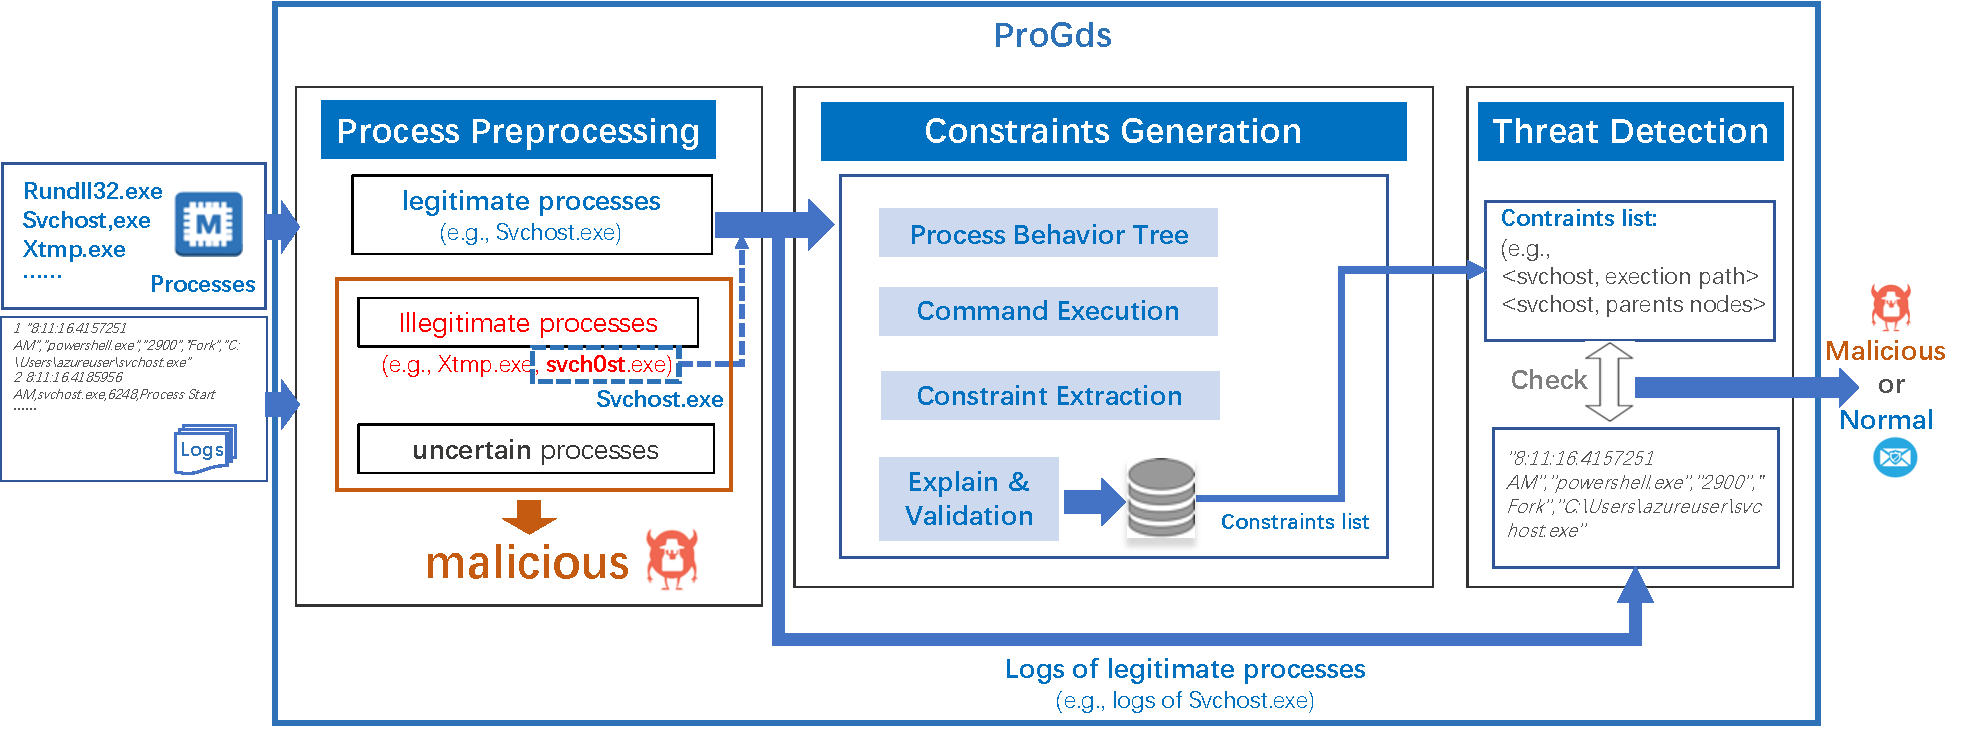
\includegraphics[width=0.95\textwidth]{figs/overview.pdf}
      \caption{An overview of \tool.}
    % \caption{The system process logs are collected and categorized using LLM as legitimate, illegitimate, and uncertain processes. Processes labeled uncertain or illegitimate are flagged for security analyst review (detailed in Section~\ref{sec:classifition}). If determined to be legitimate, LLM assists in the creation of a database of process constraints. This is achieved through behavior tree creation, command execution, constraint extraction and validation (explained in Section~\ref{sec:profile_con}). Logs that violate these constraints are indicative of potential threats (detailed in Section~\ref{sec:Threat_detection}).}
    \label{fig-framework}
    \end{figure*}


% Note that, as an alternative to sample-focused analysis, we propose to observe ubiquitous OS kernel processes. The system processes are always present and do not need to be identified before analysis, unlike suspicious samples.

\subsection{Technical Challenges}\label{sec:challenges}
A straightforward idea is to utilize the knowledge extraction capabilities in LLMs to facilitate the construction of more comprehensive profiles and constraints for victim system processes first, which can then be employed for conducting further thorough attack detection analysis. Recall that,
when dealing with the evolution of attacks or their stealthy tactics, supplemental knowledge can be very crucial. Moreover, in contrast to learning-based detection methods, this approach obviates the requirement for pre-defined attack patterns, which also enhances its adaptability and versatility in addressing evolving threat landscapes.
%How can we efficiently extract these constraints? It's a crucial question. Fortunately, LLMs offers significant advantages when it comes to building process profiles due to its exceptional knowledge extraction capabilities.
However, the direct employment of LLMs in our setting gives rise to the following three notable technical challenges:

% \circled{1} Complexity Handling: It might be difficult for LLMs to give comprehensive solutions when they are faced with complicated questions or scenarios.

\noindent
{\bf CH-\circled{1} Context Dependency.} %  :
To achieve precise outcomes, LLMs commonly necessitate an enriched contextual environment. In the absence thereof, their responses may exhibit a propensity towards generality or imprecision. However, ... \yd{YD: Add statement about "hardness in our setting to get enriched context environment directly"}

\noindent
{\bf CH-\circled{2} Memory Limitations.} % \circled{2}
\yd{YD: Add statement about facts w.r.t long context in our setting.} However, owing to the constraints imposed by their token limits, LLMs encounter challenges when confronted with exceedingly lengthy texts. Moreover, LLMs exhibit a proclivity for prioritizing recent interactions, often at the expense of overlooking pertinent details embedded within the broader context of prior conversational history.
% Due to its token limit, LLMs cannot handle excessively long texts. In addition, LLMs tend to focus more on recent interactions and overlook previous details in a conversation history.

\noindent
{\bf CH-\circled{3} Hallucination Problems.} % \circled{3}
In spite of the remarkable advancement of LLMs in excelling across a diverse spectrum of understanding tasks, these intelligent models still show a significant drawback: the tendency to `hallucinate', i.e., they may generate misinformation and lead to unsafe behaviors.\yd{YD: Add refers about Hallucination.}
% This risk entails
In this work, such a risk entails the possibility of the model generating information for a given system process that appears plausible at first glance but lacks factual support or corresponds to non-existent realities.
% that might reveal plausible-looking yet factually unsupported or nonexistent information if the model does produce hallucinations.

% Therefore, the key to building process profiles using LLMs is overcoming these challenges which is the central focus of this paper.

\subsection{Overview of \tool}
In this work, we propose an effective LLMs-based APT attack detection framework, named \tool, addressing all the above challenges. The overview of \tool can be found in Figure~\ref{fig-framework}.

\tool comprises three main components: Process Preprocessing, Constraints Generation, and Threat Detection.
Given a bundle of logs collected from a variety of system processes, \tool first conducts an LLMs-based process preprocessing procedure to filter out processes with legitimate names and transmit these names into the Constraints Generation component, while concurrently forwarding the detailed logs of the legitimate processes to the Threat Detection component. Note that, in cases where illegitimate processes share names resembling those of legitimate counterparts, \tool not only identifies and corrects them but also categorizes them as legitimate processes. For other illegitimate or uncertain processes, \tool classifies them as potentially malicious ones. Then, the LLMs-based Constraints Generation component constructs a database for all the legitimate processes received from the previous step, outlining the typical constraints associated with the processes. Finally, the Threat Detection component checks the consistency between the constraints generated and the original logs, and any violation of these constraints will be indicated as a malicious activity.

To address the technical challenges outlined in Section~\ref{sec:challenges}, we decompose the Constraints Generation component into four LLMs-manageable subtasks.


% As illustrated in Figure~\ref{fig-framework}, we accessed a log collection tool to collect logs from a variety of system processes that were running at different times in the system. Utilizing the powerful capabilities of LLMs, we were able to categorize these processes based on their names into three distinct categories: legitimate process names, illegitimate process names, and uncertain process names (due to the inherent incompleteness of the GPT's database). As for the latter two categories, we classified them as potentially malicious, requiring more investigation by security analysts in order to determine whether they are malicious or not. A more in-depth examination of this process is provided in Section~\ref{sec:classifition}.

% As for processes that were classified with legitimate names, we used the LLMs to construct a database that outlined the normal constraints of the process.

% In a previous Section~\ref{sec:intuition}, we briefly discussed the four challenges that exist when building process profiles based on the LLMs model. To address these challenges, we developed ProfileGuard, a method that harnesses LLMs for the automated creation of critical system process profiles based on the information provided by LLMs. ProfileGuard acts as a security guard for the system, using system process profiles to prevent malicious attackers.
% We broke down the comprehensive profiling task into four manageable subtasks:
\noindent
{\bf Process Behavior Tree Construction.} To provide an enriched contextual environment for LLMs, we first capture a comprehensive range of behaviors for each process, i.e., creating a behavior tree for each process. Then, the Large Language Model (LLM) continuously expands its knowledge of this behavior tree through a ``self-ask" manner. Finally, the LLM benefits greatly from this behavior tree as it provides an enriched contextual environment, which can greatly tackle the challenge {\bf CH-\circled{1}}.

\noindent
{\bf Command Execution.} The behavior tree can then be used to guide the LLMs to script and execute commands for behaviors that could be addressed. In addition, command execution generates richer contextual information for {\bf CH-\circled{1}}, and checks simple constraints, such as execution paths and parent-child relationships. \yd{YD: Recheck and Refine.}

\noindent
{\bf Constraint Extraction.} In this step, we'll combine the LLMs and traditional programs to solve {\bf CH-\circled{2}}. Since the log size is large, asking GPT directly will easily exceed its memory limit and cause previous information to be lost. We employed common term and prefix-span sequence mining to discover deeper relationships between logs. Each constraint, which was identified by LLMs, was interpreted using its knowledge. \yd{YD: Recheck and Refine.}

\noindent
{\bf Explanation \& Validation.} LLMs must be accurate and consistent due to potential hallucination issues. We've implemented a two-tier validation approach to validate the model's outputs for {\bf CH-\circled{3}}. The first tier involves executing actual commands and cross-checking with real-world logs. Multiple LLMs engage in a multi-round debate to mutually verify their respective responses and reasoning, aiming to arrive at a unified conclusion. \yd{YD: Recheck and Refine.}
% \begin{itemize}
%     % \item \textbf{Process Behavior Tree Construction}: Our goal was to capture a comprehensive range of behaviors for each process, creating a behavior tree. Through a "self-ask" approach, the LLMs continuously expanded its knowledge of this tree. LLMs can benefit greatly from this tree as it provides context for {\bf CH-\circled{1}}.
%     % \item \textbf{Command Execution}: A behavior tree was used to guide the LLMs to script and execute commands for behaviors that could be addressed. In addition, command execution generates richer contextual information for {\bf CH-\circled{1}}, and checks simple constraints, such as execution paths and parent-child relationships.
%     % \item \textbf{Constraint Extraction}:  In this step, we'll combine the LLMs and traditional programs to solve {\bf CH-\circled{2}}. Since the log size is large, asking GPT directly will easily exceed its memory limit and cause previous information to be lost. We employed common term and prefix-span sequence mining to discover deeper relationships between logs. Each constraint, which was identified by LLMs, was interpreted using its knowledge.
%     \item \textbf{Validation}: LLMs must be accurate and consistent due to potential hallucination issues. We've implemented a two-tier validation approach to validate the model's outputs for {\bf CH-\circled{3}}. The first tier involves executing actual commands and cross-checking with real-world logs. Multiple LLMs engage in a multi-round debate to mutually verify their respective responses and reasoning, aiming to arrive at a unified conclusion.
% \end{itemize}

% Leveraging this process behavior database, we compared extracted log information against the established constraints. Any violation of these constraints is indicative of potential malicious activity.
% A detailed discussion on this topic is set out in Section~\ref{sec:Threat_detection}.







\section{Design of \tool}

\begin{figure*}[h]
    \centering
      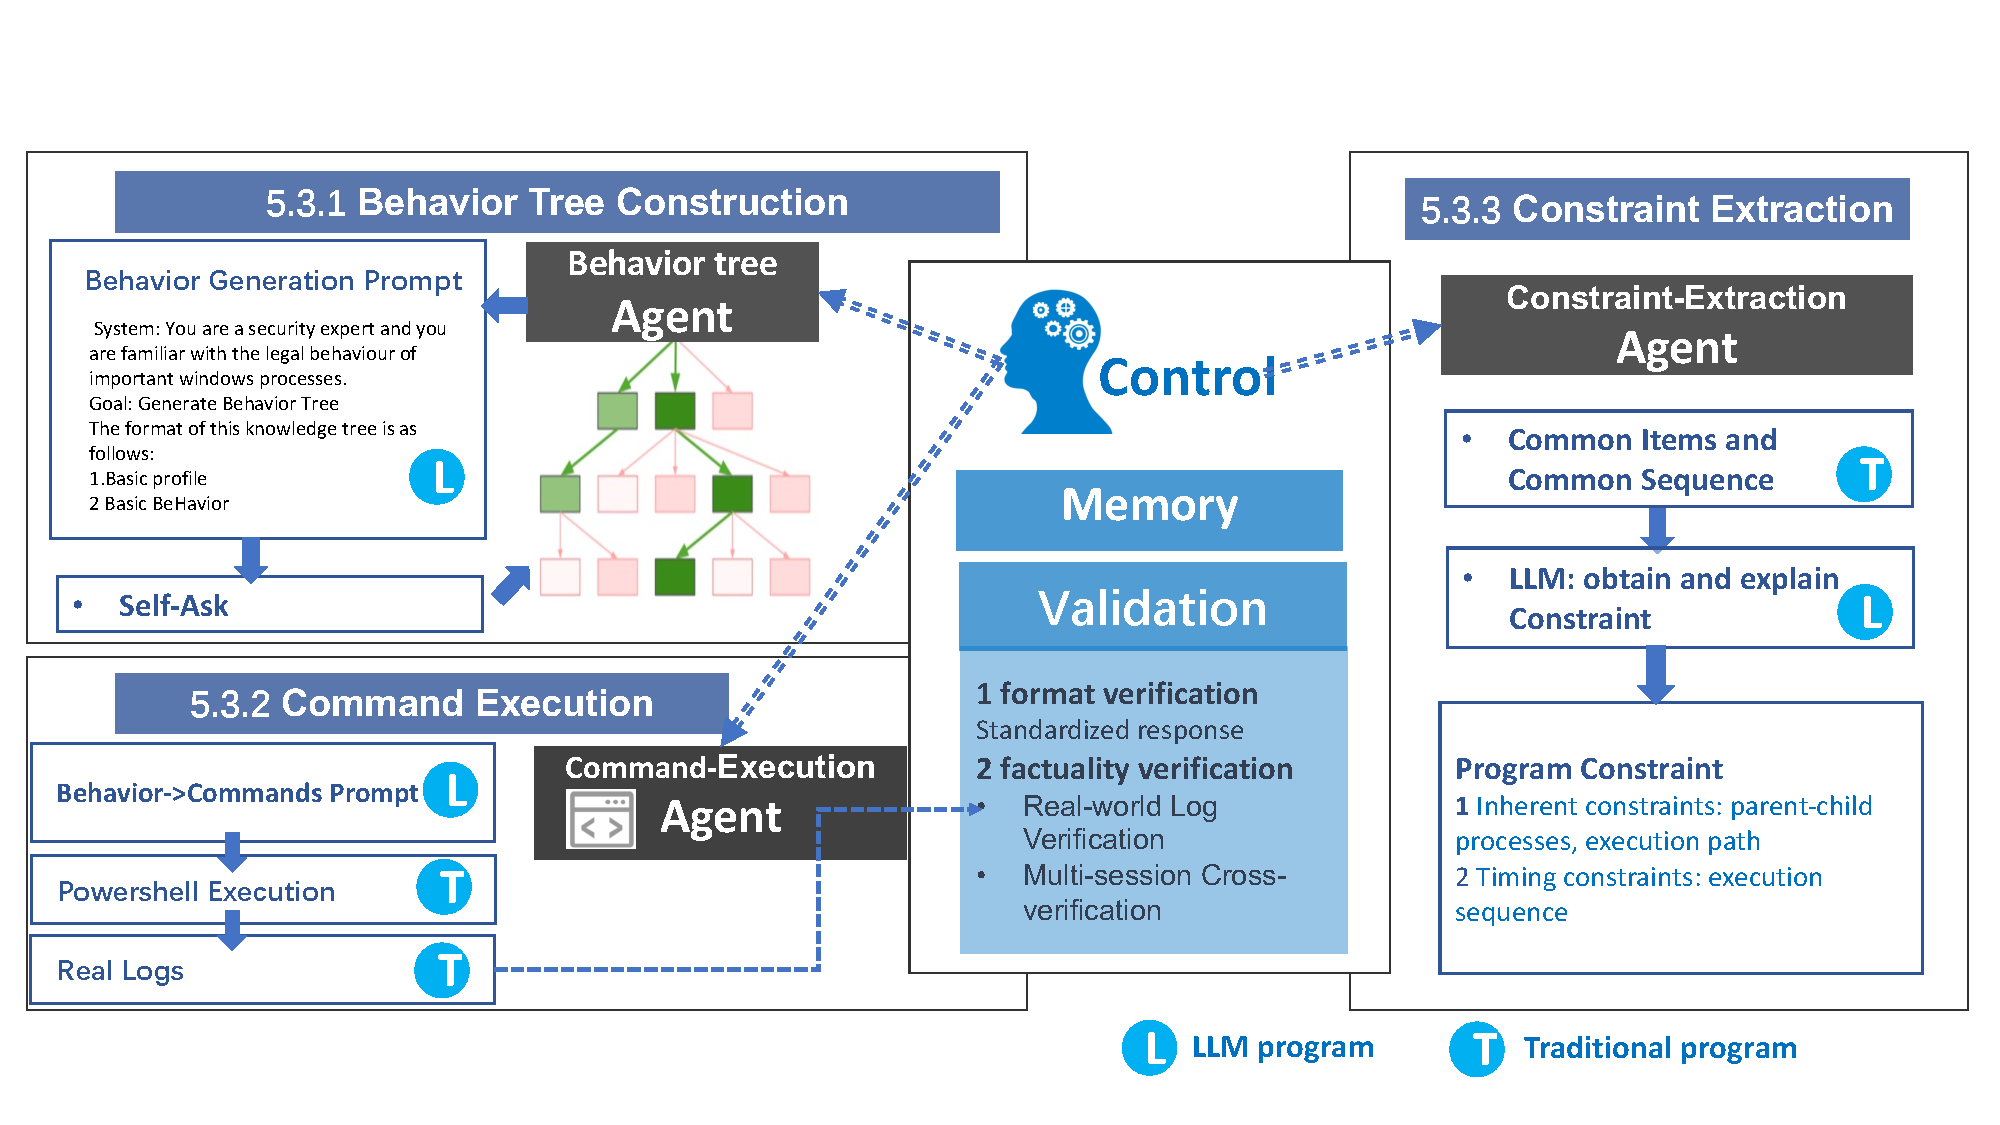
\includegraphics[width=0.9\textwidth]{figs/prompt.pdf}
    \caption{The system is controlled by a central "controller" with memory storage and validation capabilities. Our controller deploys three key modules: 1) Process Behavior Tree Construction Module, which maps out behavioral patterns; 2) Command Execution Module, which deploys active processes; and 3) Log Constraint Extraction Module, which determines log-based requirements. These units meticulously craft program profiles using LLMs-assisted strategies and traditional methods.}
    \label{fig-framework-prompt}
    \end{figure*}

\subsection{Definitions}

\subsubsection{System Entity and System Event}
We distinguish five principal entity categories: \textit{Processes}, \textit{Files}, \textit{Registry}, \textit{Dynamic Link Libraries (DLLs)}, and \textit{Network Connections}, the latter typically denoted by sockets. System entities possess unique attributes: the attributes associated with /textit[process] entities might include their Process ID (pid) or path to their executables. These entities' relationships and attributes are illustrated in Figure~\ref{fig-entity}. 

Our representation of a system event is given by
\[ e = (src, dst, rel, time) \]
where
\begin{itemize}
    \item \( src \) designates the source entity, constrained to only process entities,
    \item \( dst \) indicates the target or destination entity,
    \item \( rel \) describes their interaction nature, such as a process writing to a file,
    \item \( time \) specifies the timestamp of the event occurrence.
\end{itemize}
We also illustrated the temporal relationship between events as $\langle e_1 \to e_2 \to e_3 \rangle$, indicating that the events occur in a logical sequence. 



\begin{figure}[ht]
    \centering
      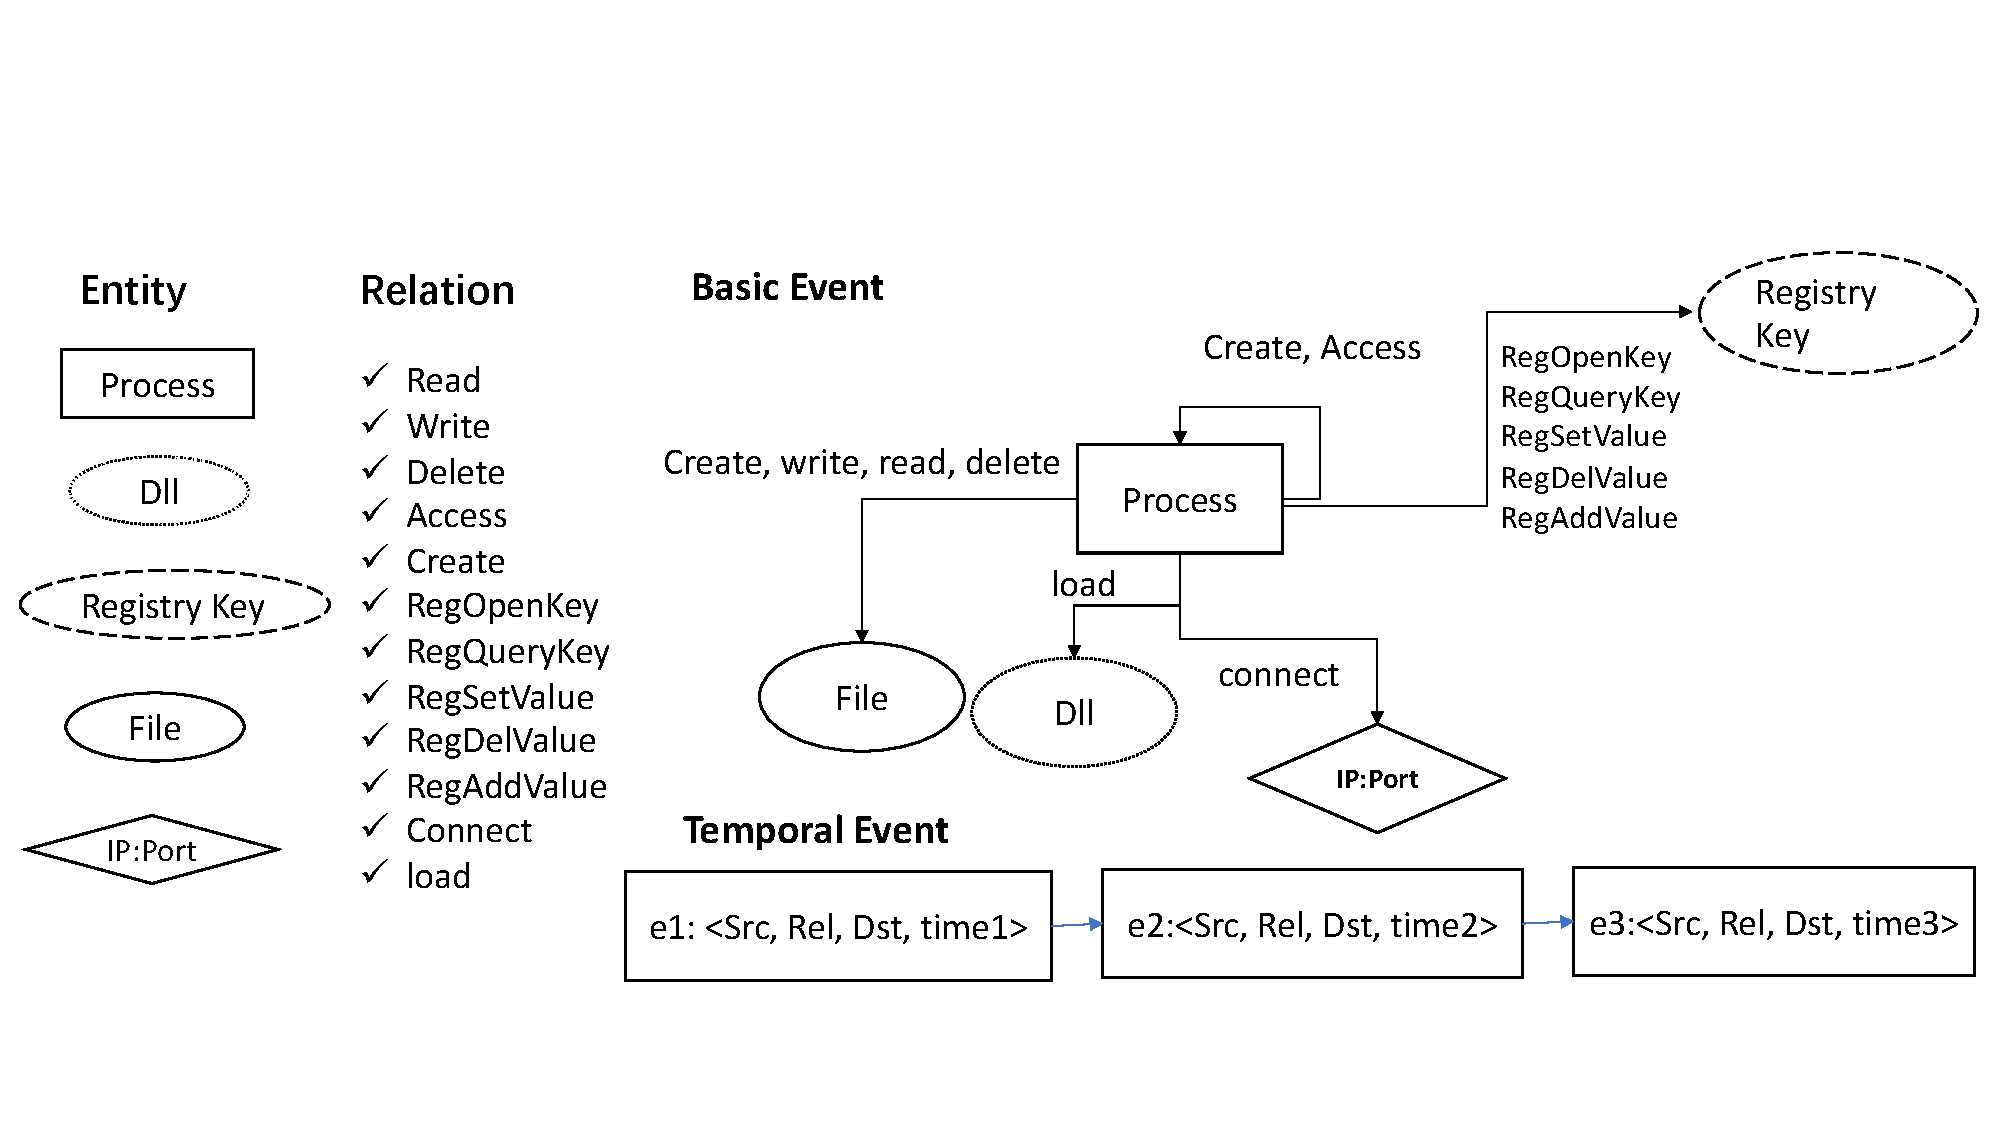
\includegraphics[width=0.45\textwidth]{figs/entity.pdf}
    \caption{System Entity and System Event.}
    \label{fig-entity}
\end{figure}

\subsection{Process Classification}

\subsubsection{Process Monitoring}

Process Monitoring is crucial: we need to gather logs from different processes in the system. In order to accomplish this, we use Windows' robust log collection and processing tool, Sysmon, to capture comprehensive system logs. Sysmon's default configuration ensures maximal log collection. 
However, due to the vast amount of logs, it becomes imperative to trim the data down. Using expert knowledge, we remove redundant and mundane events from the logs.

\subsubsection{Noisy Events Reduction}
Due to their inherent granularity and verbosity, audit logs introduce significant noise for analysts.
The omission of certain events does not impact the normal functioning of processes in behavioral cases. Integration of domain knowledge enhances our ability to reduce redundant events. There are also actions that are universal to all processes, such as loading \textit{ntdll.dll}  or \textit{kernel32.dll}. We've streamlined these ubiquitous events for a more concise representation.

\subsubsection{Process Classification}
\label{sec:classifition}
We created a prompt to query the LLMs about whether a particular program exists by name so that the classification could be completed. Using the LLMs' response, we classified these processes into three categories: legitimate process names, illegitimate process names, and uncertain process names (due to the incompleteness of the GPT database). In order to construct the profiles for the processes that fall under the legitimate category, we use the methods that are described in the sections that follow. The latter two categories should be investigated further by security analysts as they are potentially malicious.

\subsection{Profile Construction}
\label{sec:profile_con}
Next, we present our profile building module in detail, which consists of three agent components and a central program controller.
\tool is controlled by a central program controller, which is often referred to as the "brain" of the system. In this brain, two components are integral: memory and validation mechanisms, which include both format and factual verification. 
Format validation of LLMs results can be solved with simple traditional programs.

In order to conduct the factual validation, multiple LLMs sessions are debating each other, as well as real-life logs being validated.
This central program controller controls three distinct agent modules: the Process Behavior Tree Construction Module, the Command Execution Module, and the Log Constraint Extraction Module. Each module manages LLMs sessions and context independently, ensuring both coherence and specialized expertise. It combines LLMs-driven processes (like behavior tree construction) with conventional computational tasks (like frequent sequence mining). A combination of traditional and LLMs-driven processes is used to create detailed process profiles under program controller guidance.

\subsubsection{Process Behavior Tree Construction}
The construction of \textit{Process Behavior Trees} is one of the most important steps in the process.
First, we define the \textit{Process Behavior Tree}.
\begin{figure}[h]
    \centering
    \begin{subfigure}{0.45\textwidth}
      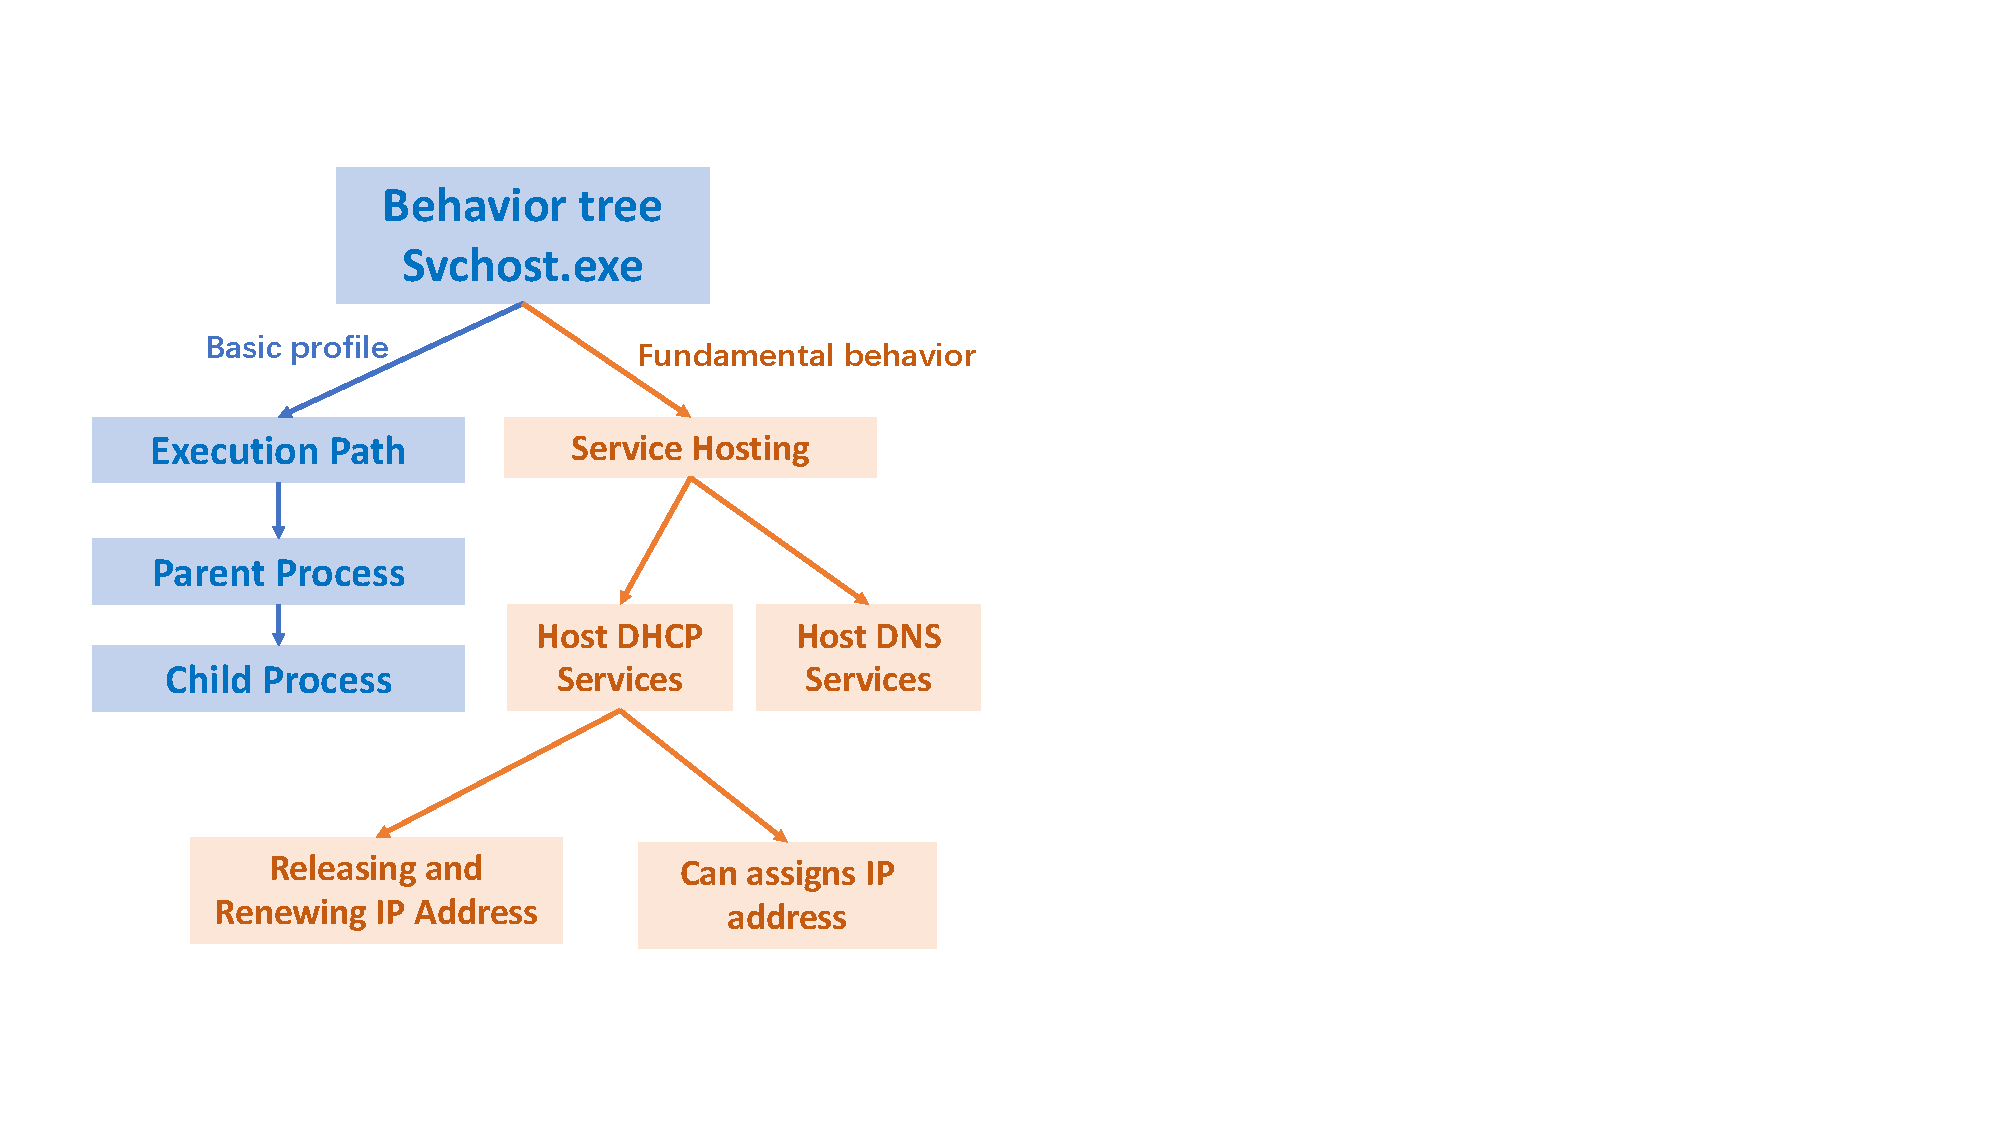
\includegraphics[width=1\textwidth]{figs/tree1.pdf}
      \caption{Process Behavior Tree Representation}
    \end{subfigure}
    \begin{subfigure}{0.45\textwidth}
    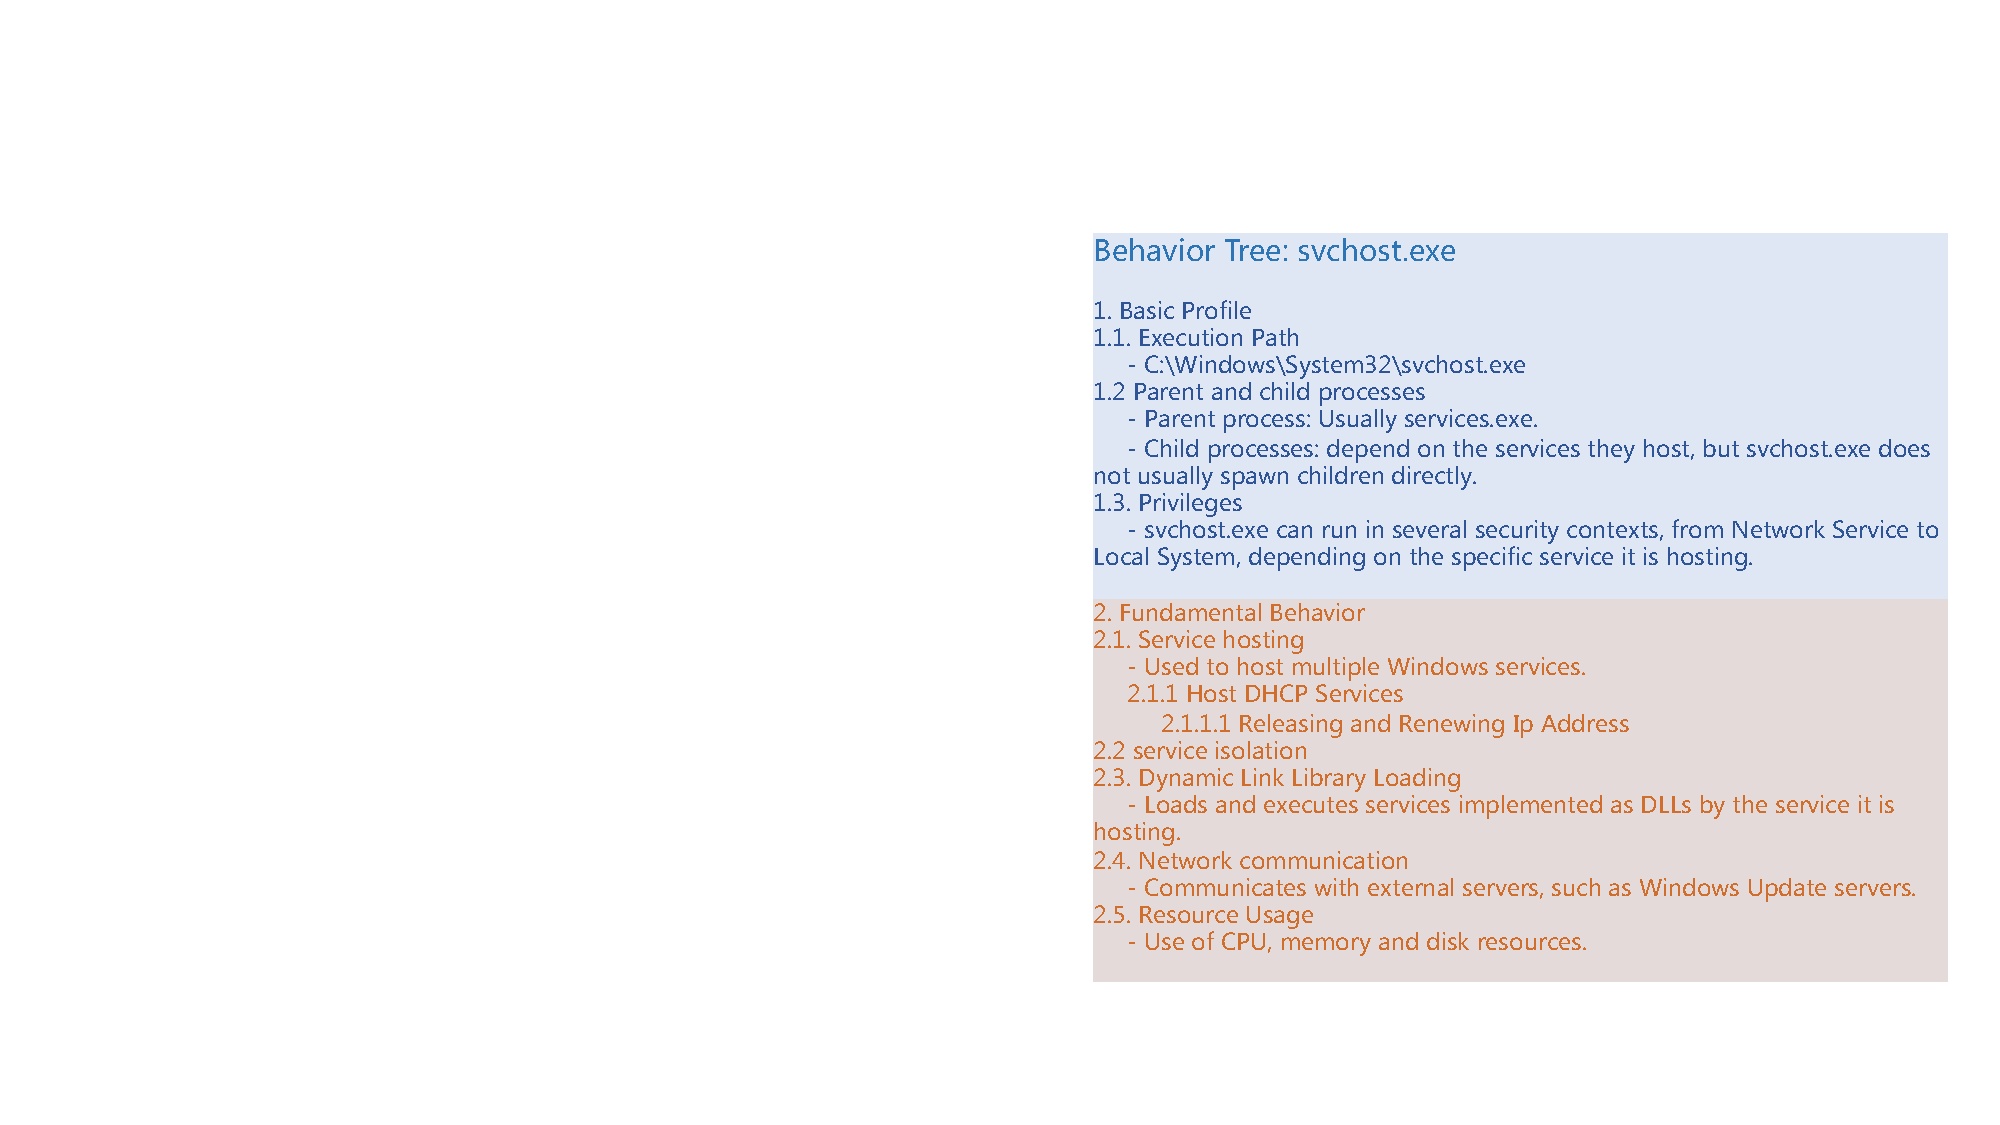
\includegraphics[width=1\textwidth]{figs/tree2.pdf}
    \caption{Process Behavior Tree Representation in natural Language}
    \end{subfigure}
    \vspace{-0.05in}
    \caption{In two formats: a) visualized tree format; and b) natural language format encoded in LLMs.}
    \label{fig:behavior-tree}
    \vspace{-0.15in}
    \end{figure}


\begin{definition}[Process Behavior Tree]
A Process Behavior Tree (BT) is a tuple \((N, B)\), where:
\begin{enumerate}
    \item \(N\) is a set of nodes organized in a tree structure. Each node represents legitimate behavior of a process. A node possesses a unique identifier within it, as well as a special node, called the root, which has no parent and does not contain any children. Except for the root of the tree, all nodes have exactly one parent and a zero number of children. There can be a sub-behavior associated with each of these children nodes.
    \item \(B\) is a function that assigns to each node \(n \in N\) a set of attributes \(B(n)\). Each attribute is a pair \((b, w)\), where \(b\) is the behavior name and \(w\) is a description or attribute of that behavior. 
\end{enumerate}
\end{definition}

To generate as many behaviors as possible, we've crafted two prompts: the "Initialization Behavior Tree Prompt" and the "Expansion Behavior Tree Prompt" (A detailed prompt can be found in the Appendix~\ref{prompt-init-tree}). Initially, we employ the Initialization Behavior Tree Prompt to create a foundational behavior tree. Subsequently, this tree is expanded through iterative rounds using the Expansion Behavior Tree Prompt. In order to create a diversity and precision of behaviors, we have incorporated four strategies:
\begin{itemize}
    \item Creating an Initial Process Behavior Tree: To ensure a standardized behavior tree, we've defined a specific output format for the behavior tree.
    \item Different Expansion Techniques in Behavior Tree Prompt: The Behavior Tree Prompt uses two distinct expansion techniques - self-ask and layer-wise. While self-ask aims at a macroscopic expansion of behaviors, layer-wise expansion delves deeper to uncover finer, detailed behaviors. To extract a comprehensive set of behaviors, these two methods combine breadth and depth searches.
    \item Conversation History and Language Learning Models: LLMs often ignore earlier details in a conversation, focusing on recent interactions. As a countermeasure, we leverage the benefits of the system role and embed both roles and objectives within it.
    \item Self-Evaluation by LLMs: We aim to provide LLMs with the ability to self-criticize and review current nodes. If the LLMs determines that the branch does not require expansion, node expansion is stopped.
\end{itemize}

The resulting behavior tree is illustrated in the Figure~\ref{fig:behavior-tree}. Taking the behavior tree of \textit{svchost.exe} as an example, we begin with the basic profile. This includes details such as the execution path of the process, its parent process (the parent process of \textit{svchost.exe} can only be \textit{services.exe}), and its child processes. Following this, we have the fundamental behaviors, such as service hosting, DLL loading, and service isolation exhibited by \textit{svchost.exe}. Focusing on the most significant behavior, which is service hosting, the behavior tree can be extended to detail the specific services being hosted. From the Figure~\ref{fig:behavior-tree}, one can observe the graphical representation of the behavior tree and its expression in natural language.




\subsubsection{Command Execution}

In this step, we design a prompt (detailed prompts can be found in Appendix~\ref{prompt-commands}) for generating commands based on a previous behavior tree. In order to obtain actual log files, this prompt generates corresponding system commands. We can verify some of the behaviors described in the previous step by collecting these logs. Using these logs, it is possible to directly verify some behaviors like parent processes, execution paths, and other details. It is, however, not possible to translate all system processes behaviors into executable commands. In these cases, we employ the LLMs to produce relevant recommendations, which guide us in manually engaging with the system to obtain the required logs.

\subsubsection{Constraint Extraction}

\begin{figure*}[h]
  \begin{subfigure}{.5\textwidth}
      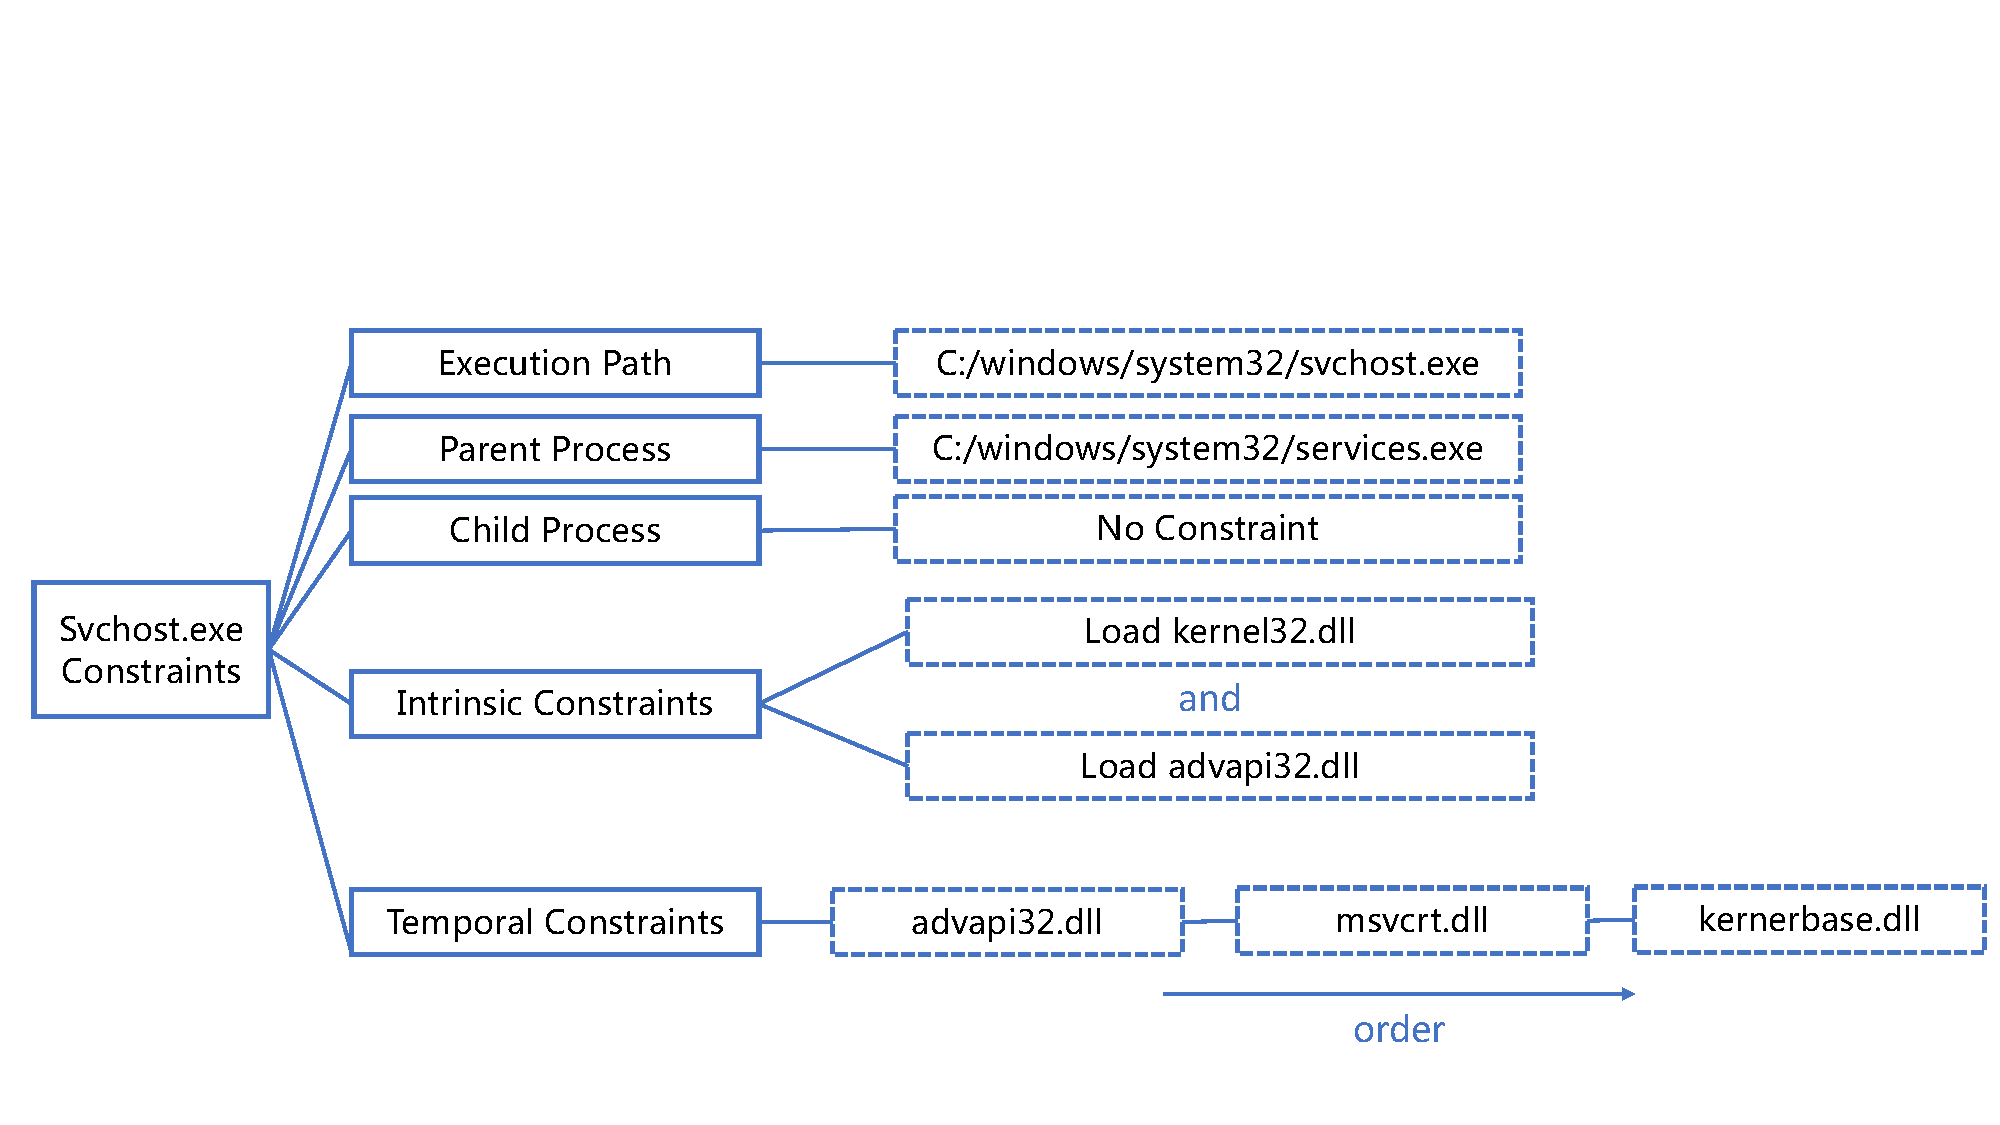
\includegraphics[width=\textwidth]{figs/svchost_constraints.pdf}
      \caption{Constraints of Svchost}
      \label{fig:cons-svchost}
  \end{subfigure}
  \hfill
  \begin{subfigure}{.5\textwidth}
      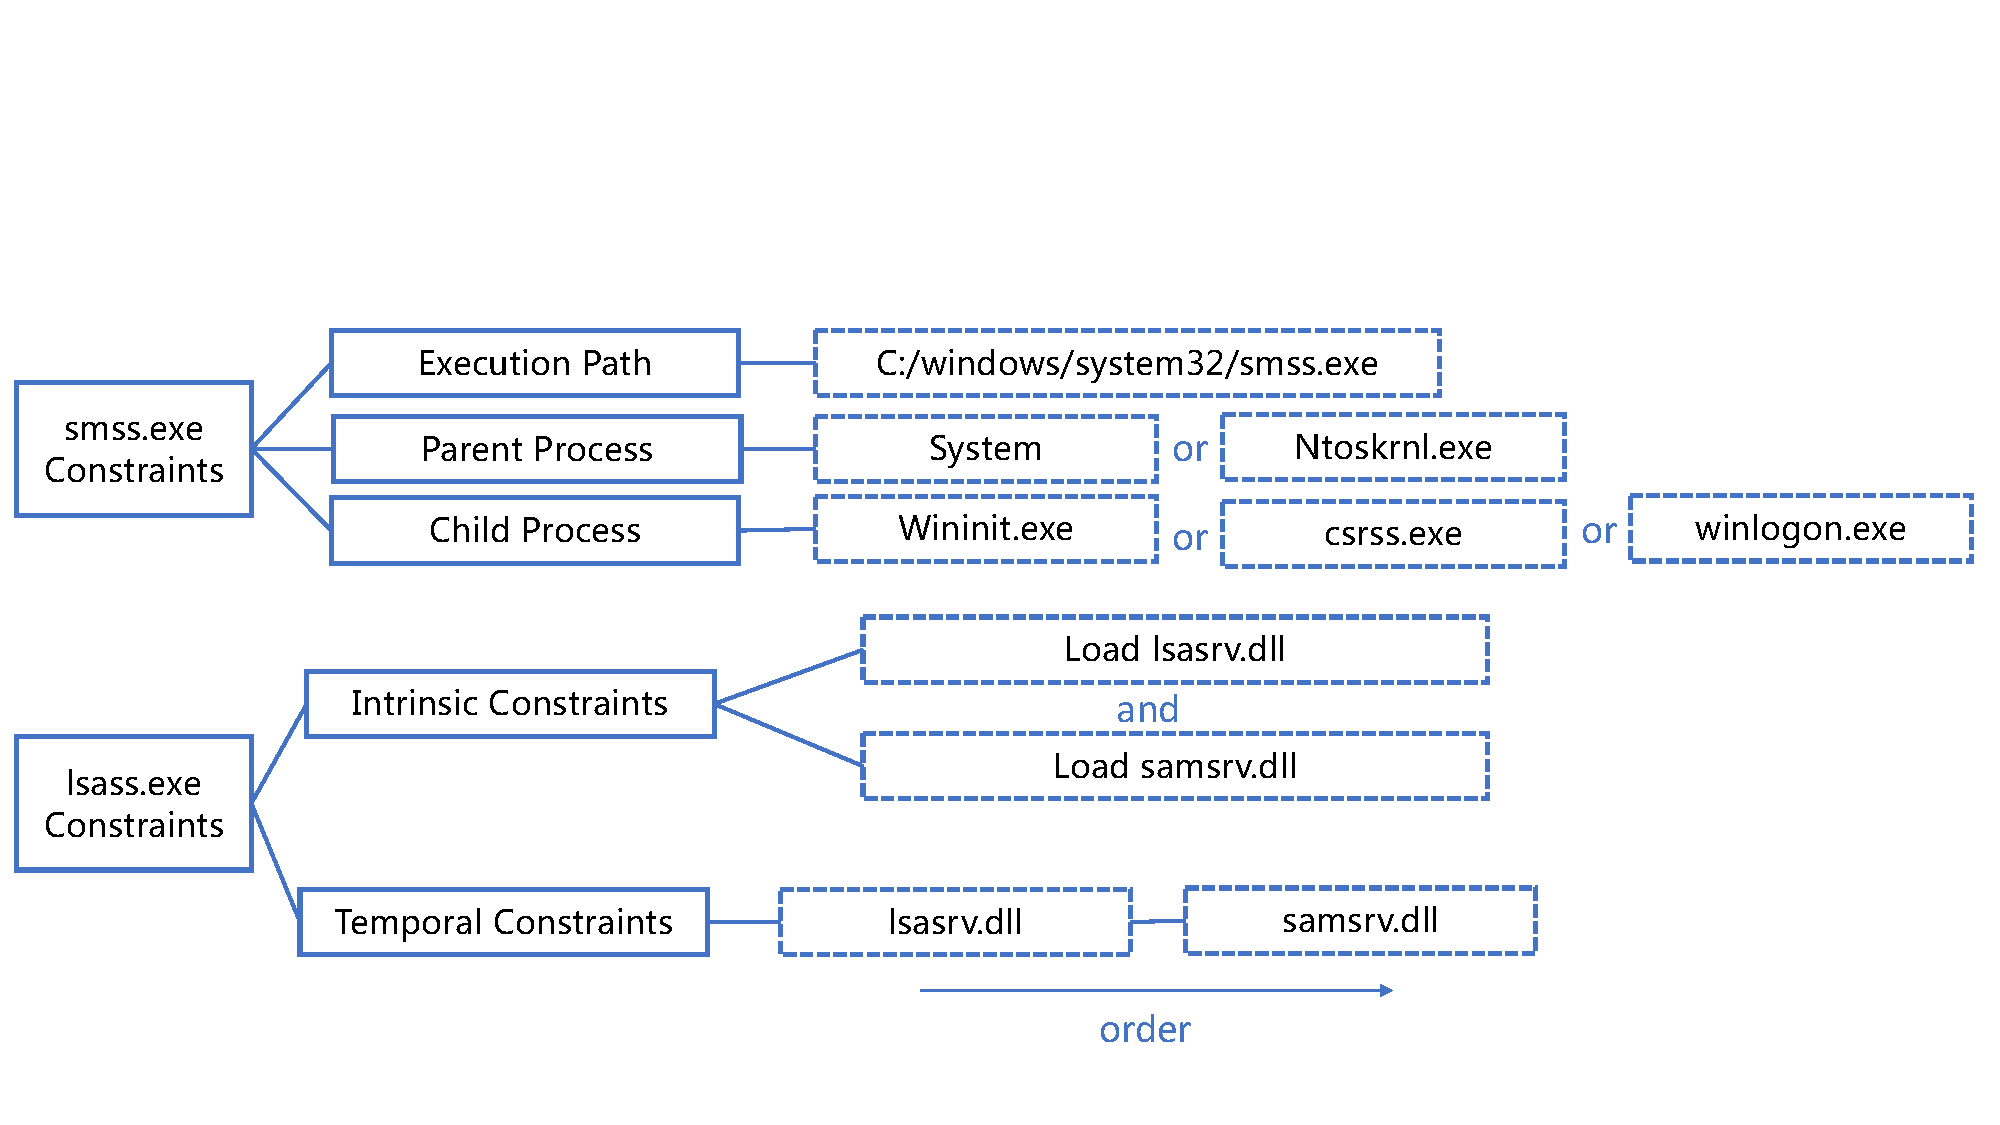
\includegraphics[width=\textwidth]{figs/smss_lsass_constraints.pdf}
      \caption{Constraints of Smss and Lsass}
      \label{fig:cons-smss-lsass}
  \end{subfigure}

  \begin{subfigure}{.5\textwidth}
      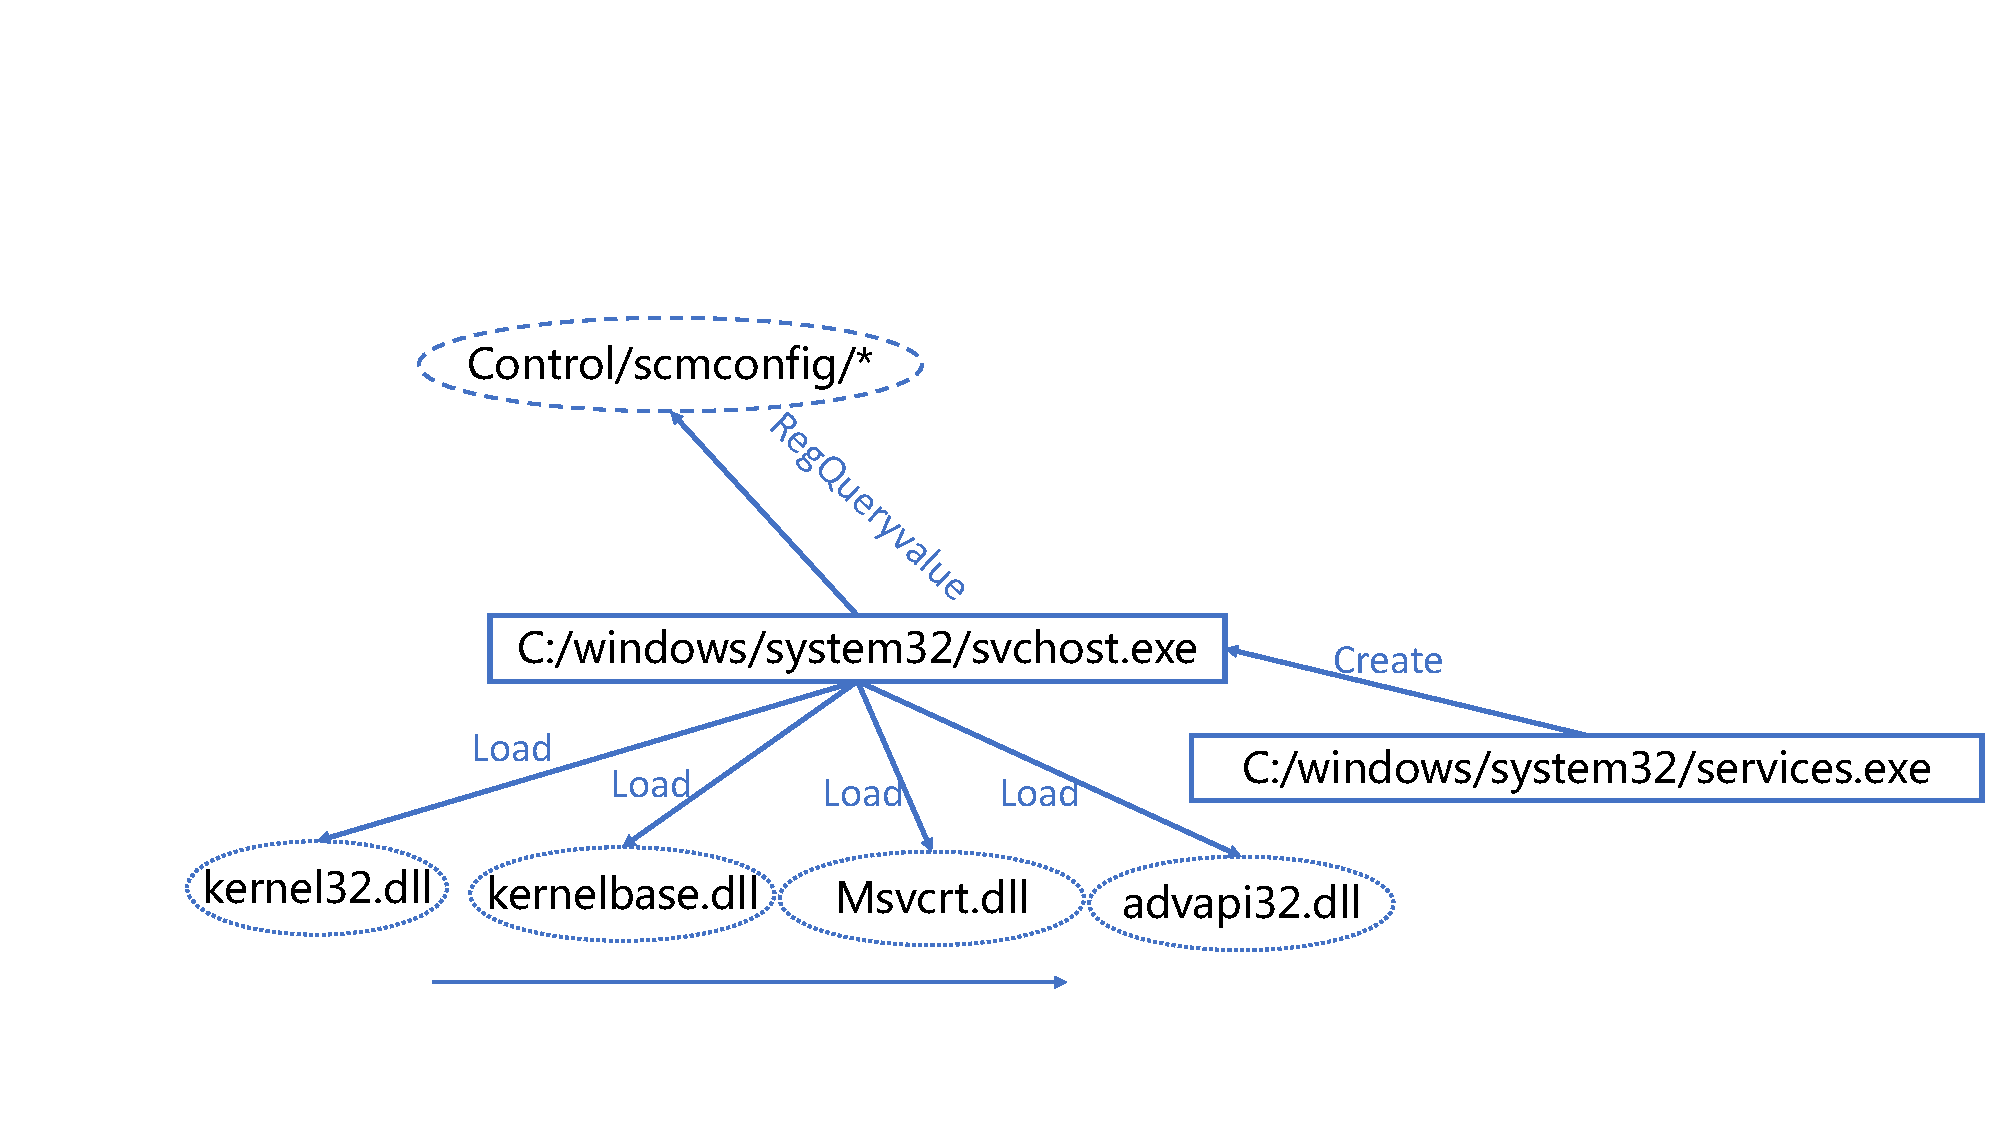
\includegraphics[width=\textwidth]{figs/svchost.pdf}
      \caption{Svchost Constraints in Graph format}
      \label{fig:con-svchost-tree}
  \end{subfigure}
  \hfill
  \begin{subfigure}{.5\textwidth}
      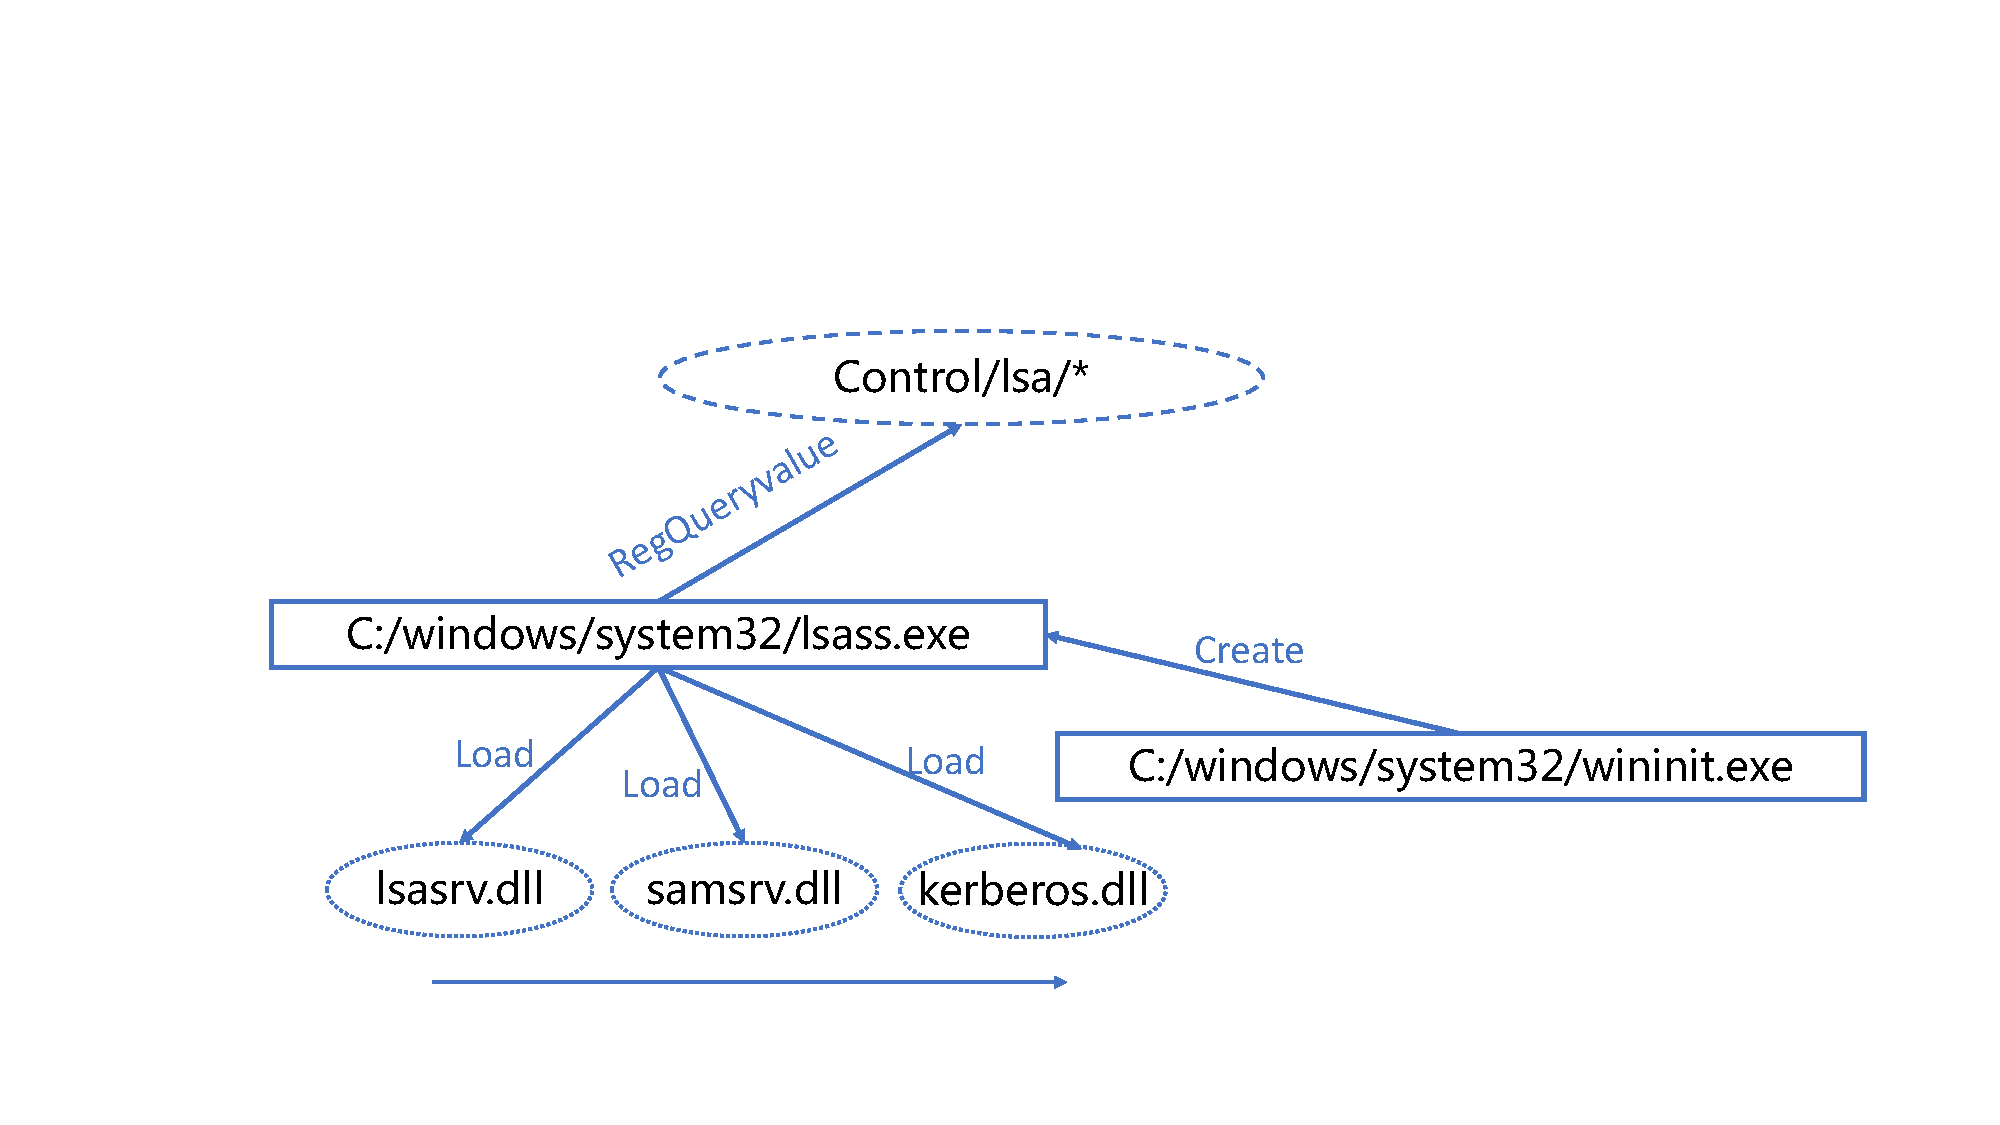
\includegraphics[width=\textwidth]{figs/lsass.pdf}
      \caption{Lsass Constraints in Graph format}
      \label{fig:con-lsass}
  \end{subfigure}
  \caption{Constraint Definition}
  \label{fig:cons-def}
 \end{figure*}


The extraction of system constraints is a pivotal step in our methodology. We begin by categorizing constraints into five types as shown in Figure~\ref{fig:cons-def}.
The Figure~\ref{fig:cons-def} illustrates the constraints of three processes: svchost.exe, lsass.exe, and smss.exe. In Figure~\ref{fig:cons-svchost}, the constraints of svchost.exe are shown. There are five types of constraints: execution path, parent process, child process, intrinsic constraints (svchost.exe will always load kernel32.dll and advapi32.dll.), and temporal constraints (advapi32.dll, msvct.dll, and kernelbase.dll must be loaded in the specified sequence).
For certain processes, like smss.exe, parent and child processes are optional. The parent process of smss.exe can be system.exe or Ntoskml.exe.
In summary, these constraint relationships can be fully characterized using the AND, OR, and ORDER operators.

By comparing them with the logs gathered in the previous steps, we can verify and extract the first three constraints directly.
However, for intrinsic and temporal constraints, the challenge arises due to real-world logs' vastness. It is impractical to query the LLMs for each log due to memory constraints and its propensity to forget extended conversations. To overcome this, we designed a hybrid method that combines traditional programming techniques with queries to the LLMs to extract these two constraints.

To clearly describe the common items and frequent sequence mining algorithms, we first provide some definitions.
Given a set of log sequences \( \mathcal{D} \), each sequence \( S \in \mathcal{D} \) contains logs \( L \), where each log is a tuple \( L = (s, o, d,t) \) consisting of:
\begin{align*}
    s & : \text{Source process} \\
    o & : \text{Operation} \\
    d & : \text{Destination or object of the operation}\\
    t & : \text{time specifies the timestamp of the event occurrence}
\end{align*}

We are trying to find frequent subsequences \( \mathcal{F} \) exceeding a threshold \( \theta \), here \( \theta =1\), indicating items that should occur frequently
We begin by mining the logs for common items among different log sequences in order to speed up frequent item mining. Our next step is to use the PrefixSpan algorithm to find frequent subsequences in these logs.
(Algorithms are detailed in the Appendix~\ref{alg:fre-common}).
Having established the common items and sequences, we then direct our queries towards the LLMs, focusing specifically on these elements to extract intrinsic and temporal constraints. Furthermore, we request the LLMs to explain its findings, providing insights into these constraints.
The detailed set of prompts used in this process as shown in Appendix~\ref{prompt-cons-explain}.



\subsubsection{Validation}
Due to the potential for hallucinations or misleading results, it is imperative to ensure the accuracy and consistency of LLMs outputs. Due to this challenge, we developed a two-dimensional validation system.

\textbf{Format Validation.}
As a result of this initial step, the model's output adheres to a predefined structure. Using conventional programming methods, deviations are corrected to match the expected format.

\textbf{Factual Validation.}
A more important verification is the factual validation, which is designed to ensure that LLM's final output is accurate and consistent.

\begin{itemize}
    \item Real-world Cross-referencing: LLMs outputs are executed as real-world commands, and their results are cross-checked against real-world logs.
    \item LLMs Multi-session Debates: The LLMs engages in iterative debates in multiple instances. Their goal is to find a consensus on an answer that is both accurate and reliable by verifying each other's responses and reasoning. They cannot reach a consensus on actions that are not entirely correct by having multiple LLMs debate each other. For definitive behaviors, they can eventually come to an agreement. A more detailed description of our approach can be found in the Appendix~\ref{prompt-cross-validation}.
\end{itemize}



\subsection{Threat Detection}
\label{sec:Threat_detection}

This is the basis of our offline process for building individual process profiles. An initial query is made to LLMs in order to determine whether processes with obfuscated or random names exist online. The process is likely to be malicious if it does not exist. Our established methodology allows us to profile processes that exist but are not in our knowledge base.

An anomaly detection process is based on a multitude of rules derived from the preceding steps. In various attacks, these rules are specifically designed to pinpoint the exact constraints that have been violated. Process masquerading, for example, violates execution pathway and parent-child constraints, whereas process injection violates inherent and temporal constraints more often.

\textbf{Construction Unseen Process Profile.}
Observing whether profile incompletion occurs in a sandbox environment helps prevent profile incompletion. This method may reduce false alarms for benign interactions between system entities that were not observed during profile construction.
\section{Experiment Evaluation}

In order to validate the effectiveness of our approach, we simulated 4 stealthy techniques, 23 malicious functions attacks on 100 critical system processes and ten APT attack scenarios:

\begin{itemize}
    \item \textbf{Q1.} How well does our method work, and does it achieve a low false-positive rate and false-negative rate? ((§~\ref{sec-effective})
    \item \textbf{Q2.} What is the time it takes for our method to construct a profile for each process? What is the most time-consuming step in the three-step process profile creation? (§~\ref{sec-eff})
    \item \textbf{Q3.} How does the behavior diverge based on LLM, and how does the validation step optimize the outcome? (§~\ref{sec-ab-study})
    \item \textbf{Q4.} How can we validate the accuracy of these explanations using our method? (§~\ref{sec-explanation-val})
    \item \textbf{Q5.} Is it common for real-world APT attacks to disguise their processes in various ways? (§~\ref{sec-real-world})
\end{itemize}
All experiments are performed on a server with Intel Xeon E5-2620 v4 CPUs @ 2.10GHz, 64 GB physical memory, and an NVIDIA Tesla V100 GPU. The OS is Ubuntu 16.04.3 LTS.
We implemented our system by calling OpenAI's GPT-4 API with a temperature setting of 0.5.
We develop \tool in 3.53K lines of C++ code and 10K lines of Python code.
The C++ code in the project is utilized for the generation of malicious attacks, while the Python code is employed for data preprocessing, building process profiles, and threat detection.


\subsection{Implementation}
We present important technical details in the implementation.

\subsubsection{System Auditing Collection}
Although \tool can handle input from Linux and Windows systems, our evaluation focuses primarily on Windows events. Because most of our benign deployment environment consists of Windows-based hosts, and sophisticated malware is mostly designed for Windows platforms, this is largely due to the fact that we have a benign deployment environment. We use Sysmon, Windows' sophisticated log collection tool, to collect provenance data from these systems. System logs are captured thoroughly and exhaustively by leveraging Sysmon's default settings.

\subsubsection{Attack Datasets}

To address the challenges, we approached the problem from three distinct angles: expanding coverage of malicious functionalities and the ATT\&CK framework, employing advanced stealthy techniques, and simulating genuine APT attacks.

We executed our APT attack simulations in three steps:
\begin{itemize}
    \item  \textbf{Enhancing Malicious Functionalities:} In order to simulate a wider range of malicious activities, we handcrafted 14 malicious functions in C++, including BypassUAC, Encryption, File Monitor, Keyboard Monitor, and Privilege Escalation. In addition, we implemented nine different TTP attacks using well-known hacker utilities like Caldera. Using C++ and Caldera methodologies, we achieved 23 distinct malicious functions. APT attacks take place at various stages, including Initial Access, Privilege Escalation, Information Gathering, Defense Evasion, and ensuring Persistence.
    \item \textbf{Employing Stealth Techniques:} We incorporated four stealth methods: Process Masquerade, Process Hollow, Process Injection, and DLL Side-Loading. By combining these stealth techniques with the 23 malicious functionalities, a variety of attack variants can be created. Process Masquerade and Process Hollow hide malicious process names, while Process Injection and DLL Side-Loading hide malicious DLLs.
    \item \textbf{Simulating Real-world APTs:} In order to enhance the authenticity of our simulations, we developed ten APT attack scenarios based on an analysis of real-world Advanced Persistent Threat activities. During a controlled testbed environment, audit logs were produced. We crafted ten simulated APT attack narratives using the four stealth techniques from the second step and the 23 malicious functionalities from the first step.
\end{itemize}

\noindent
{\bf Real-world datasets.} Using real-world datasets, we aimed to validate the frequency of obfuscation techniques such as name masquerading in authentic APT attacks and associated malicious software; to this end, we collected publicly available APT attack simulation datasets alongside malware samples like CozyCar,  callium, and Kevin etc. which are known to employ techniques like name masquerading and process injection;  APT29 poses as \textit{python.exe}, \textit{rar.exe}, and \textit{accesschk.exe}; furthermore, they utilize DLL Side-Loading, specifically by loading a malicious \textit{mso.dll} file, with comprehensive details showcased in the subsequent Table~\ref{tab:real_world}. We will delve into the specifics of how we utilized real-world datasets to validate the efficacy of our approach in Section~\ref{sec-real-world}.

\noindent
{\bf Label.}
By using our knowledge of attack workflow, we manually label the ground truth of interactions through their relation to attacks, as we are aware of how attacks are executed.


\subsubsection{Normal Datasets}
To validate the false positive rate of our methodology, we sourced a publicly available benign dataset from GitHub\cite{evtx-baseline2022}. This dataset encompasses logs generated from routine user activities across various Windows operating systems, including Windows 7, Windows 10 and Windows 11. The logs from this dataset cover the 13/47/52 processes we use to construct process profiles.

\begin{figure}[h]
    \centering
      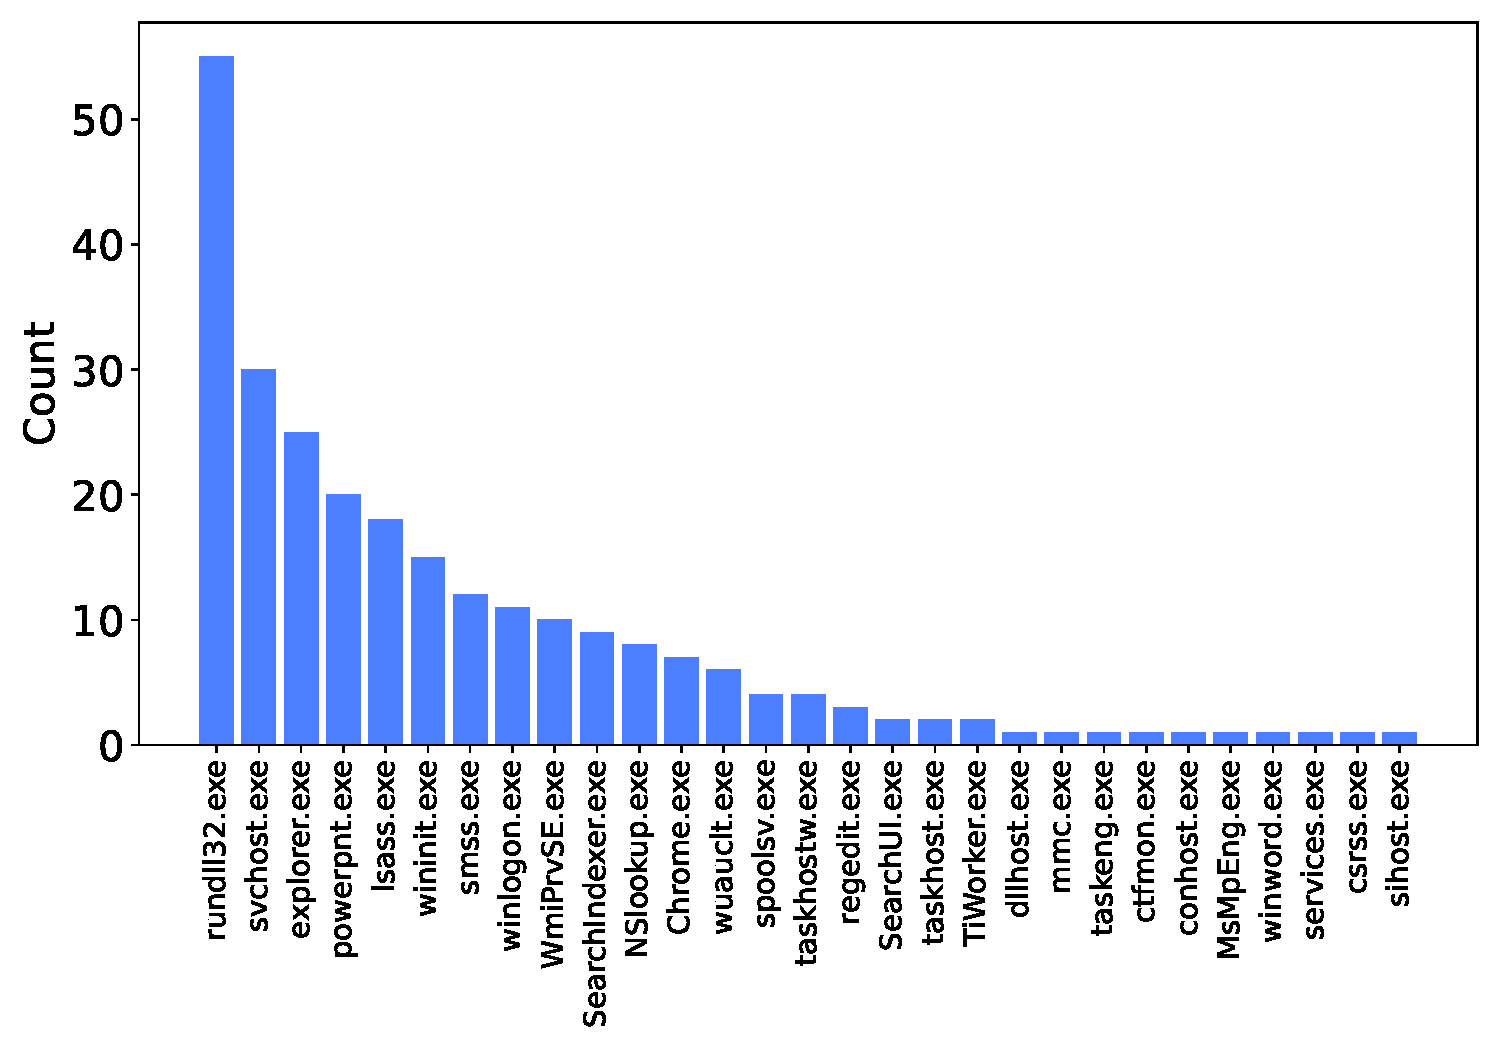
\includegraphics[width=0.45\textwidth]{figs/process.pdf}
    \caption{Comparison of attack frequencies for different processes based on the official MITRE website.}
    \label{fig-process}
\end{figure}

\subsubsection{Process Classification}

In order to construct a comprehensive analysis framework, we strategically selected 100 pivotal processes for examination. The selection criteria encompassed multiple dimensions, including: 1) Core system processes that are integral to system functionality; 2) Processes highly associated with security mechanisms; and 3) Processes commonly utilized by system administrators. Additionally, we integrated an assessment of processes that are frequently targeted in cyber-attacks, based on statistical analysis derived from MITRE's official website as shown in Figure~\ref{fig-process}


\newcommand{\colorbar}[1]{%
    \begin{tikzpicture}
        \definecolor{mycolor}{RGB}{255,204,204}
        \fill[mycolor] (0,0) rectangle (#1/100*0.7, 0.5); %0.7 is the width, adjust as needed
        \draw[black] (0,0) rectangle (0.7,0.5);
    \end{tikzpicture}
}


We highlight the two most common processes: svchost.exe and rundll32.exe:
\begin{itemize}
    \item \textbf{\textit{Svchost.exe} processes}. svchost.exe is a Windows system utility that runs multiple services from dynamic link libraries (.dll files). Given its trusted status and constant presence, adversaries often mimic svchost.exe for attacks. The behavior tree for svchost.exe, constructed based on our approach, is shown in the Figure~\ref{fig:behavior-tree}.
    \item \textbf{\textit{Rundll32.exe} processes}. \textit{rundll32.exe} loads specific functions from .dll files. Unlike \textit{svchost.exe}, it's more vulnerable, as attackers can create their own .dll for it. Due to its exploitability, \textit{rundll32.exe} is a prime target for malware impersonation. 
\end{itemize}



\subsection{Effectiveness}
\label{sec-effective}

\begin{figure*}
  \centering
  \begin{minipage}[b]{0.65\textwidth} 
  \begin{subfigure}{.5\textwidth}
      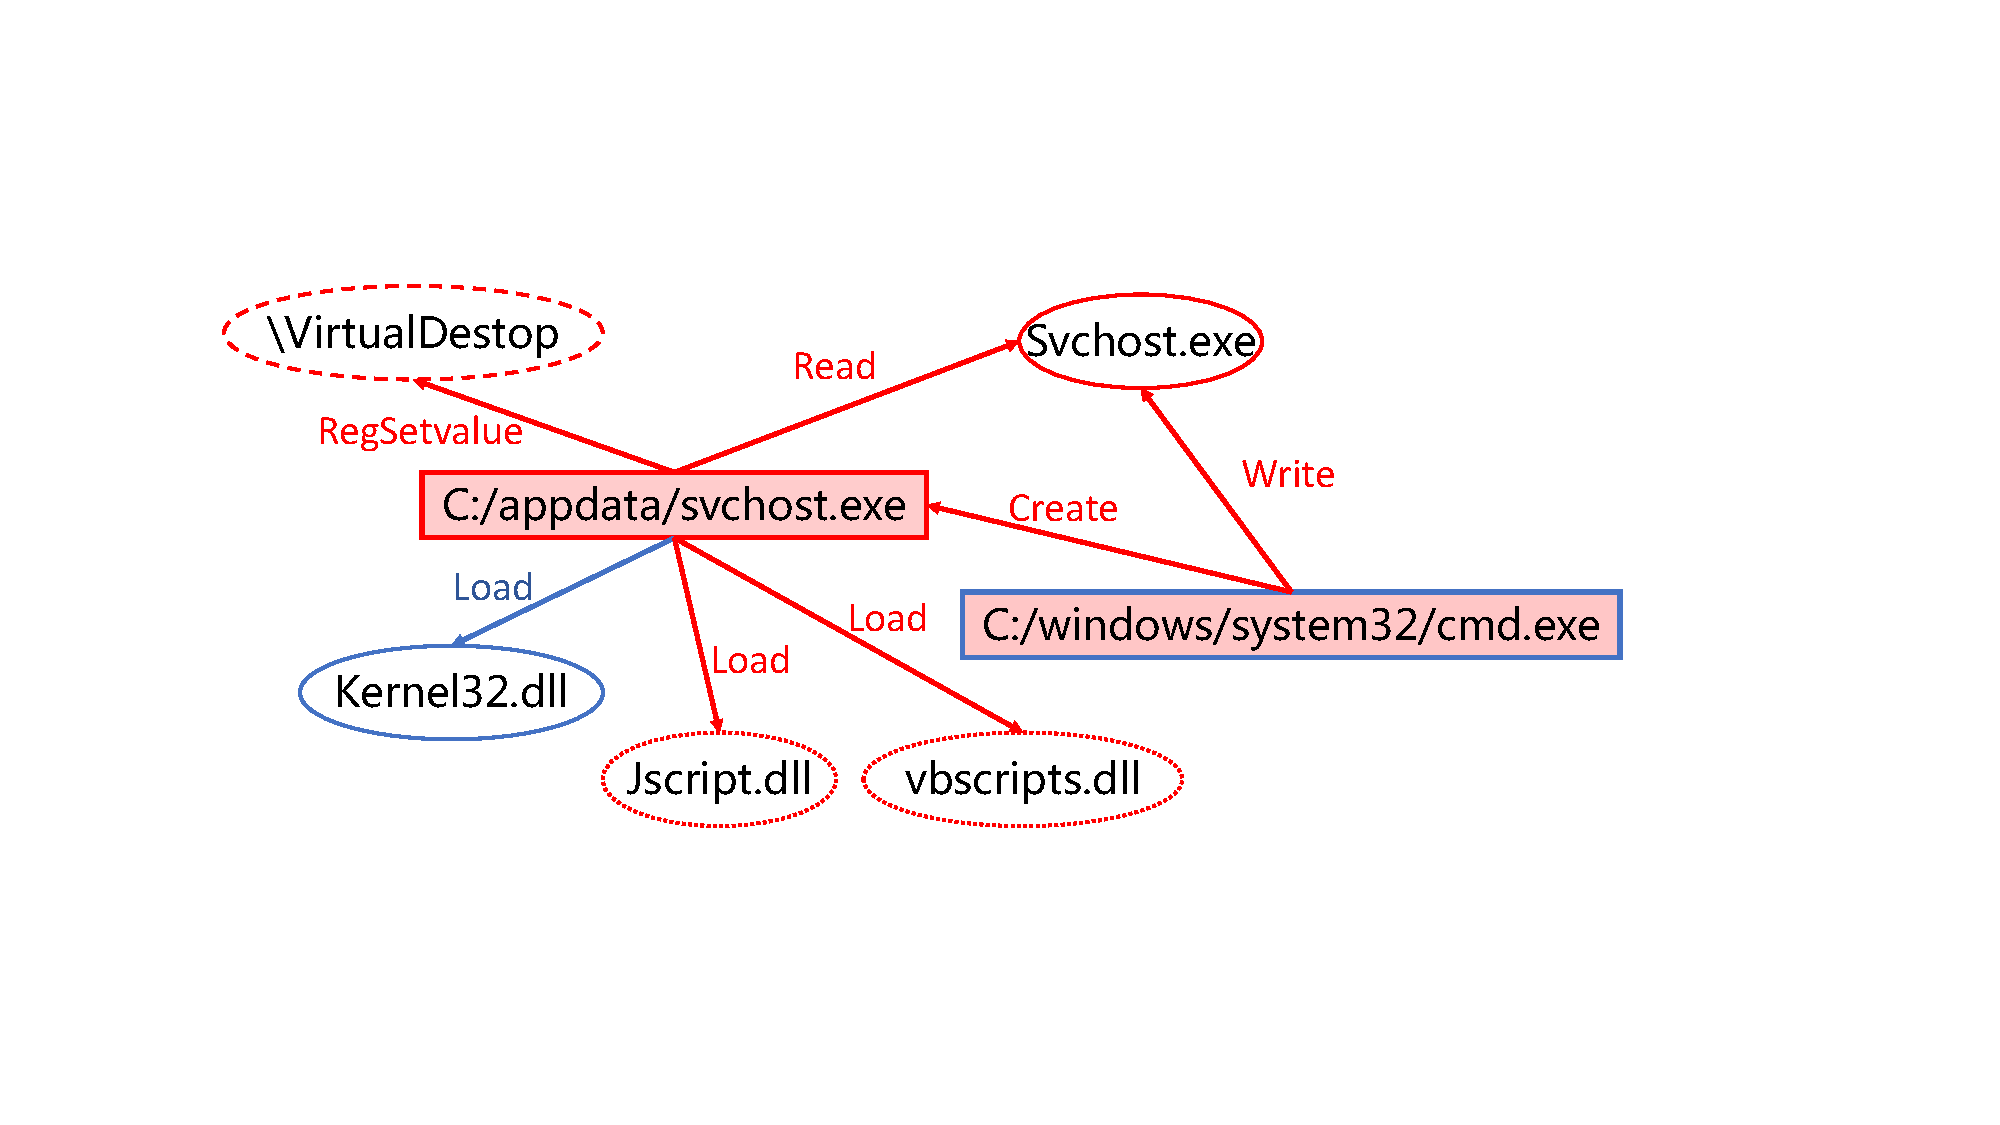
\includegraphics[width=\textwidth]{figs/Process Masquerade.pdf}
      \caption{Process Masquerade}
      \label{fig:process_mas}

  \end{subfigure}
  \hfill
  \begin{subfigure}{.5\textwidth}
      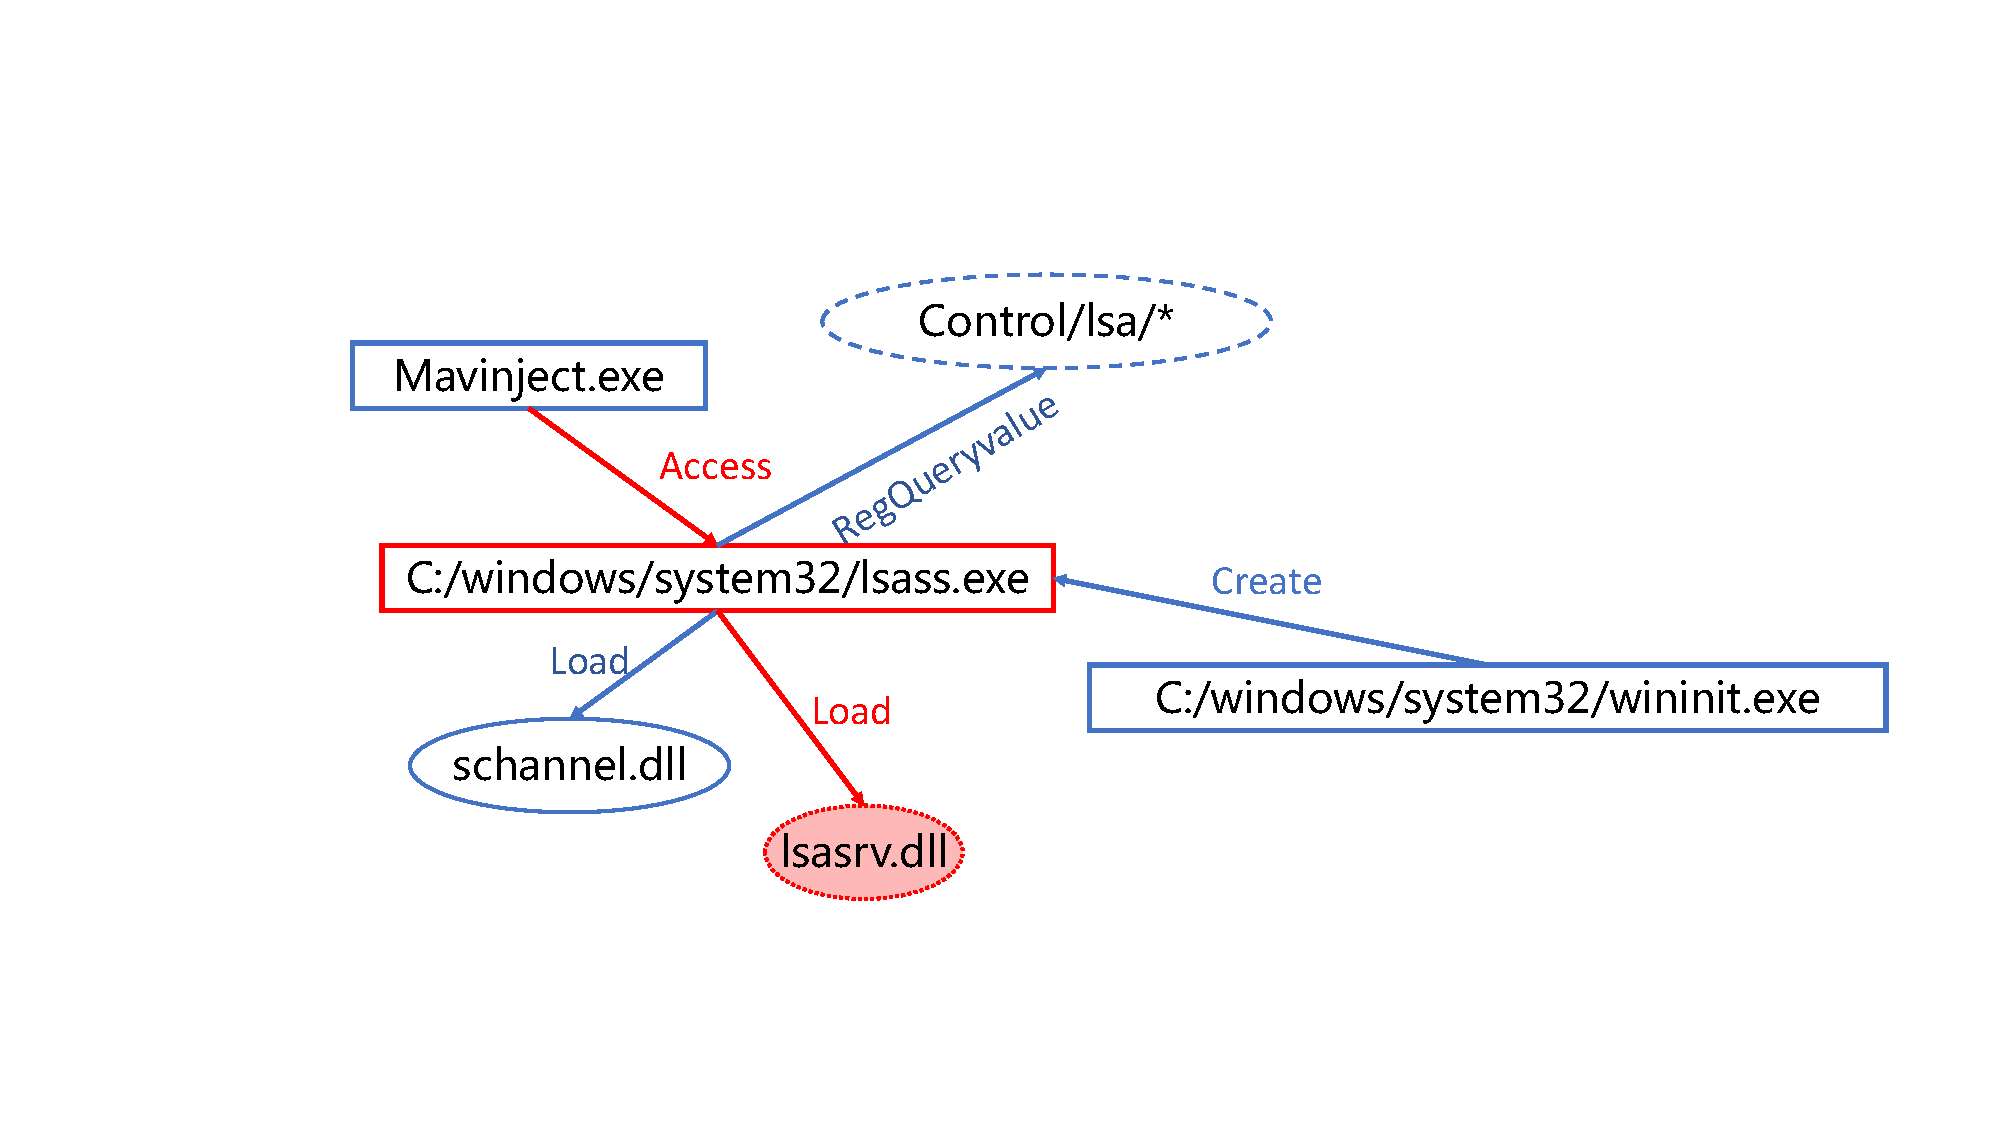
\includegraphics[width=\textwidth]{figs/process_injection.pdf}
      \caption{Process Injection}
      \label{fig:process_inj}

  \end{subfigure}

  \begin{subfigure}{.5\textwidth}
      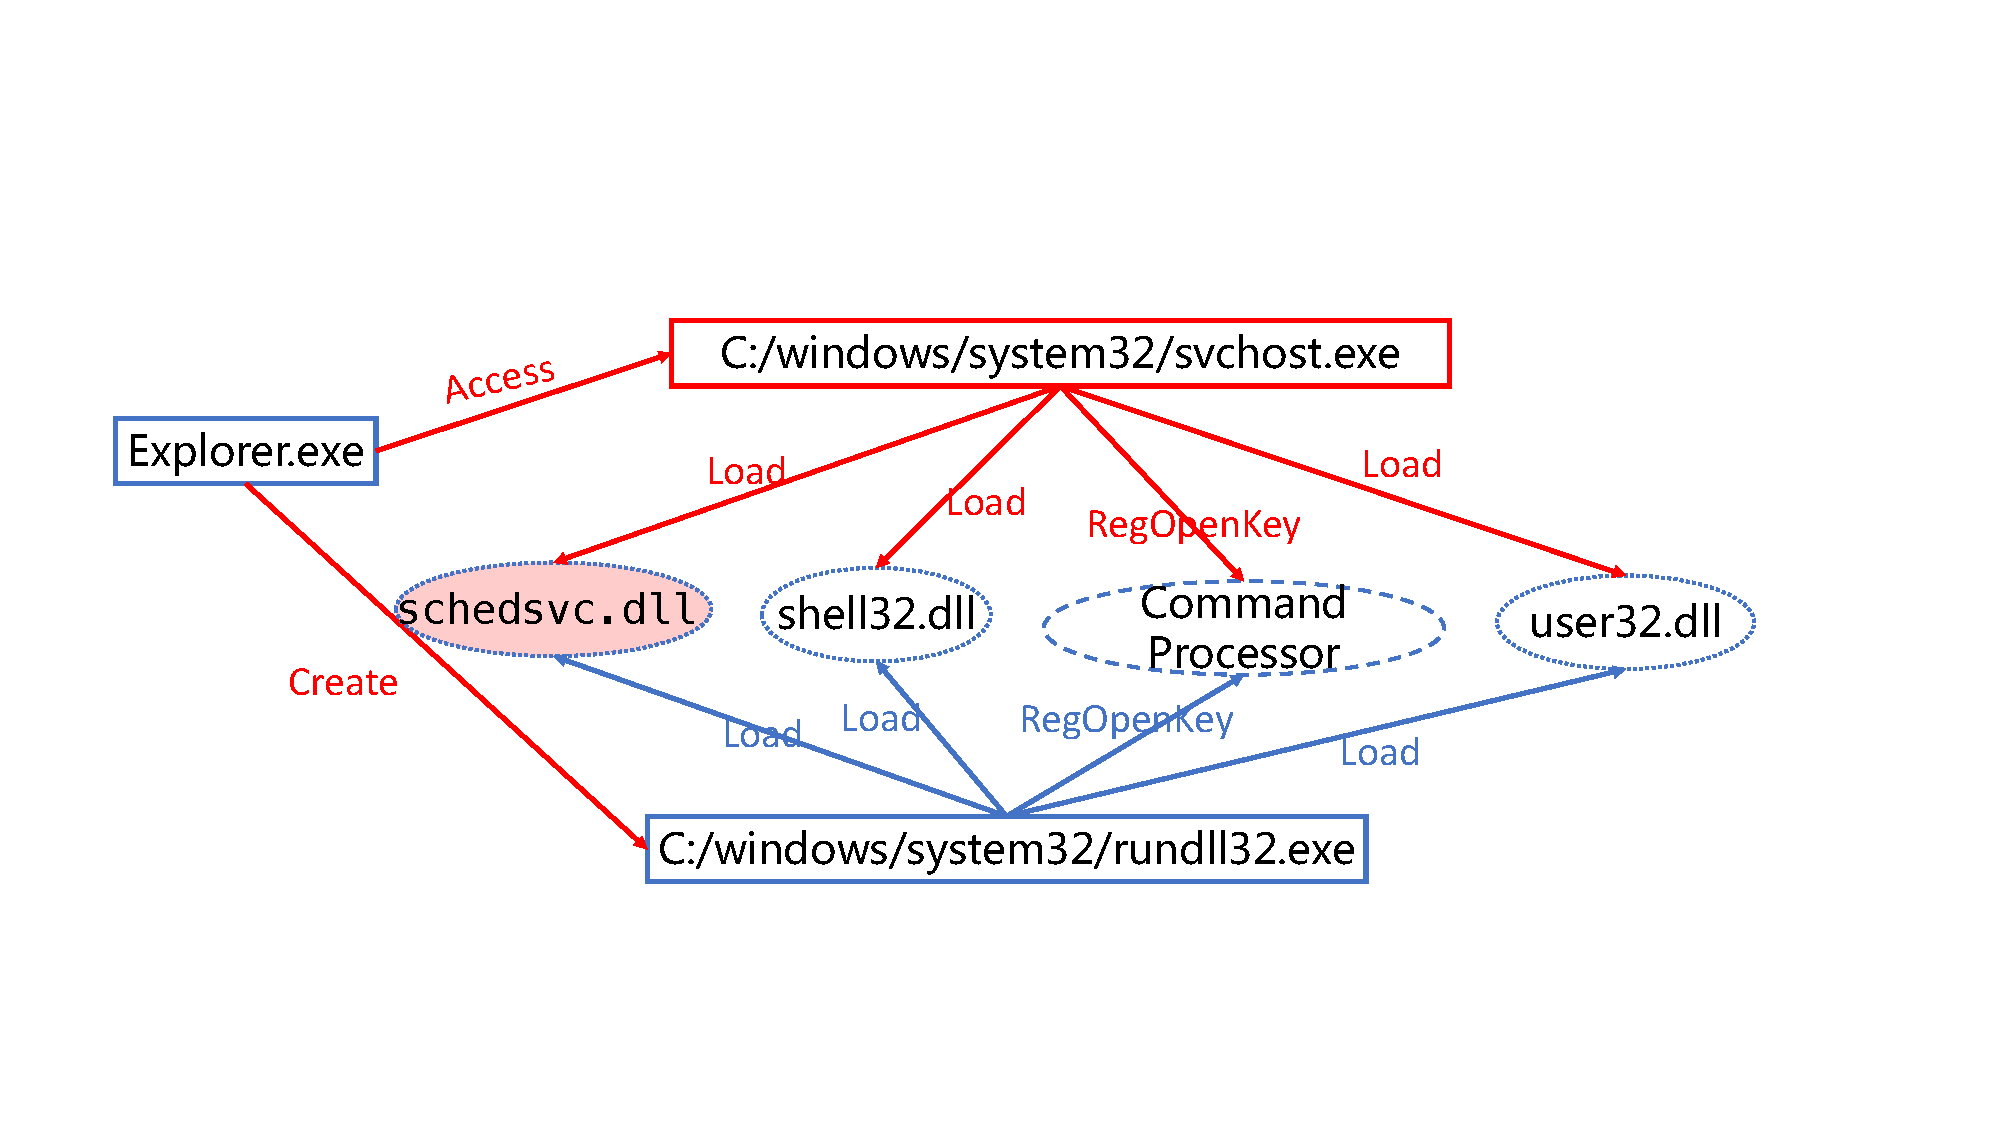
\includegraphics[width=\textwidth]{figs/Process Hollow.pdf}
      \caption{Process Hollow}
      \label{fig:hollow}

  \end{subfigure}
  \hfill
  \begin{subfigure}{.5\textwidth}
      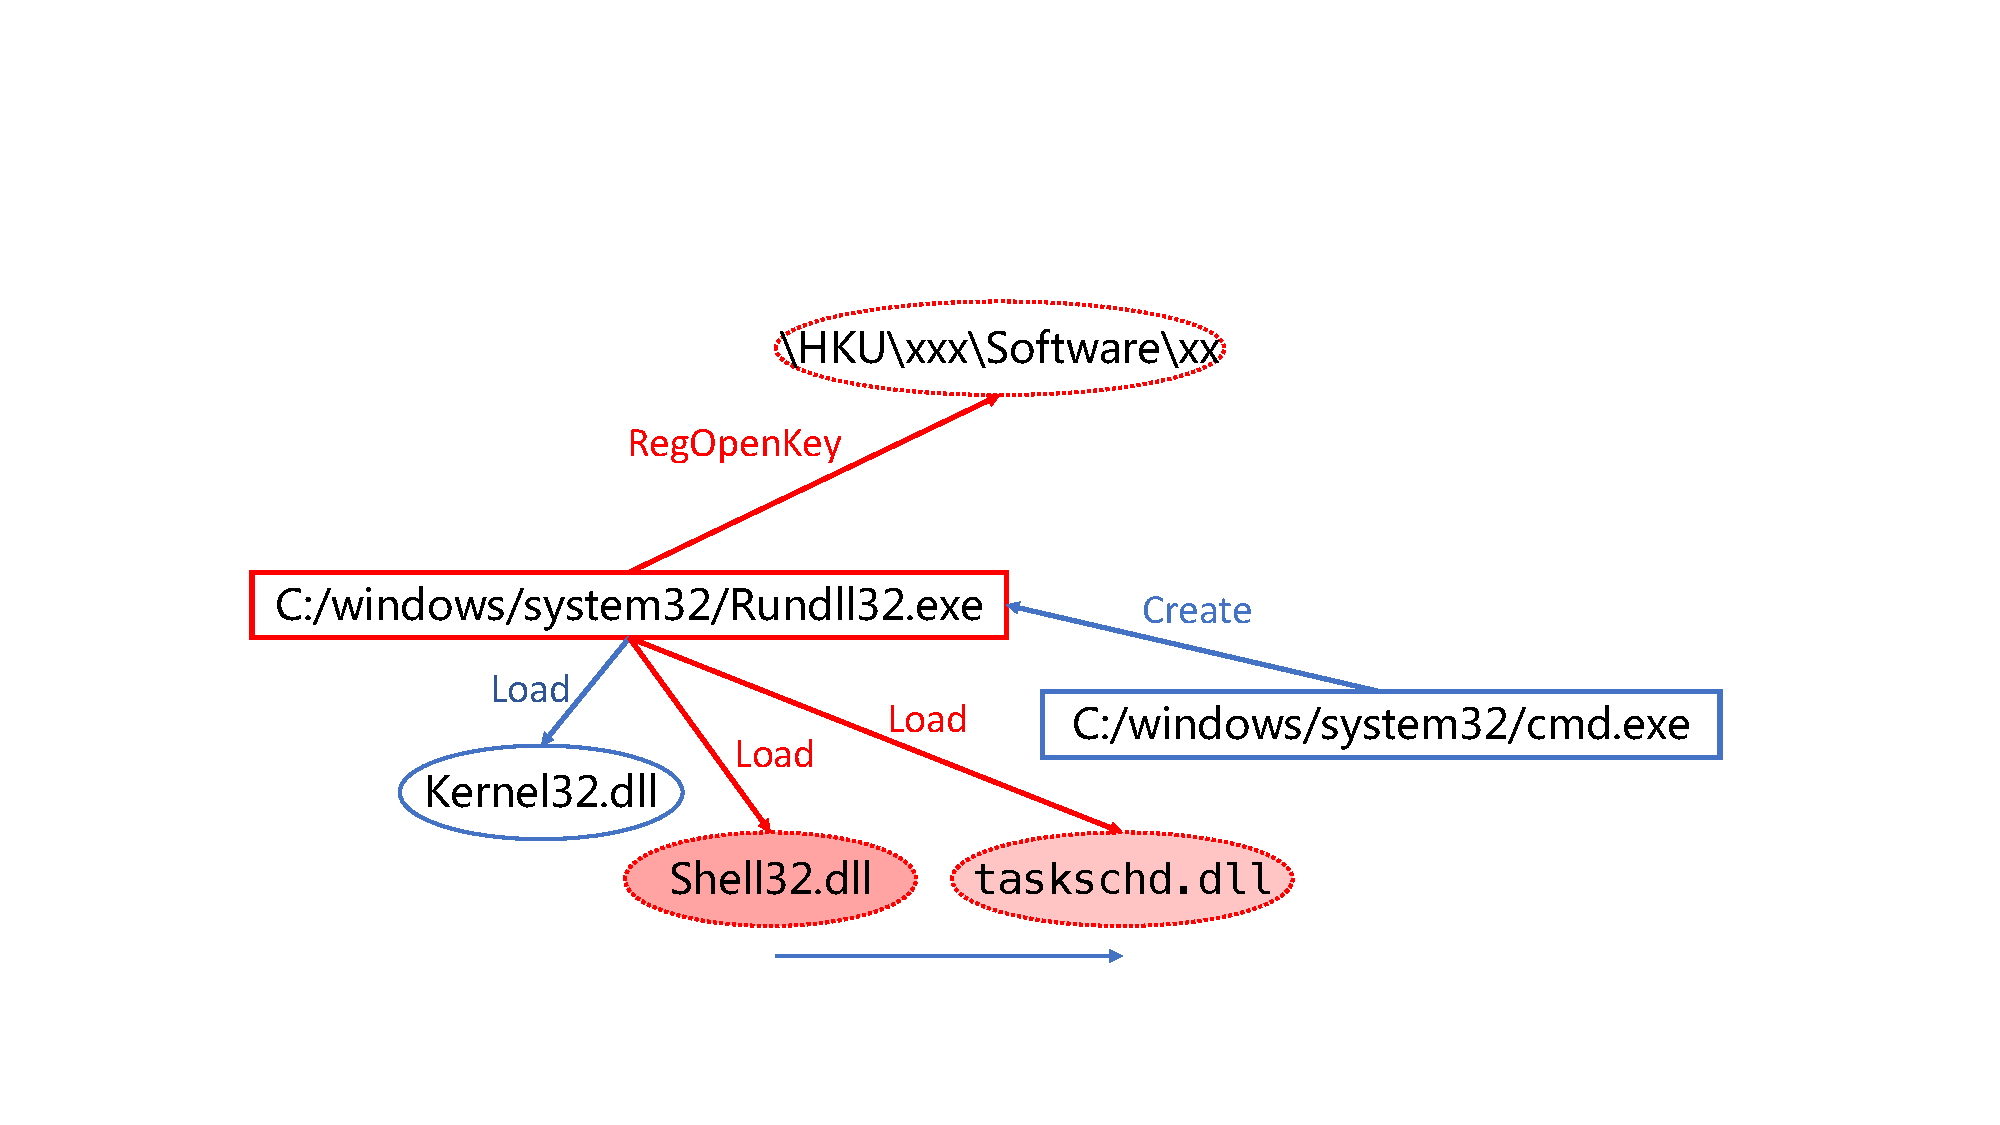
\includegraphics[width=\textwidth]{figs/Dll Side-Loading.pdf}
      \caption{Dll Side-Loading}
      \label{fig:side-load}
  \end{subfigure}

  \centering
 \caption{Each solid node in the graph represents detected signal, which has violated various constraints.}
\end{minipage}
\hfill
\begin{minipage}[b]{0.34\textwidth} 

  \begin{subfigure}{.99\textwidth}
      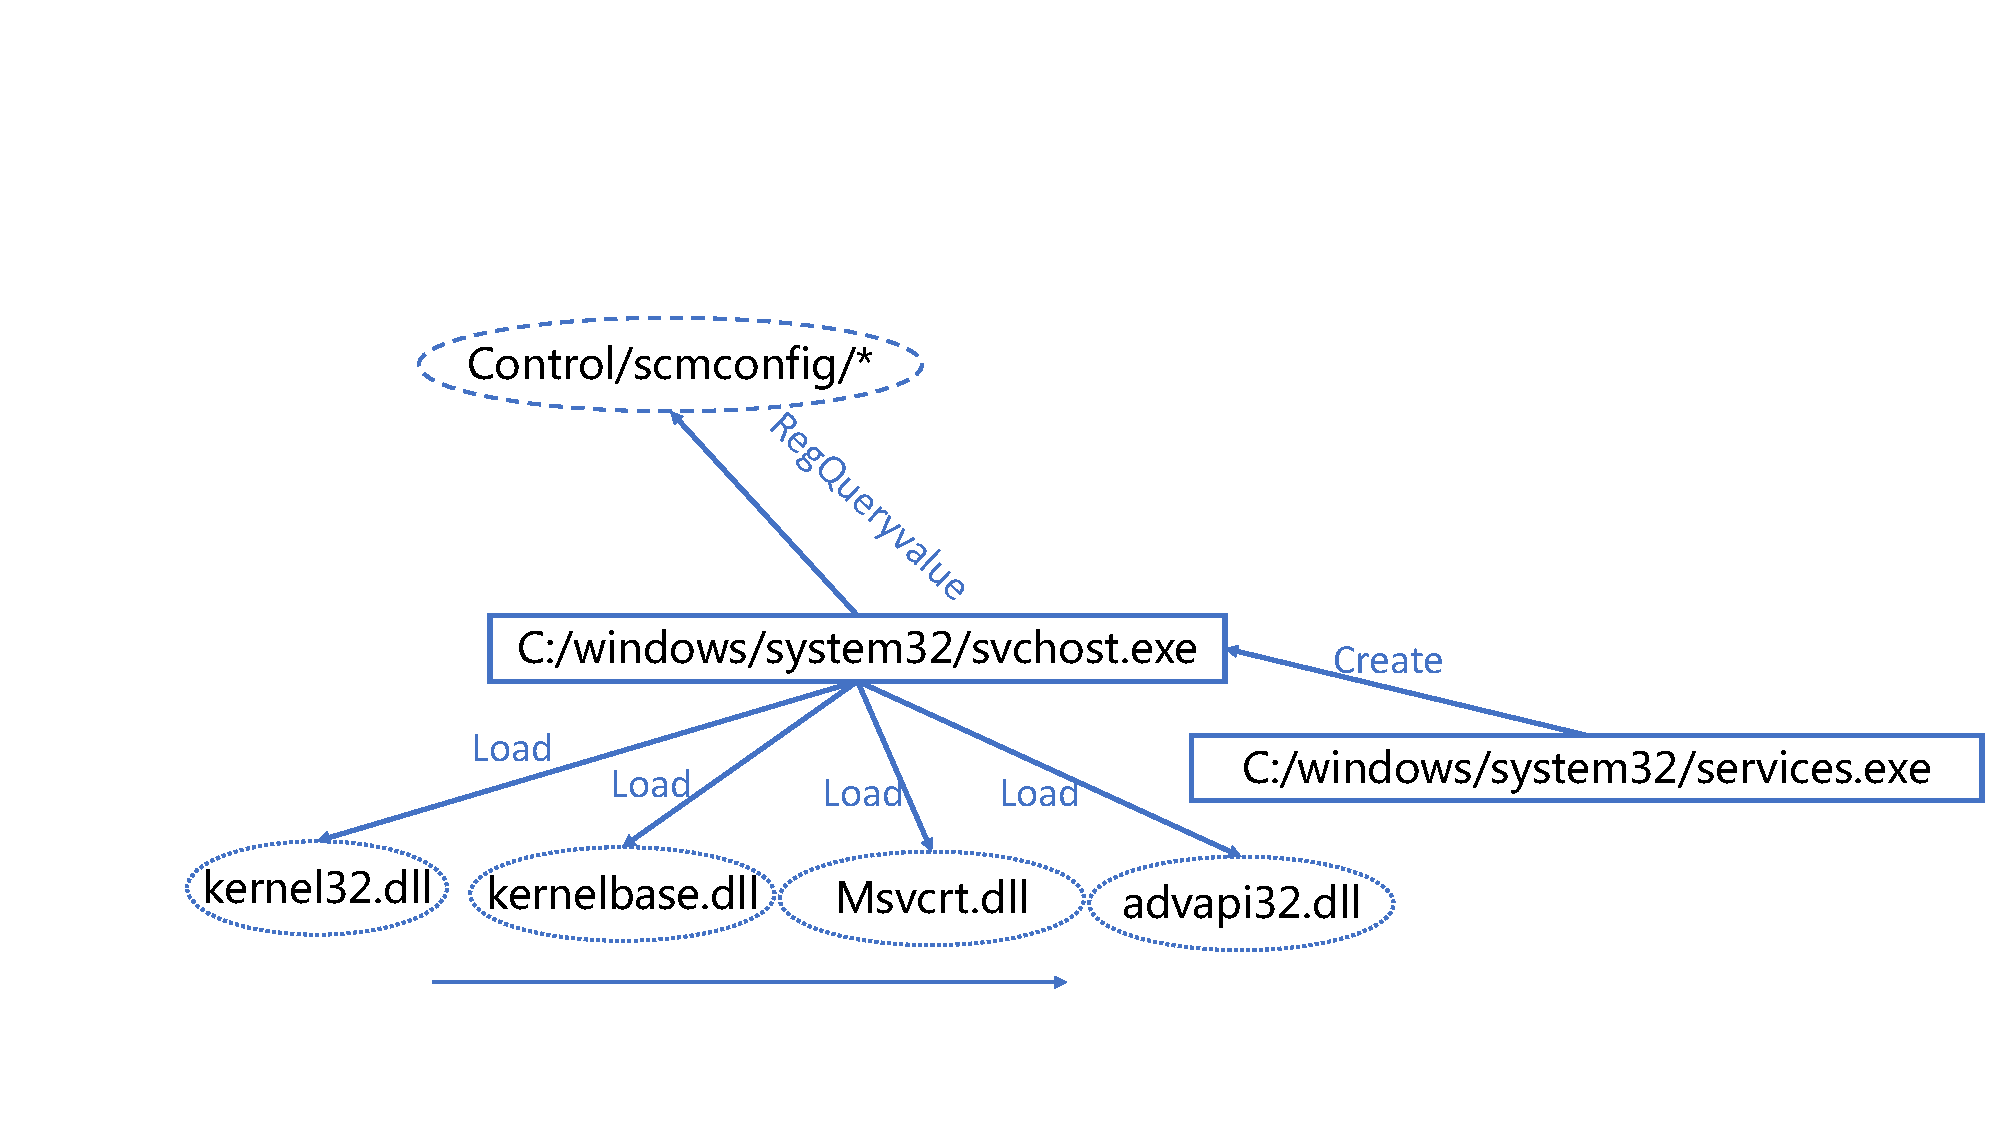
\includegraphics[width=\textwidth]{figs/svchost.pdf}
      \caption{Svchost Constraints}
      \label{fig:svc-cons}
  \end{subfigure}
  \hfill
  -\vspace{0.9cm}
  \begin{subfigure}{.99\textwidth}
      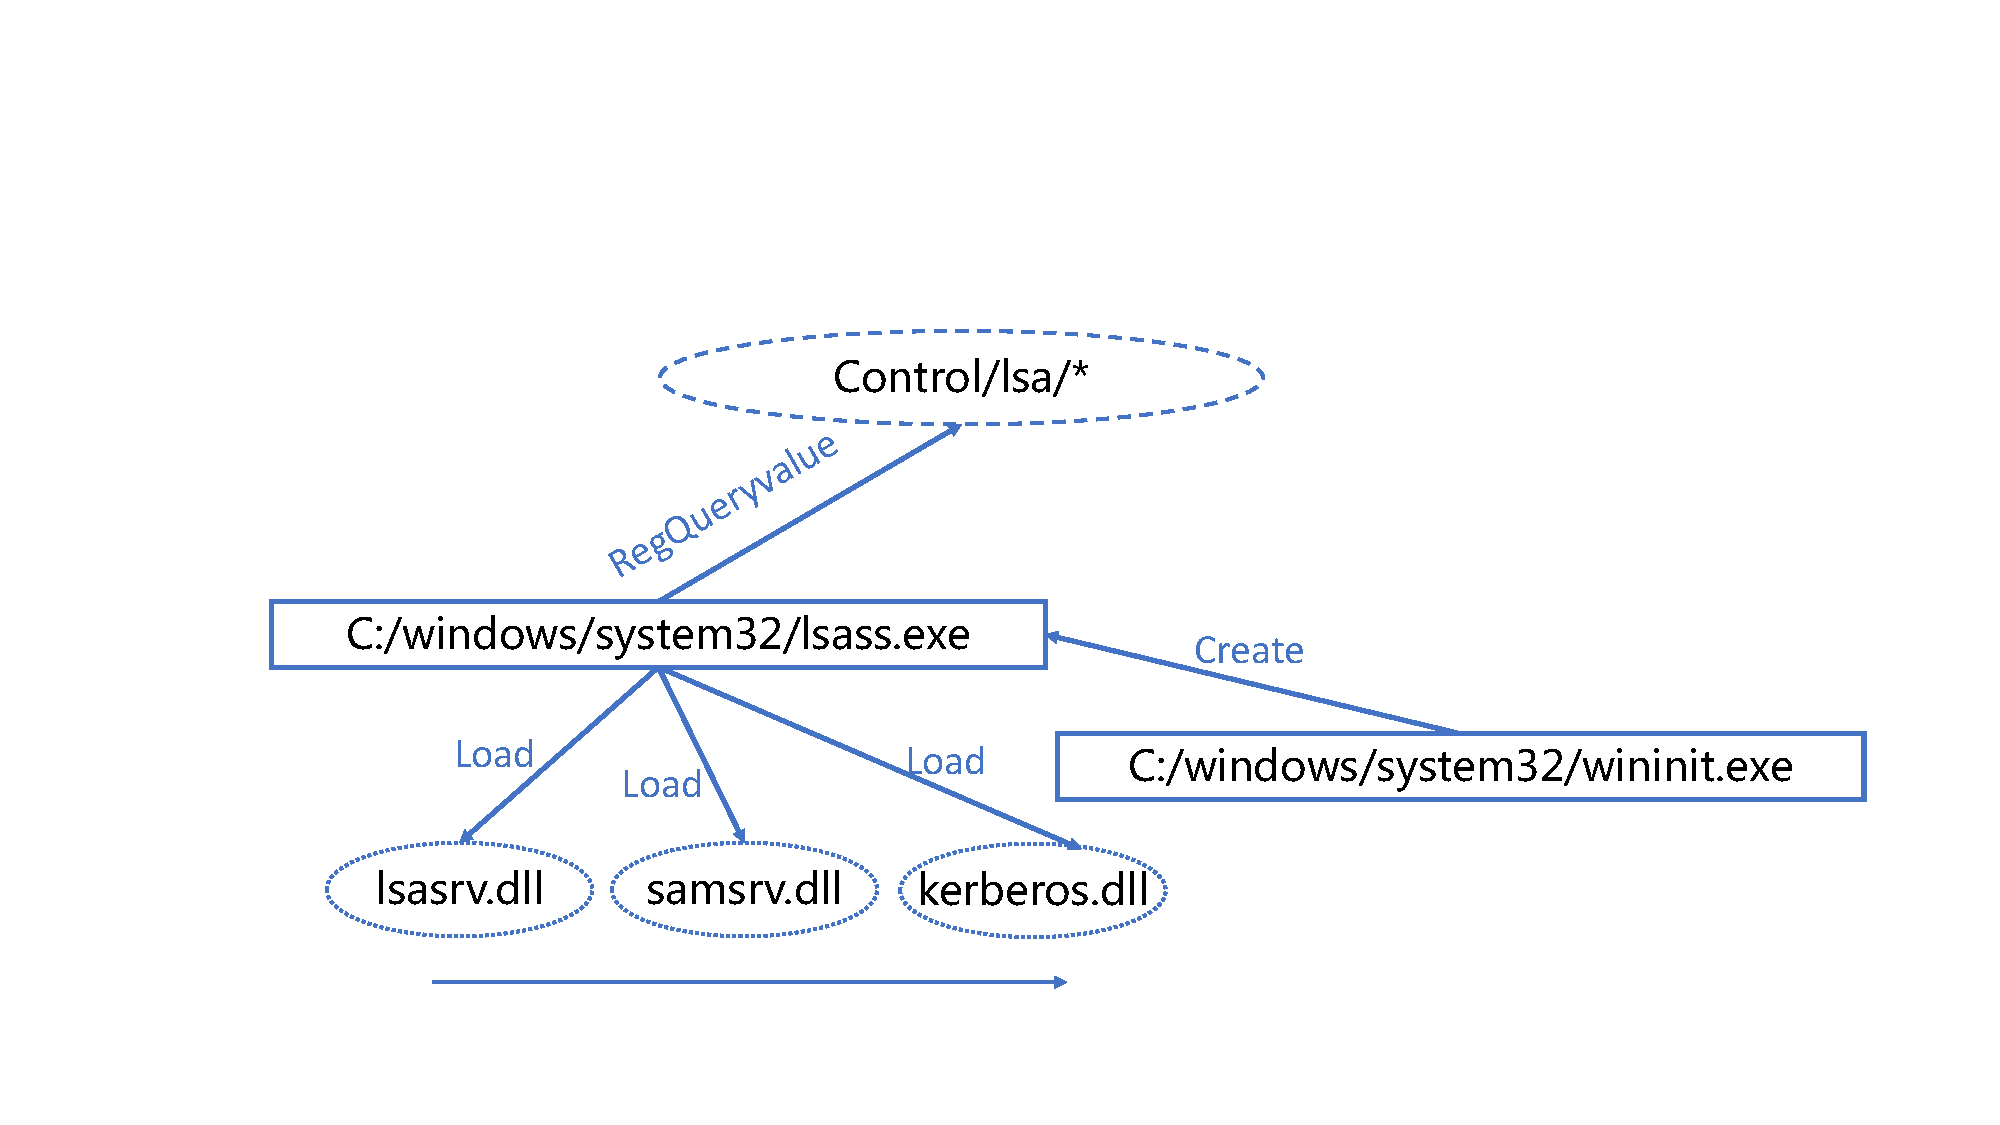
\includegraphics[width=\textwidth]{figs/lsass.pdf}
      \caption{Lsass Constraints}
      \label{fig:lsass-cons}
  \end{subfigure}
\caption{Constraints}
\label{fig-fdh}
\end{minipage}
\end{figure*}

\subsubsection{Evaluation on Attack for Various Processes}
We launched attacks on 100 system processes using 4 stealthy techniques, targeting 10 malicious functionalities. As illustrated in the Table~\ref{table:eva-attack}, it's evident that our method achieves a low false negative rate. However, some errors still persist, which we intend to delve into further.

\begin{table*}[h!]
    \centering
    \begin{tabularx}{\textwidth}{|X|X|X|X|X|X|X|X|X|X|X|}
        \hline
        & \textbf{BU} & \textbf{C} & \textbf{FM} & \textbf{FS} & \textbf{ST} & \textbf{PE} & \textbf{KM} & \textbf{FA} & \textbf{SE} & \textbf{E} \\
        \hline
\multicolumn{1}{|l|}{\textbf{PM}} & \multicolumn{1}{l|}{59/60}   & \multicolumn{1}{l|}{59/60}  & \multicolumn{1}{l|}{59/60}   & \multicolumn{1}{l|}{59/60}   & \multicolumn{1}{l|}{59/60}   & \multicolumn{1}{l|}{59/60}   & \multicolumn{1}{l|}{59/60}   & \multicolumn{1}{l|}{59/60}   & \multicolumn{1}{l|}{59/60}   & \multicolumn{1}{l|}{59/60}  \\ \hline
\multicolumn{1}{|l|}{\textbf{PH}} & \multicolumn{1}{l|}{59/60}   & \multicolumn{1}{l|}{57/60}  & \multicolumn{1}{l|}{57/60}   & \multicolumn{1}{l|}{58/60}   & \multicolumn{1}{l|}{58/60}   & \multicolumn{1}{l|}{59/60}   & \multicolumn{1}{l|}{57/60}   & \multicolumn{1}{l|}{57/60}   & \multicolumn{1}{l|}{59/60}   & \multicolumn{1}{l|}{60/60}  \\ \hline
\multicolumn{1}{|l|}{\textbf{PI}} & \multicolumn{1}{l|}{56/60}   & \multicolumn{1}{l|}{55/60}  & \multicolumn{1}{l|}{57/60}   & \multicolumn{1}{l|}{59/60}   & \multicolumn{1}{l|}{57/60}   & \multicolumn{1}{l|}{58/60}   & \multicolumn{1}{l|}{59/60}   & \multicolumn{1}{l|}{57/60}   & \multicolumn{1}{l|}{57/60}   & \multicolumn{1}{l|}{58/60}  \\ \hline
\textbf{DLL}                      & 59/60                        & 58/60                       & 57/60                        & 57/60                        & 59/60                        & 56/60                        & 57/60                        & 57/60                        & 58/60                        & 56/60                       \\ 
        \hline
    \end{tabularx}
    \caption{Detection of Process Count for Various Techniques and Malicious Activities.}
    \smallskip
    \small \textit{Abbreviations: BU - BypassUAC, C - Compress, FM - File Monitor, FS - File Scan, ST - Scheduled Task, PE - Privilege Escalation, KM - Keyboard Monitor, FA - Forced Authentication, SE - Service Execution, E - Exfiltration, PM - Process Masquerade, PH - Process Hollow, PI - Process Injection, DLL - DLL Side-Loading}
    \label{table:eva-attack}
\end{table*}
\smallskip
\noindent
{\bf Analysis of False Negatives.}
We discovered two primary reasons for these errors after thoroughly examining the incorrect cases:
\begin{itemize}
    \item \textbf{Some stealthy attack does not violate a constraint}: There are some stealthy attacks that do not violate any established constraints. For example, some rundll32.exe attack operates within its legitimate bounds. Live-off-ground attacks leverage the normal functionality of legitimate programs for malicious purposes.

    \item \textbf{Insufficient Knowledge for Certain Processes}:  The internal knowledge of the large language model is limited for some processes. Consider the process \textit{amdfendrsr.exe}(AMD Crash Defender Service), which is a core system process associated with the executable file \textit{amdfendrsr.exe}. The existing knowledge base lacks comprehensive details on this process. Consequently, the constructed profile results in weak constraints, which render the model incapable of detecting attacks that violate the \textit{amdfendrsr.exe} process constraints.
\end{itemize}
Given these findings, it's imperative to address these gaps to enhance the efficacy of our attack detection approach.


\subsubsection{Evaluation on Normal Workloads}
As previously mentioned, we sourced logs from different Windows versions from GitHub\cite{evtx-baseline2022}, specifically Windows 7, Windows 10, and Windows 11. These logs were collected from various users performing an array of routine operations. We utilized these logs to assess the false positive rate (i.e., false alarms) of our method in these scenarios.

In the Windows 7 scenario, our investigation encompassed 13 processes from our list, which manifested in 159 distinct entities due to multiple entities associated with a single process name. For Windows 10, we analyzed 47 processes (564 entities), and for Windows 11, we focused on 52 processes (1137 entities).

\begin{figure}[h]
    \centering
      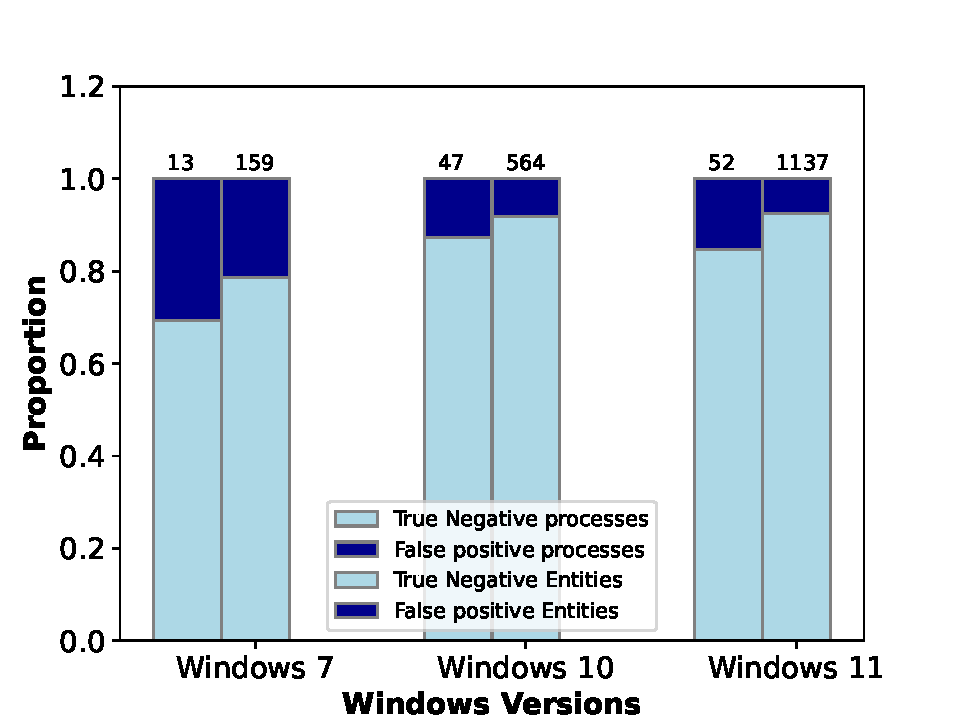
\includegraphics[width=0.49\textwidth]{figs/normal_chart.pdf}
    \caption{Evaluation on Normal Workloads.}
    \label{fig-eva-normal}
\end{figure}

\smallskip
\noindent {\bf Analysis of False Positives.}
After a detailed analysis of the various causes of false positives, we identified the following key issues:

\begin{itemize}
    \item \textbf{Uniformity in LLM's Results:} The LLM system tends to offer overly single results. For instance, the parent processes of \textit{C:/Windows/explorer.exe} can vary widely, including options like \textit{C:/Windows/explorer.exe} itself and \textit{C:/Windows/System32/svchost.exe}. However, LLM only provides feedback for \textit{userinit.exe}. This means that any normal process not having \textit{userinit.exe} as its parent process gets flagged incorrectly. This issue is also evident in processes like \textit{dllhost.exe} and \textit{conhost.exe} which can have multiple parent processes.
    \item \textbf{Overconfidence in LLM's Analysis:} For some events that might be absent in a few scenarios, the LLM tends to be overly confident. A case in point is the event \textit{(lsass.exe RegSetValue,hklm/system/currentcontrolset/control/lsa/*)}. While this event is expected to occur in the majority of scenarios, there are specific situations where it might not manifest. As a result, standard events get flagged erroneously. Another example includes a set of three events:\textit{(lsass.exe,Load Image,c:/windows/system32/lsasrv.dll->lsass.exe,Load Image,c:/windows/system32/samsrv.dll->lsass.exe,Load Image,c:/windows/system32/kerberos.dll)}. Typically, these events appear together. However, the event associated with kerberos.dll can sometimes be absent or loaded ahead of time. Consequently, having a stringent expectation for normal programs to execute in a specific order leads to false alarms.
    \item \textbf{Operating System Version Discrepancies:} Our process profile was built based on Windows 10 scenarios. As a result, while false positives are lower in a Windows 10 environment, they're notably higher for Windows 7. This is because Windows 10, being a newer version compared to Windows 7, has undergone changes in process behavior. For instance, in Windows 7, a single \textit{svchost.exe} might host multiple services. In contrast, in Windows 10, it can only host one. Consequently, profiles constructed for Windows 10 tend to have higher false positives when applied to Windows 7.
\end{itemize}


\subsubsection{Evaluation on Simulated APT scenarios}
We construct 10 simulated APT attack scenarios by combining single attack behavior and compare our method against four state-of-the-art techniques. By analyzing cases where current methods exhibit false positives, we aim to explain why these methods might produce false positives.

\begin{figure}[ht]
    \centering
      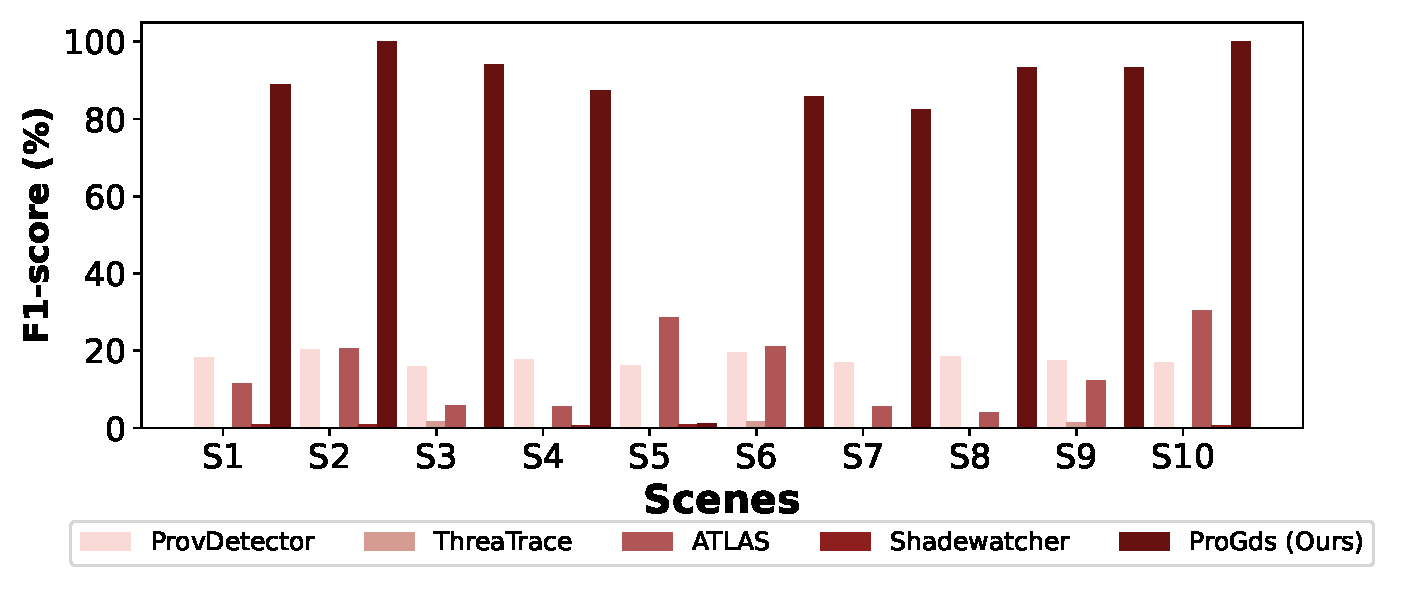
\includegraphics[width=0.49\textwidth]{figs/compare.pdf}
    \caption{Evaluation on Simulated APT scenarios.}
    \label{fig-eva-apt}
\end{figure}

\begin{itemize}
    \item \textbf{ThreaTrace}\cite{wang2022threatrace} An algorithm that constructs unique models for each type of node within a provenance graph aims to identify anomalies at the node level. Since this is a method based on anomalous nodes, we can compare the final false positive and false negative rates fairly.
    \item \textbf{ATLAS}\cite{alsaheel2021atlas} Uses graphs to derive attack and non-attack sequences, as well as sequence models to discern attack patterns. we compared the detection effect at the node level because our method is process-centered.
    \item \textbf{Shadewatcher} \cite{zengy2022shadewatcher} We have adapted the method originally designed for information flow for our comparative analysis. First, we use Shadewatcher's embedding method to get the node's vector, as soon as the embedding of the node is obtained, we use LOF anomaly detection to determine the detection rate of abnormal nodes.
    \item \textbf{ProvDetector.} A method analogous to ours is ProvDetector\cite{wang2020you}. It identifies malware by analyzing the provenance graph. In order to detect malware, it transforms paths within the graph into embedded representations and then uses the Local Outlier Factor technique. To evaluate the effectiveness of our method against ProvDetector, we analyzed results based on event investigation.
\end{itemize}


\begin{table}
    \centering
    \small 
    \begin{tabular}{|c|c|c|c|c|}
        \hline
        \multicolumn{1}{|c|}{Attack ID} & \multicolumn{2}{c|}{Process} & \multicolumn{2}{c|}{Entity} \\
        \cline{2-5}
        & \#Attack & \#Non-attack & \#Attack & \#Non-attack \\
        \hline
        S-1 & 8 & 738 & 41 & 2286 \\
        S-2 & 8 & 939 & 41 & 2669 \\
        S-3 & 9 & 1003 & 43 & 2704 \\
        S-4 & 7 & 713 & 18 & 2051 \\
        S-5 & 9 & 1134 & 45 & 3038 \\
        S-6 & 7 & 893 & 38 & 2277 \\
        S-7 & 8 & 718 & 21 & 2101 \\
        S-8 & 8 & 1092 & 42 & 2951 \\
        S-9 & 8 & 1090 & 42 & 2699 \\
        S-10 & 7 & 748 & 21 & 2157 \\
        Avg. & 8 & 907 & 35 & 2493 \\
        \hline
    \end{tabular}
    \caption{Process-based and entity-based investigation results.}
\end{table}

\begin{table}[ht]
\centering
\begin{tabular}{|l|c|c|c|}
\hline
\textbf{Method} & \textbf{P(Avg.)} & \textbf{R(Avg.)} & \textbf{F1(Avg.)} \\
\hline
ProvDetector & 17.82\% & 47.58\% & 47.85\% \\
ThreaTrace & 1.01\% & 35.84\% & 2.00\% \\
ATLAS & 9.63\% & 57.83\% & 14.68\% \\
Shadewatcher & 6.52\% & 0.20\% & 0.41\% \\
\tool & 94.44\% & 90.43\% & 91.33\% \\
\hline
\end{tabular}
\caption{Comparison of different methods.}
\label{tab:comparison}
\end{table}

% \begin{tabular}{|l|c|c|c|c|c|}
% \hline
% \textbf{Method} & \textbf{P(Avg.)} & \textbf{R(Avg.)} & \textbf{F1(Avg.)} & \textbf{Miss Rate} & \textbf{False Alarm Rate} \\
% \hline
% ProvDetector & 17.82\% & 47.58\% & 47.85\% & 52.42\% & 82.18\% \\
% ThreaTrace & 1.01\% & 35.84\% & 2.00\% & 64.16\% & 98.99\% \\
% ATLAS & 9.63\% & 57.83\% & 14.68\% & 42.17\% & 90.37\% \\
% Shadewatcher & 6.52\% & 0.20\% & 0.41\% & 99.80\% & 93.48\% \\
% \tool & 94.44\% & 90.43\% & 91.33\% & 9.57\% & 5.56\% \\
% \hline
% \end{tabular}

\textbf{Case Study.}
\begin{itemize}
    \item \textbf{Process Masquerade:} Process Masquerade imposes constraints on svchost.exe, as illustrated in Figure~\ref{fig:process_mas}. As a result of our method, we can observe that \textit{svchost.exe} normally executes in the path \textit{C:/windows/system32/svchost.exe}, with \textit{services.exe} as its parent process. Malicious \textit{svchost.exe} violates both execution path and parent process constraints in this example, resulting in its classification as malicious. Current methods \cite{wang2022threatrace} can detect this example if an overtly malicious activity is accompanied, such as port scanning, which results in noticeable changes in the graph structure. These methods fail to detect subtle malicious behaviors, such as executing services that do not alter the graph in a noticeable way.
    \item \textbf{Process Injection:} As illustrated in the Figure~\ref{fig:process_inj}, the attacker injects a malicious \textit{lsasrv.dll} into the \textit{lsass.exe} process. However, a normal \textit{lsass.exe} process follows a specific load chain where \textit{lsasrv.dll} is definitely followed by the loading of \textit{samsrv.dll}. The violation of this temporal constraint indicates malicious activity.
    \item \textbf{Process Hollow:} Shadewatcher is designed to embed itself into every node. In a process hollowing attack as shown in Figure~\ref{fig:hollow}, the depicted \textit{svchost.exe} is hollowed out and the memory functionalities of \textit{cmd.exe} are injected into it. As a result, \textit{svchost.exe} and \textit{cmd.exe} manifest similar functionalities. If we employ Shadewatcher's method of embedding, both \textit{cmd.exe} and \textit{svchost.exe} will have comparable embeddings. Since \textit{cmd.exe} exhibits normal behavior, it becomes indistinguishable whether the behavior of \textit{svchost.exe} is malicious or not. This inability to differentiate results in the failure to detect the attack.
    \item \textbf{Dll side-Loading:} Similar to process injection, DLL Side-Loading also violates the normal load chain, indicating an aberration from the standard operating procedure, and thereby suggesting malicious activity.
\end{itemize}



\subsection{Efficiency}
\label{sec-eff}
Regarding the efficiency concerns of our system, we aim to investigate the following questions:
\begin{itemize}
    \item How long does it take for our method to construct a profile for each process?
    \item Which step in the process profile creation is the most time-consuming?
\end{itemize}

To determine this, we have divided the process profile construction into five steps. We then individually measure the runtime and costs for each step, as illustrated in the Table~\ref{tab:process_metrics}.

In our study, we found that the process behavior tree construction is the most time-consuming and expensive part of the project. It takes 21 minutes and \$3.51 to build a profile for a single process.

\begin{table}[h!]
    \centering
    \begin{tabular}{|l|c|c|}
        \hline
        & Running Time & Cost \\
        \hline
        Behavior Tree Construction & 501(s) & 1.23\$ \\
        \hline
        Command Generate & 156(s) & 0.85\$ \\
        \hline
        Command Execution & 200(s) & 0\$ \\
        \hline
        Constraint Extraction & 201(s) & 0.51\$ \\
        \hline
        Validation & 321(s) & 0.92\$ \\
        \hline
        Total & 1379(s) & 3.51\$ \\
        \hline
    \end{tabular}
    \caption{Running Time and Cost for various processes}
    \label{tab:process_metrics}
\end{table}

\subsection{Ablation Study}
\label{sec-ab-study}
A ablation study was conducted integrating data from 10 different attack scenarios with three normal scenarios, namely Windows 7, Windows 10, and Windows 11. In total, the attack scenarios included 80 attack processes, while the normal scenarios comprised 1960 regular processes.

The ablation study aims at assessing the effectiveness of the divergent and validation methods that are integral to \tool's performance. Our goal is to understand the contributions of two critical modules: the Process Tree Construction Module and the Validation Module. 
This experiment modified the approach by either removing one or both of these steps. As a result, three control groups were created:
\begin{itemize}
\item \textit{\tool-NO-Tree-Construction}: In this version, the Process Tree Construction Module is deactivated. This means all data is input directly into the system without any hierarchical structuring.
\item \textit{\tool-NO-Validation}: What would be the accuracy of our method if we were to skip the validation step?
\item \textit{\tool-NO-All}: This indicates that the process tree Construction and validation steps have both been removed.
\end{itemize}

\begin{figure}[h]
    \centering
    \begin{subfigure}[b]{0.23\textwidth}
        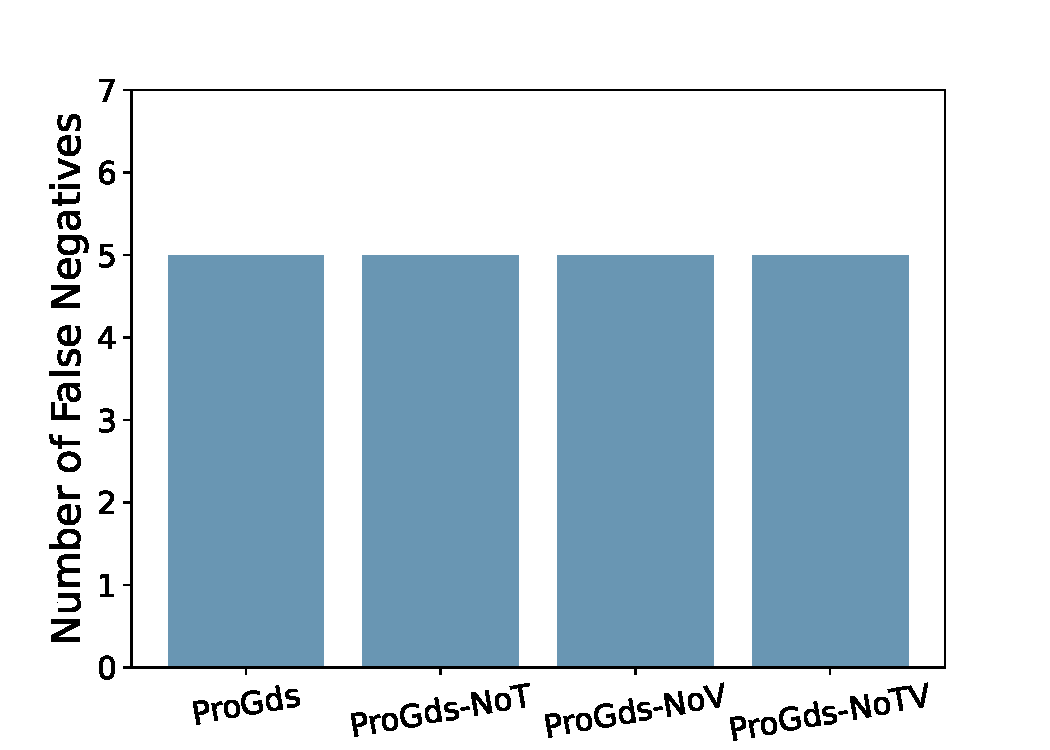
\includegraphics[width=\textwidth]{figs/FN.pdf}
        \caption{False Negative for In Attack Scenario}
        \label{fig:missed_attacks}
    \end{subfigure}
    \hfill
    \begin{subfigure}[b]{0.23\textwidth}
        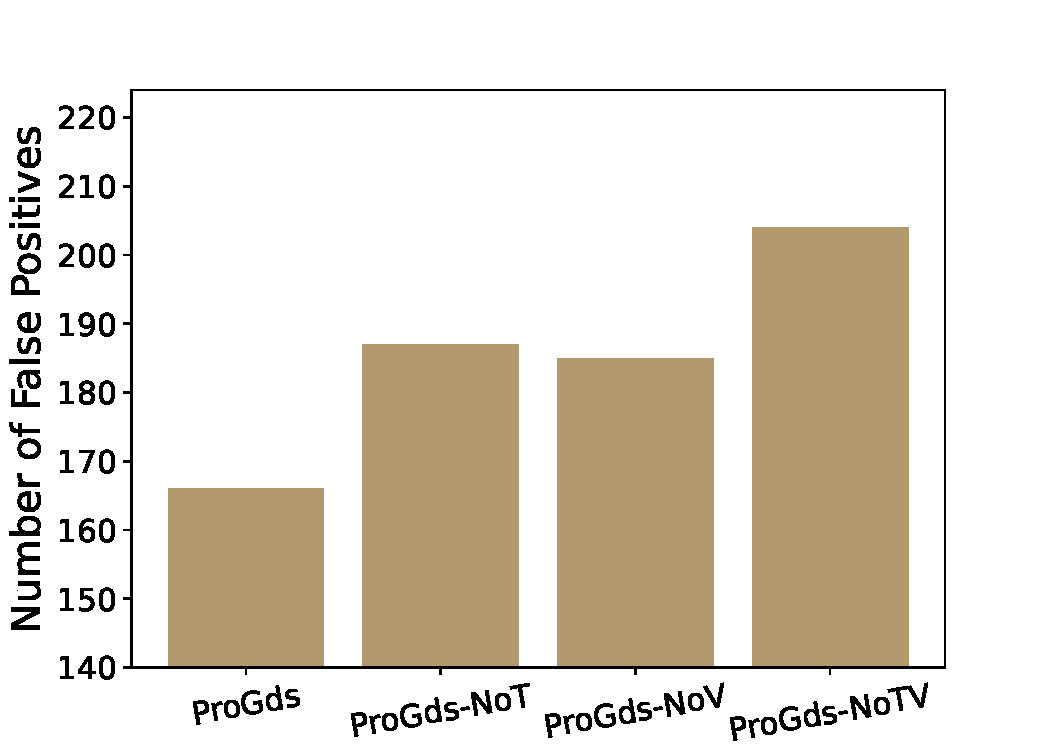
\includegraphics[width=\textwidth]{figs/FP.pdf}
        \caption{False Positives for Normal Scenario}
        \label{fig:false_positives}
    \end{subfigure}
    \caption{Comparison of different methods in terms of False Negative and false positives}
    \label{fig:comparison}
\end{figure}
We found no significant difference in attack scenarios between our method and the control method. Our approach, however, achieved the lowest false positive rate for normal scenarios.

In the following, examples are used to illustrate the role of adding behavior trees and validation links in reducing false positives.
Without the construction of the behavior tree, we obtain many constraints that are too broad.
For example, the behaviors that we mind and that \textit{svchost.exe} must obey when hosting certain services, like \textit{PhoneSvc} and \textit{NgcSvc}, must have behavior \textit{svchost.exe,CreateFile,*/localservice/appdata*}. However, for other services like the \textit{DHCP service}, this behavior isn't necessarily required.
These are not behaviors that all processes must adhere to, resulting in a high false positive rate when tested normally. 

We aim to demonstrate the effectiveness of our cross-session validation approach. To this end, we've introduced a novel validation method: employing three agents to engage in a debate to validate behaviors. From our experiments, it's evident that for actions that are undeniably factual, the three agents can reach a consensus after multiple rounds of debate. For instance, \textit{lsass.exe} will unquestionably load \textit{c:/windows/system32/lsasrv.dll}. On the other hand, for behaviors that aren't necessarily factual, the agents diverge in their opinions after several debate rounds and pinpoint the underlying reasons. For example, the behavior of \textit{sass.exe} with \textit{RegSetValue, hklm/system/currentcontrolset/control/lsa/} is not mandatory.



\subsection{Explanation Validation}
\label{sec-explanation-val}

Detection and interpretation are seamlessly integrated into our approach. The following sections explain how our method exposes attack behaviors and facilitates rapid verification and response to threats by security analysts.
To confirm the accuracy of the constraints we extracted, we searched Google, blogs, books, etc. In some public reports, we found consistency between their findings and our constraints.

There is some crucial document online\cite{nasbench}, including a technical document that outlines the execution paths and parent-child processes of 15 essential system processes. For instance, in the case of lsass.exe, the document indicates that its parent process is wininit.exe, it does not have a fixed child process, and its execution path is \textit{\%Systemroot\%/system32/lsass.exe}. It aligns with the knowledge we have gained through LLMs.
There is also document\cite{windows10dll} about static call relationship between Windows DLLs. \textit{Lsass.exe} will undoubtedly load \textit{lsasrv.dll}, and \textit{lsasrv.dll} and \textit{samsrv.dll} have a static link relationship. This knowledge also remains consistent with what we have learned through LLMs.
Through our analysis, it seems possible that the LLM might have learned from these documents. We have not found any specific references to support some illusions generated by LLMs.

% https://nasbench.medium.com/windows-system-processes-an-overview-for-blue-teams-42fa7a617920

% https://windows10dll.nirsoft.net/lsasrv_dll.html

\subsection{Real-world Validation}
\label{sec-real-world}

We collected some publicly available malicious software related to APTs, as shown in the Figure~\ref{tab:real_world}.
In some cases, such as for APT29, we were able to retrieve the original collected data directly, while in others we could only retrieve the dynamic execution logs from the VirusTotal sandbox. Using this real-world data, we wanted to verify the effectiveness of our method. As a result of the results, we can detect most types of stealth attacks using our method, including these four types of stealth attacks.

\begin{itemize}
    \item APT29 \cite{mitre_g0016}: We have analyzed malicious payloads associated with APT29, specifically focusing on \textit{python.exe}. According to the profile we constructed for a typical Python application, \textit{python.exe} would certainly load \textit{pythonxx.dll} and \textit{vcruntime140.dll}. However, in the dataset related to the malicious \textit{python.exe} used by APT29, we didn't find evidence of these two DLLs being loaded. This suggests that the \textit{python.exe} under scrutiny is likely not a standard or legitimate version.

    \item DCSrv\cite{checkpoint2021}: Moving on to the malware named DCSrv, we located this malicious software in the VirusTotal sandbox. We observed that it masquerades as \textit{svvhost.exe} with an execution path of \textit{C:/Users/user/Desktop/svvhost.exe}. \textit{Svchost.exe} has been obfuscated through string obfuscation, and its execution path is different from the typical \textit{svchost.exe} path.

    \item Sykipot\cite{att2023}: It appears that the malicious program Sykipot launches process injection attacks against \textit{firefox.exe}. The injected malicious dll is named \textit{wship4.dll}. There is no legitimate DLL by this name, but we did find \textit{wship6.dll}, which is related to IPv6 network operations. In order for \textit{wship6.dll} to interact correctly, \textit{WS2\_32.dll} must also be loaded. Furthermore, there was no indication that \textit{WS2\_32.dll} was loaded, indicating malicious activity.
\end{itemize}










\section{Discussion}

\noindent
{\bf Some attacks do not violate process constraints.}
There are some attacks that do not violate process constraints. For example, attackers can launch sophisticated attacks by using common tools such as \textit{rundll32.exe} and \textit{powershell.exe} in a manner that does not violate process constraints. However, LLMs still hold the potential to solve this problem. From a blacklist perspective, LLMs can explore more logical vulnerabilities. From a whitelist perspective, LLMs can establish behavioral constraints at the logical behavior level.

\noindent
{\bf Issues with Commands Generated by LLMs.}
Some commands cannot be executed in the system, and some are very difficult to run because they involve system processes. Also, it is challenging to determine whether some commands have been executed successfully.

\noindent
{\bf Incomplete Knowledge in LLMs.}
LLMs lack comprehensive knowledge. A lack of process information in LLMs can lead to detection failures. Using external security information to supplement missing data could be one solution.

\noindent
{\bf Hallucination Problems in LLMs.}
Although the accuracy of knowledge can be improved by using real logs and cross-session for validation, LLMs are difficult to completely eliminate illusions.


\section{Conclusion}


% %-------------------------------------------------------------------------------
% \section*{Acknowledgments}
% %-------------------------------------------------------------------------------

% The USENIX latex style is old and very tired, which is why
% there's no \textbackslash{}acks command for you to use when
% acknowledging. Sorry.

% %-------------------------------------------------------------------------------
% \section*{Availability}
% %-------------------------------------------------------------------------------

% USENIX program committees give extra points to submissions that are
% backed by artifacts that are publicly available. If you made your code
% or data available, it's worth mentioning this fact in a dedicated
% section.

% %-------------------------------------------------------------------------------
\bibliographystyle{plain}
%\bibliography{\jobname}
\bibliography{main}

\appendix
\section{Appendix}

\subsection{Prompt}

\subsubsection{Behavior Tree Construction Prompt}
\begin{tabularx}{\textwidth}{|c|X|}
\hline
\multicolumn{2}{|c|}{\textbf{Input:} \{process\_name\}} \\
\hline
\textbf{Goal} & You can receive a number of commands, each with a different function, which are used to help build the \{process\_name\} behavior tree. \\
\hline
\textbf{Role} & You are a security expert and you are familiar with the legal behavior of important windows processes. \\
\hline
\multirow{6}{*}{\textbf{Behavior Tree}} & The format of this knowledge tree is as follows: \\
& 1. basic profile \\
& 1.1. execution path \\
& 1.2. parent and child processes \\
& 1.3. permissions \\
& \dots \\
\hline
\multirow{5}{*}{\textbf{Commands}} & 1. Automatic Behavior Generator: Continuously ask important questions and extend behaviors based on the current behavior tree. \\
& 2. Manual Behavior Generator: I'll manually enter some questions and you get the appropriate answers based on those questions. \\
& 3. Update Behavior Tree: you update the knowledge tree with the information from the current session. \\
& 4. Important logs corresponding to specific behaviors: For some behaviors that can be executed in the system, execute them in the system to get log information. \\
& 5. Finish: use this to signal that you have finished all your objectives, args: "response": "final response to let people know you have finished your objectives". \\
\hline
\textbf{Note} & Integration of new and old knowledge when they overlap. \\
\hline
\textbf{History} & \dots \\
\hline
\end{tabularx}

\subsubsection{Commands Prompt}

\subsubsection{Prompt for explanation}



%%%%%%%%%%%%%%%%%%%%%%%%%%%%%%%%%%%%%%%%%%%%%%%%%%%%%%%%%%%%%%%%%%%%%%%%%%%%%%%%
\end{document}
%%%%%%%%%%%%%%%%%%%%%%%%%%%%%%%%%%%%%%%%%%%%%%%%%%%%%%%%%%%%%%%%%%%%%%%%%%%%%%%%

%%  LocalWords:  endnotes includegraphics fread ptr nobj noindent
%%  LocalWords:  pdflatex acks
